%!TEX root = ../report.tex

\begin{document}
    \chapter{Experimental Evaluation}\label{chap_exp_eval}
\section{Metrics}
\subsection{Root Mean Squared Error(RMSE)}
Root Mean Squared Error (RMSE), measures the spread of distances between model predictions and their corresponding ground truth values. Alternatively, it can be explained as the standard deviation of prediction errors. RMSE is a well-known accuracy metric in regression problems. The metric is non-negative in nature with lower values indicating better model fit.
\begin{equation}
	\mathbf{RMSE} = \sqrt{\frac{\sum_{i=1}^{N}(\hat{y}_i-y_i)^2}{N}}
\end{equation}
Here $\hat{y}$,$y$ and $N$ represent ground truth labels, predictions and number of data points respectively.
\subsection{Explained Variance(EVA)}
The Explained Variance (EVA) is a measure of a regressor's ability to capture variance(variation) of given data. The metric can be computed with the following expression:
\begin{equation}
	\mathbf{EVA} = 1-\frac{Variance(\hat{y}-y)}{Variance(\hat{y})}
\end{equation}
Here $\hat{y}$,$y$ represent ground-truth labels and predictions respectively. The numerator term denotes variance of residuals whereas the denominator denotes the underlying variance in ground-truth labels. For an ideal regressor, the value of EVA equals 1.
\subsection{Negative-Log-Likelihood(NLL)}
In this research work,the Negative-Log-Likelihood(NLL) metric is used compare performance of uncertainty estimation methods. NLL for a given pair of prediction and uncertainty can be computed as follows
\begin{itemize}
	\item A distribution (often Gaussian) is created with the model prediction as its mean and uncertainty as its variance.
	\item The conditional probability of observing the ground-truth label(corresponding to the input) in the created distribution is determined. This is nothing but the likelihood value of ground-truth in the created distribution.
	\item  In order to handle and effectively represent very low values of likelihood, negative of natural logarithm is applied  to the value. After application of negative logarithm, the total likelihood can be computed by summing all individual values.
\end{itemize}
\begin{equation}
	\mathbf{NLL} = -\sum_{i=1}^{N}\ln P(\hat{y}_i|\mathcal{N}(y_i,\sigma^2)) 
\end{equation}
Here $\hat{y}$,$y$,$\sigma^2$ and $N$ represent ground truth labels, predictions, predictive uncertainty and number of data points respectively.
Lower the value of NLL better the performance of an uncertainty estimation method associated with it. However, the value of NLL highly depends on the number and choice of test points used for evaluation. Therefore, the metric can be used to compare performance of uncertainty estimation methods only when the same data set is used for their evaluation.
\subsubsection{Limitations of NLL}
\begin{figure}[H]
\centering
\begin{subfigure}[b]{0.3\textwidth}
	\centering
	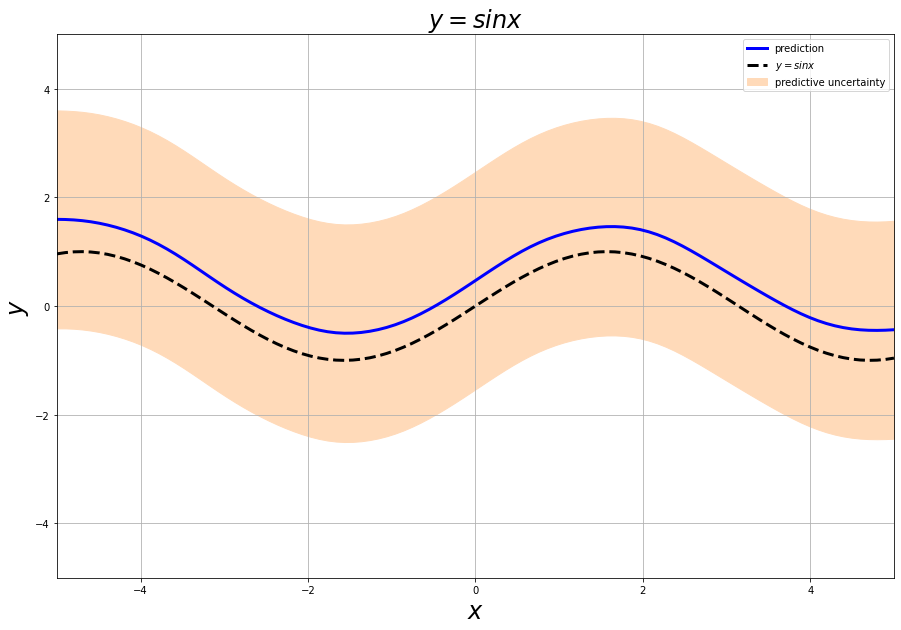
\includegraphics[width=\textwidth]{nll/near_large}
	\caption{Close prediction with high uncertainty}
	\label{fig_1d_functions_nll0}
\end{subfigure}
\hfill
\begin{subfigure}[b]{0.3\textwidth}
	\centering
	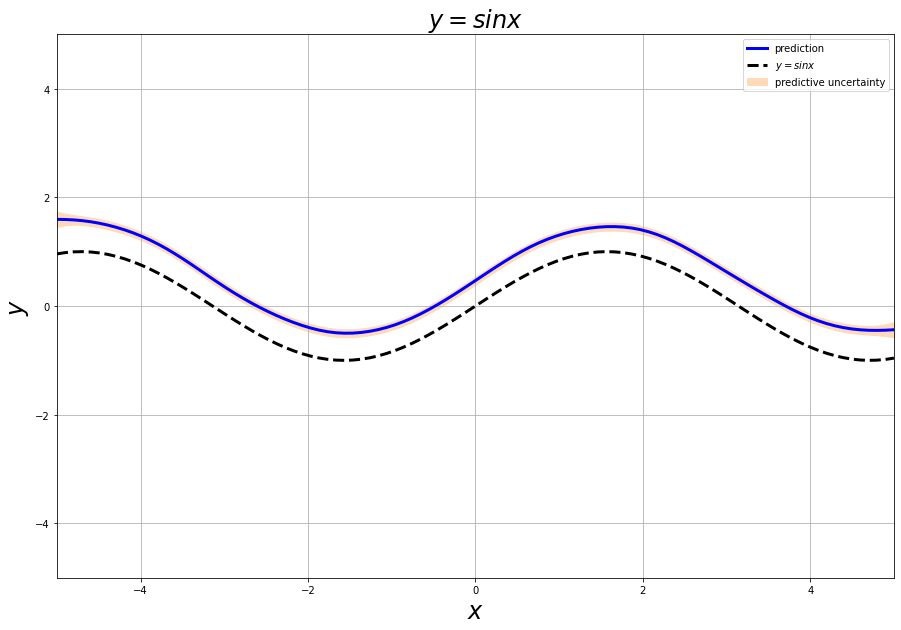
\includegraphics[width=\textwidth]{nll/near_small}
	\caption{Close prediction with low uncertainty}
	\label{fig_1d_functions_nll1}
\end{subfigure}
\hfill
\begin{subfigure}[b]{0.3\textwidth}
	\centering
	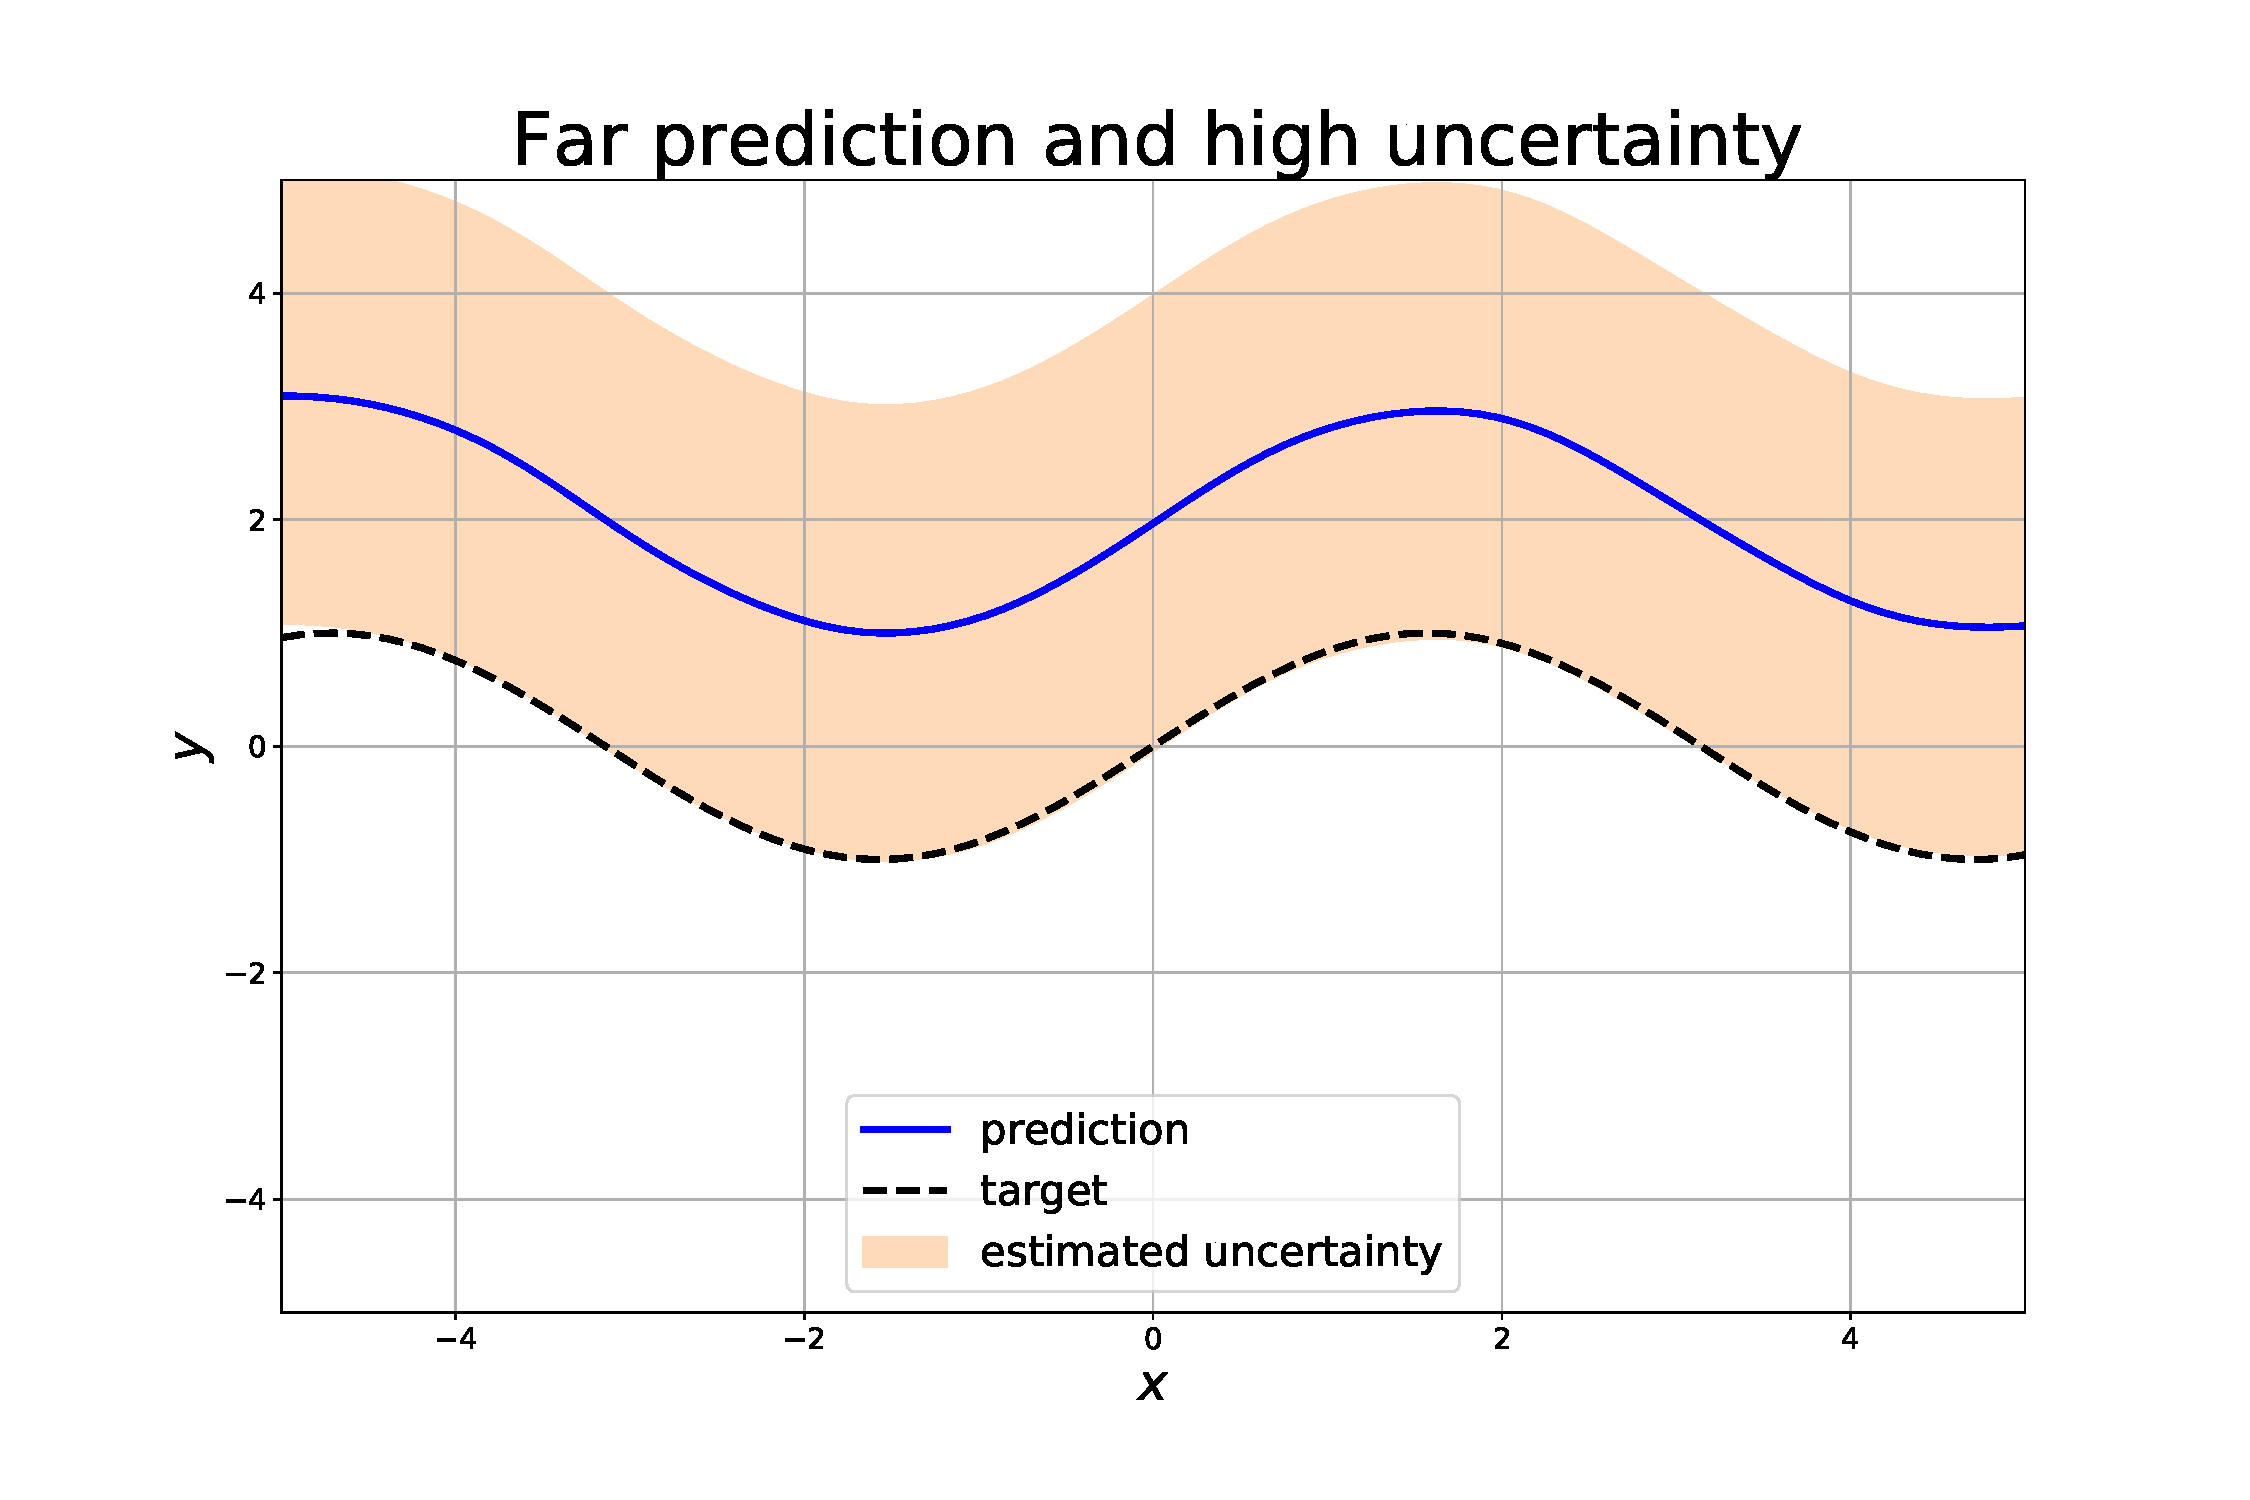
\includegraphics[width=\textwidth]{nll/far_large}
	\caption{Far prediction with high uncertainty}
	\label{fig_1d_functions_nll2}
\end{subfigure}
\hfill
\begin{subfigure}[b]{0.3\textwidth}
	\centering
	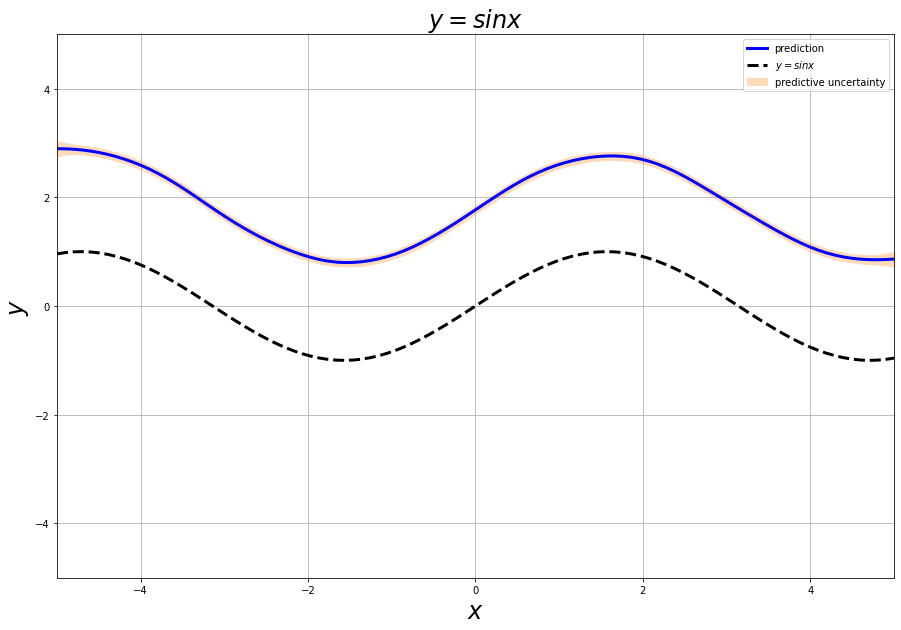
\includegraphics[width=\textwidth]{nll/far_small}
	\caption{Far prediction with low uncertainty}
	\label{fig_1d_functions_nll3}
\end{subfigure}
\hfill
\caption{Plots to explain effects of predictions and confidence bounds on NLL }
\label{fig_1d_functions_nll}
\end{figure}
\begin{table}[H]
	\centering
	\begin{tabular}{|l|l|l|l|}
		\hline
		\multicolumn{1}{|c|}{\textbf{Case}}                                               & \multicolumn{1}{c|}{\textbf{NLL}} & \multicolumn{1}{c|}{\textbf{RMSE}} & \textbf{EVA} \\ \hline
		\begin{tabular}[c]{@{}l@{}}Close prediction \\ with high uncertainty\end{tabular} & 1.04                              & 0.50                               & 0.99         \\ \hline
		\begin{tabular}[c]{@{}l@{}}Close prediction \\ with low uncertainty\end{tabular}  & 87.46                             & 0.50                               & 0.99         \\ \hline
		\begin{tabular}[c]{@{}l@{}}Far prediction \\ with high uncertainty\end{tabular}   & 4.05                              & 2.50                               & 0.99         \\ \hline
		\begin{tabular}[c]{@{}l@{}}Far prediction \\ with low uncertainty\end{tabular}    & 2220.67                           & 2.50                               & 0.99         \\ \hline
	\end{tabular}
\caption{Different cases to describe the impact of prediction distance and uncertainty levels on metrics}
\label{tab_nll_cases}
\end{table}
NLL measures the goodness of fit of the approximated posterior distribution to the true function's mean(ground truth). The metric fails to evaluate fidelity of the approximated posterior distribution. Therefore, NLL \enquote{may be a good criteria for model
selection, it is not a reliable criteria for determining how well an approximate posterior aligns with the true posterior}\cite{yao2019quality}. 
Plots in the Figure \ref{fig_1d_functions_nll} depict different possible cases of predictions and uncertainty levels whose corresponding NLL, RMSE and EVA values are tabulated in \ref{tab_nll_cases}. It can be inferred from \ref{fig_1d_functions_nll0} and  \ref{fig_1d_functions_nll1} that irrespective of both predictions being identical, width of confidence intervals has a huge impact on their NLL values. Likewise, the prediction in \ref{fig_1d_functions_nll1} is much closer to the target than the one in \ref{fig_1d_functions_nll2}, yet the former is penalized heavily in terms of NLL(2220.67) due to its low value of uncertainty. However, values of EVA remain constant for all scenarios and RMSE changes only when there is a shift in the prediction. This signifies that the interpretation of NLL as a metric for uncertainty estimation quality holds good only when it is considered along with a measure of predictive accuracy like RMSE. Also, the metric can be used to compare methods only when they are evaluated on the same dataset.

\vfill\section{Predictive accuracy and uncertainty quality}
\subsubsection{\textbf{RQ2.} How do the identified uncertainty estimation methods compare with each other and Gaussian Process models, based on their uncertainty estimation quality and prediction accuracy of their respective models?}
\subsection{Udacity steering angle dataset}
\subsubsection{Quantitative comparison}

\begin{table}[H]
	\centering
	\begin{tabular}{|c|c|c|c|}
		\hline
		\multirow{2}{*}{\textbf{Model}}                                                                             & \multirow{2}{*}{\textbf{RMSE}}      & \multirow{2}{*}{\textbf{EVA}} & \multirow{2}{*}{\textbf{NLL}} \\
		&                                     &                               &                               \\ \hline
		Vanilla Dronet                                                                                              & 0.034                               & 0.98                          & NA                            \\ \hline
		MCDO\_ADF Dronet                                                                                            & 0.151                                & 0.68                 & -0.74                         \\ \hline
		\begin{tabular}[c]{@{}c@{}}Evidential Dronet\\ (squared version of loss)\end{tabular}                       & 0.022                               & \bf{0.99}                          & \textbf{-0.94}                \\ \hline
		\multicolumn{1}{|l|}{\begin{tabular}[c]{@{}l@{}}Evidential Dronet\\ (L1 norm version of loss)\end{tabular}} & \multicolumn{1}{l|}{\textbf{ 0.021}} & \multicolumn{1}{l|}{\textbf{0.99}}     & \multicolumn{1}{l|}{0.31}     \\ \hline
	\end{tabular}
	\caption{A quantitative comparison of uncertainty estimation methods when applied to Dronet}
\label{tab_quant_compare}
\end{table}

\begin{itemize}
	\item It can be inferred that Evidential Dronet outperforms the other two models in terms of both predictive accuracy and quality of uncertainty estimation(NLL).
	\item In the case of predictive accuracy expressed in terms of RMSE, Evidential Dronet outperforms the Vanilla variant only by a slight margin. However, difference in RMSE between Evidential and MCDO\_ADF variants is considerable. This could be partly attributed to the fact that both predictions and uncertainty estimates outputted by the MCDO\_ADF variant depend on the count of Monte-Carlo(MC) samples considered. Higher the value of MC samples better the model's performance(refer Figure \ref{fig_mc_count_vs_rmse}).  However, this holds true only un till a particular value of MC samples. For this experiment, 20 MC samples are considered. 
	\item The relationship between MC sample counts and predictive accuracy holds good for the Explained Variance (EVA) measure as well.
	\item The quality of predictive uncertainty estimated by the Evidential Dronet expressed in terms of Negative-Log-Likelihood (NLL) is better than the MCDO\_ADF variant. This intuitively means that the former technique is able to determine parameters of the distribution in which likelihood of finding ground truth labels is higher than in the distribution outputted by the latter.
\end{itemize}
\begin{figure}[H]
	\centering
	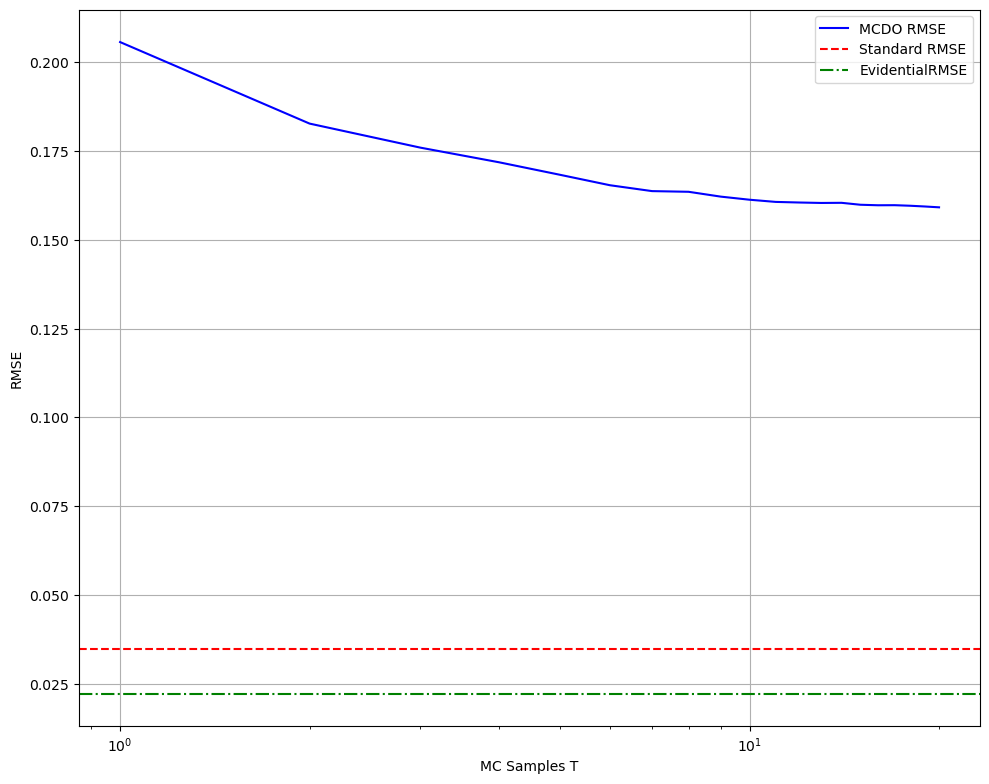
\includegraphics[scale=0.5]{RMSE_T20}
	\caption{Plot depicting relationship between the MC sample count and RMSE during the MCDO\_ADF model inference}
	\label{fig_mc_count_vs_rmse}
\end{figure}
\begin{figure}[H]
	\centering
	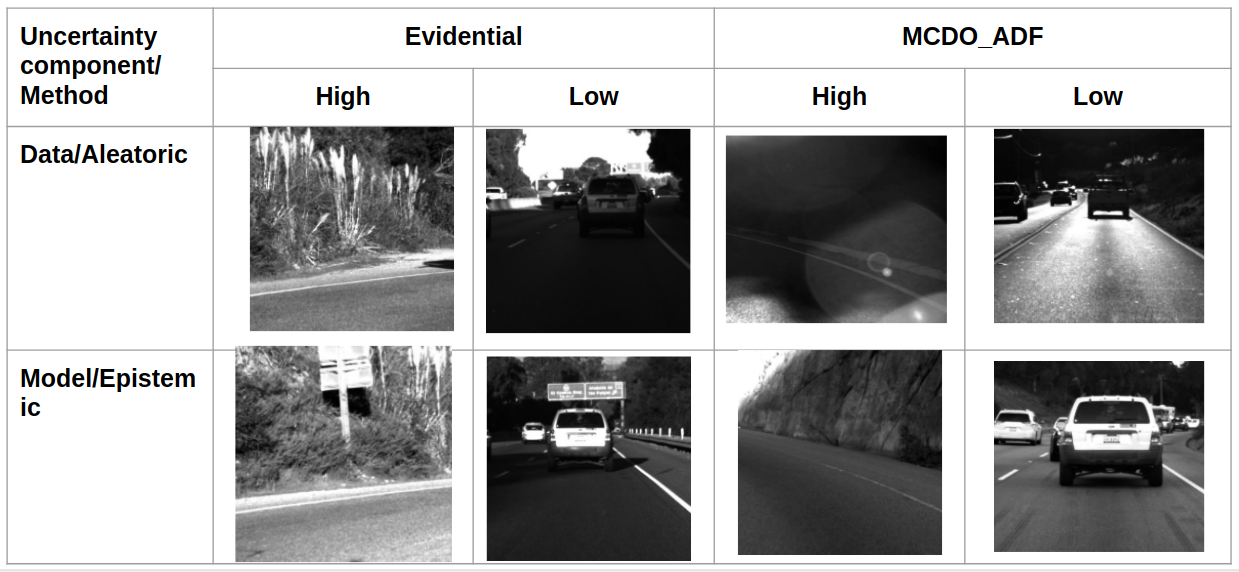
\includegraphics[scale=0.4]{uncertainty_extremes}
	\caption{A set of sample images with extreme levels of uncertainties predicted by both the methods}
	\label{fig_uncertainty_extremes}
\end{figure}
\subsubsection{Qualitative comparison}
\begin{table}[H]
\begin{tabular}[h]{|p{1.5cm}|p{2.3cm}|p{12.5cm}|}
\hline
\textbf{Category}&\textbf{Method}&\textbf{Analysis}\\
\hline
Aleatoric&MCDO\_ADF&\begin{itemize}\item The method performs well in estimating data uncertainty.The presence of glare, blur, and poor illumination in images reported with high values show that the estimated uncertainty is indeed aleatoric. \item Most of the images reported with low values of aleatoric uncertainty are characterized by high contrast and low noise levels. \item There also exist certain over-illuminated images for which the method reports a low value of data-uncertainty and is undesirable.\end{itemize}\\
\hline
Aleatoric&DER/Evidential&\begin{itemize}\item The method reports a high-value of aleatoric uncertainty for blurry and unclear images and is desirable.\item  It is interesting to note that this method reports high-values of data uncertainty for images with objects such as grass that produce patterns similar to noise.\item Similar to MCDO\_ADF this method performs well in reporting low aleatoric uncertainty for clear images except for the ones with shadows.\end{itemize}\\
\hline
Epistemic&MCDO\_ADF&\begin{itemize}\item The method reports high values of epistemic uncertainty for both images with unclear lane markings(intuitively a key feature to predict steering angles) and noise induced by factors such as blur and glare.\item Reporting high values of epistemic uncertainty for noisy images proves the method's ability to jointly model both the components of uncertainty.\item Similar to the aleatoric case, the method reports low values of epistemic uncertainty for clear images except for the ones with poor and over illumination.\end{itemize}\\
\hline
Epistemic&DER/Evidential&\begin{itemize}\item The method produces high values of model uncertainty for both images with unclear features and noise, similar to MCDO\_ADF.\item However, there is a difference between images reported with high values of epistemic uncertainty between MCDO\_ADF and evidential showing the fact that they both have different criteria for uncertainty estimation.\item The set of images reported with low values of epistemic uncertainty have a lot of similarities with that of ones with low-aleatoric variances.\end{itemize}\\
\hline
Total& MCDO\_ADF and DER/Evidential& The set of images reported with high/low values of predictive uncertainties by both the methods correspond to the ones with high/low values of their components(aleatoric and epistemic)\\
\hline
\end{tabular}
\caption{A qualitative comparison of uncertainty estimation methods}
\label{tab_qualit_compare}
\end{table}
\end{document}

\subsection{1D dataset}
\begin{table}[H]
	\begin{tabular}{|c|c|c|c|c|c|}
		\hline
		\textbf{\begin{tabular}[c]{@{}c@{}}Function\\ y=f(x)\end{tabular}} & \textbf{Metric} & \textbf{\begin{tabular}[c]{@{}c@{}}Homoscedastic\\ GP\end{tabular}} & \textbf{\begin{tabular}[c]{@{}c@{}}Heteroscedastic\\ GP\end{tabular}} & \textbf{Evidential} & \textbf{MCDO\_ADF}                    \\ \hline
		\multirow{3}{*}{$y=\frac{sin(3x)}{3x}$}                            & NLL             & \textbf{-0.82}                                                      & -0.51                                                                 & \textit{0.57}                & 2.27                                  \\ \cline{2-6} 
		& RMSE            & \textbf{0.07}                                                       & 0.08                                                                  & 0.40                & \textit{0.39}                                  \\ \cline{2-6} 
		& EVA             & \textbf{0.94}                                                       & 0.91                                                                  & \textit{-0.29 }              & -0.43                                 \\ \hline
		\multirow{3}{*}{$y=0.1x^3$}                                        & NLL             & \textbf{-2.44}                                                      & -1.77                                                                 & -\textit{0.15}               & 1.11                                  \\ \cline{2-6} 
		& RMSE            & \textbf{0.01}                                                 & 0.03                                                                  & 0.23                & \textit{0.11 }                                 \\ \cline{2-6} 
		& EVA             & \textbf{0.99}                                                                & \textbf{0.99}                                                                  & \textbf{0.99}       & \textbf{0.99}                                  \\ \hline
		\multirow{3}{*}{$y=-(1+x)sin(1.2x)$}                               & NLL             & \textbf{-1.02}                                                      & 1.91                                                                  & \textit{6.14}                & \textgreater{}\textgreater{}1(182049) \\ \cline{2-6} 
		& RMSE            & 0.61                                                                & \textbf{0.15}                                                         & 2.68                & \textit{0.8}                                   \\ \cline{2-6} 
		& EVA             & 0.94                                                                & \textbf{0.99}                                                         & \textit{-0.05}               & 0.87                                  \\ \hline
	\end{tabular}
	\caption{A quantitative comparison of uncertainty estimation methods on 1D datasets}
	\label{tab_quant_compare1D}
\end{table}

\begin{itemize}
	\item It can be inferred from the tabulation that Gaussian processes outperform the considered pair of uncertainty estimation methods in terms of every metric(values marked in bold). However, the pair GP models are included in this comparison only as a baseline.
	\item When it comes to comparing DER with MCDO(italicized values correspond to better performance), the former performs better in terms of NLL and EVA while the latter has relatively lower values of RMSE, the measure of predictive accuracy.
	\item Better performance of DER over MCDO\_ADF can be attributed to three important factors:
	\begin{itemize}
		\item Flexibility: The extent of confidence interval around a prediction estimated by a method.
		\item Quality of model fit to data
		\item Performance in Out-Of-Distribution regions(discussed more in the next section).
	\end{itemize}
	\item MCDO\_ADF suffers from high values of NLL (undesirable) in case of all the three functions due to lack of flexibility.
\end{itemize}
\subsubsection{Qualitative comparison}\label{sec_qual_comparison}
\begin{itemize}
	\item As it can be witnessed from \ref{der_fn1},\ref{der_fn2} and \ref{der_fn3} DER provides a constant estimate for the value of aleatoric uncertainty similar to homoscedastic GP, which is desirable. 
	\item The MCDO\_ADF technique  performs relatively better than DER in estimating epistemic uncertainties for fn\_1(refer \ref{mcdo_fn1}), while its performance plummets in the case of fn\_3(refer \ref{mcdo_fn3}) where it fails to report high values of uncertainty for the OOD region which results in a very high value of NLL.
	\item The MCDO\_ADF variant of the neural network model performs better than its DER counterpart in modeling smoothness of functions. While in the case of GPs, the use of squared-exponential kernels as priors leads to better modeling of such functions.  
	\item The success of homoscedastic GPs in modeling  aleatoric uncertainties can be attributed to constancy in variance of Gaussian distribution used for adding noise to input data generated from a given function. 
	
	
\end{itemize}
\begin{figure}[H]
	\centering
	\begin{subfigure}[b]{0.4\textwidth}
		\centering
		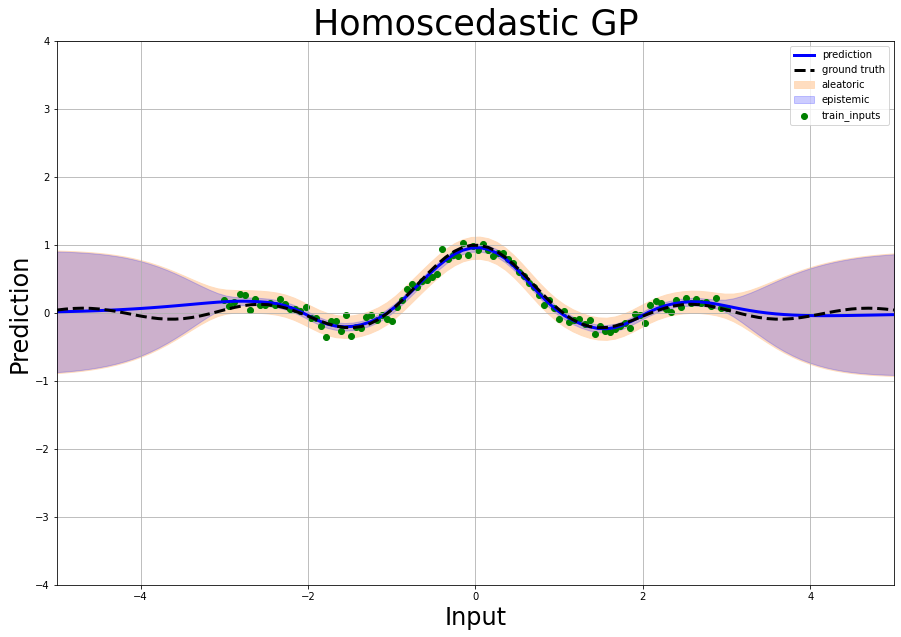
\includegraphics[width=\textwidth]{toy_dataset/homo_fn1}
		\caption{Homoscedastic GP on fn\_1: $y=\frac{sin(3x)}{3x}$}
		\label{homo_fn1}
	\end{subfigure}
	\hfill
	\begin{subfigure}[b]{0.4\textwidth}
		\centering
		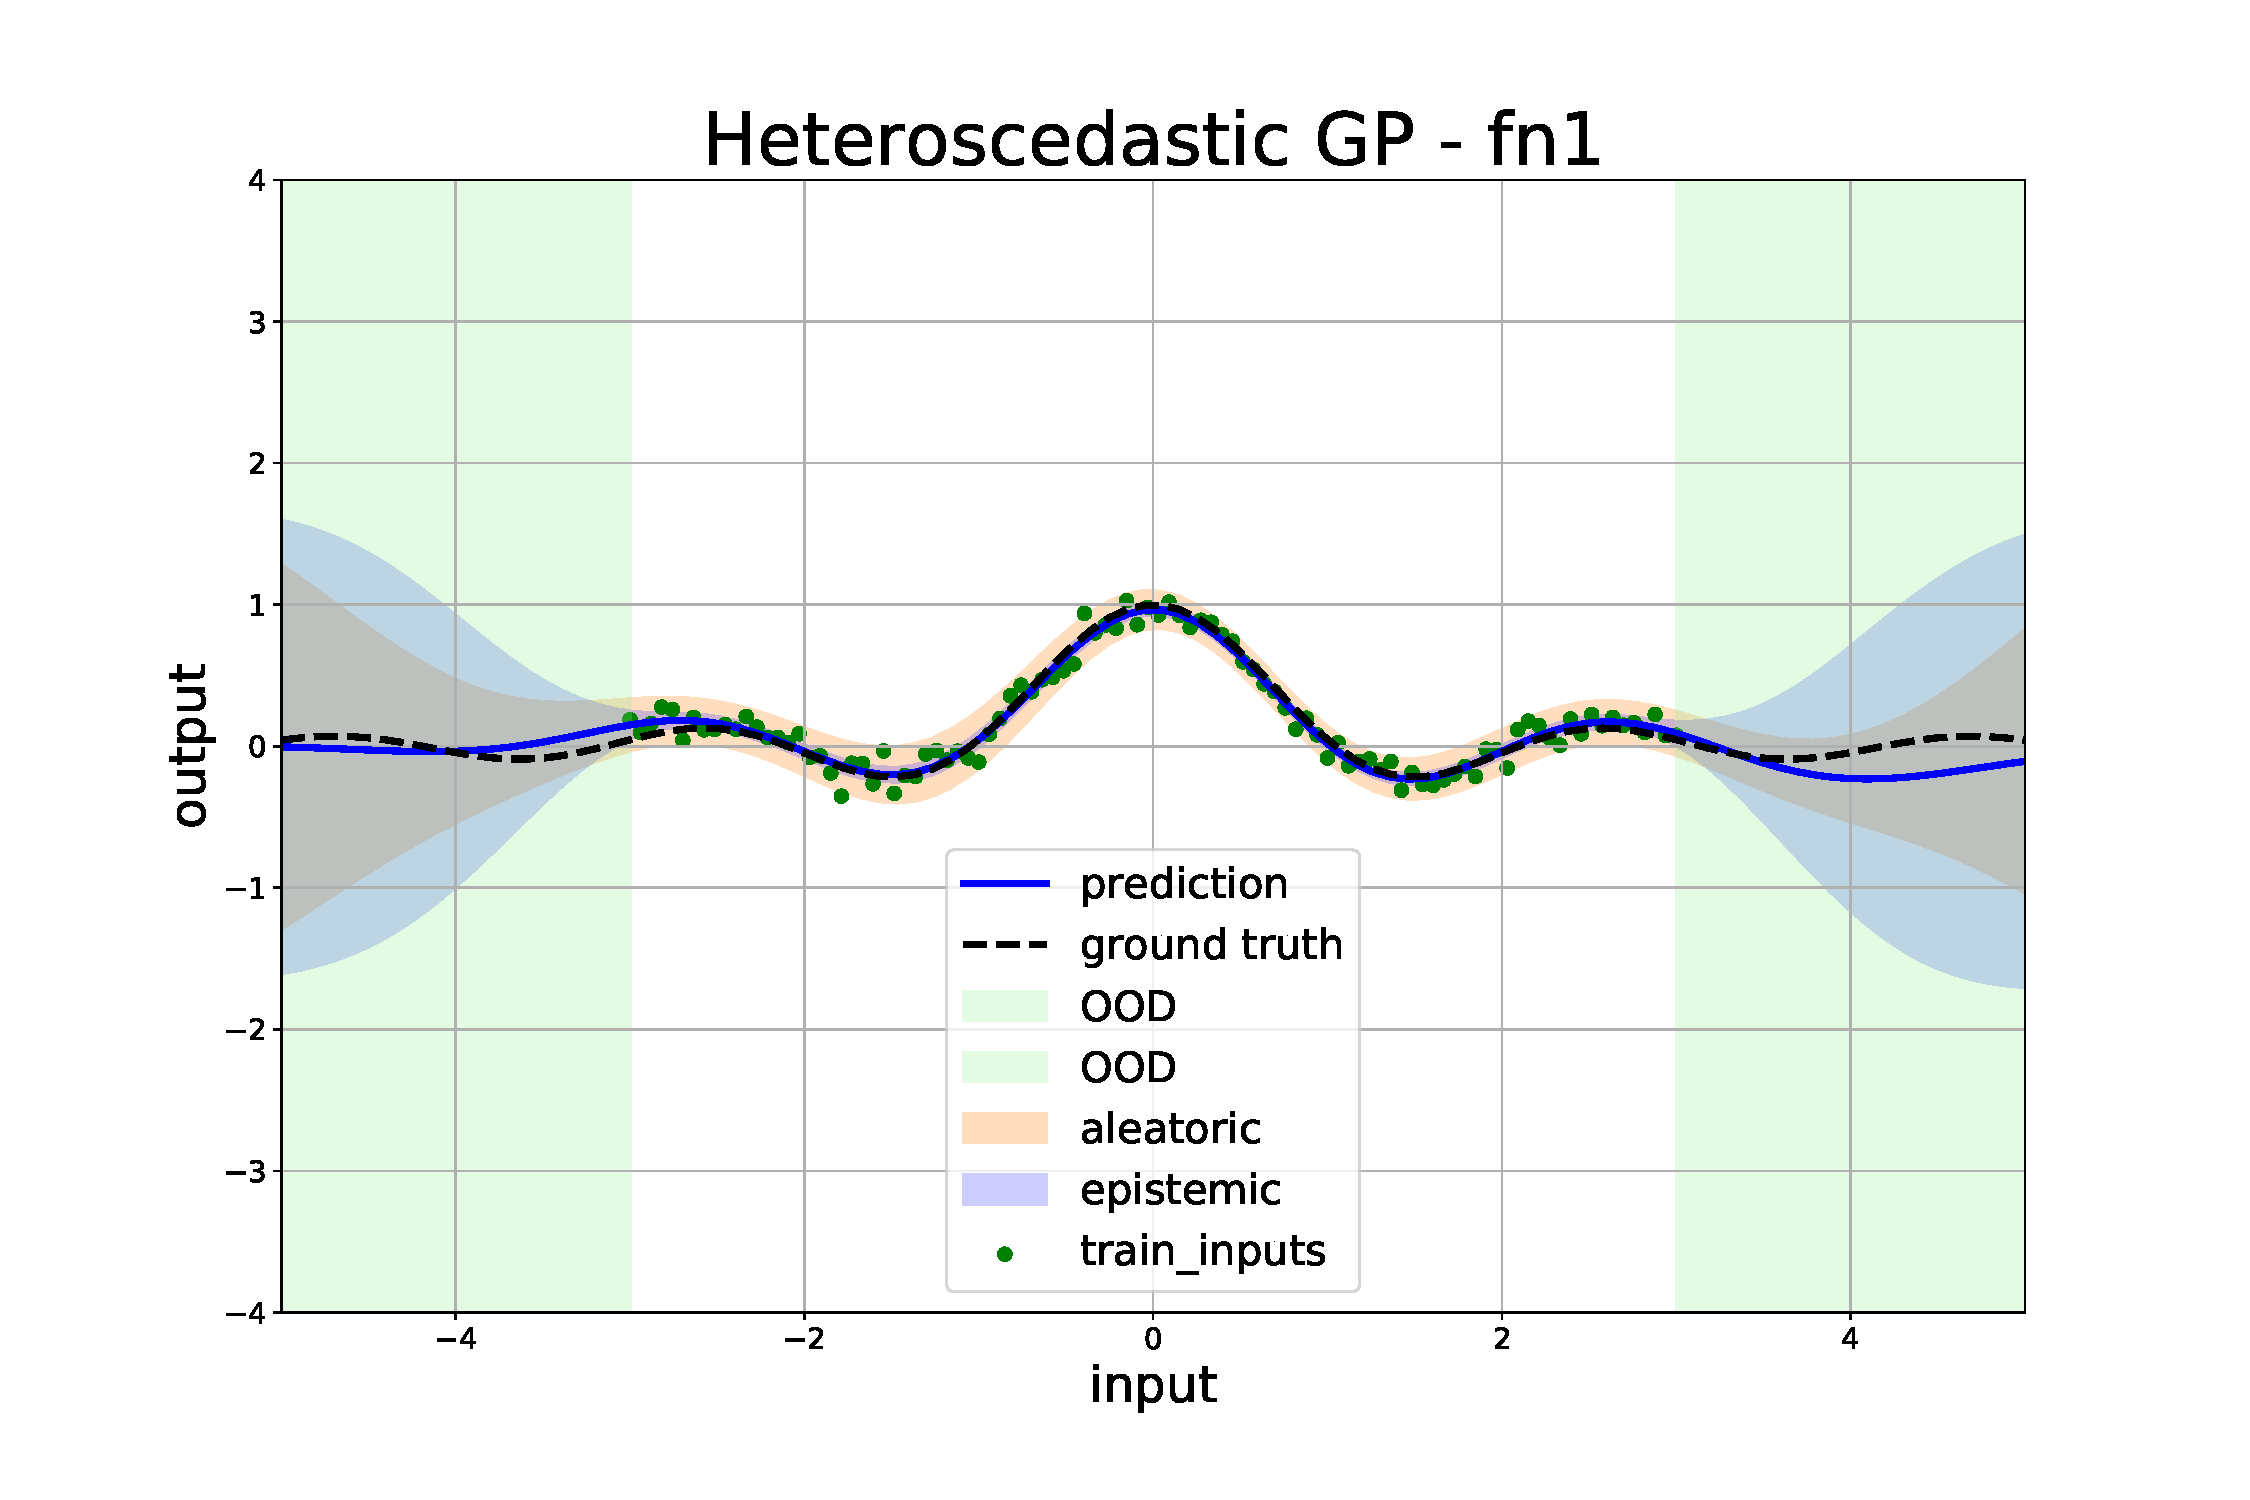
\includegraphics[width=\textwidth]{toy_dataset/hetero_fn1}
		\caption{Heteroscedastic GP on fn\_1: $y=\frac{sin(3x)}{3x}$}
		\label{hetero_fn1}
	\end{subfigure}
	\hfill
	\begin{subfigure}[b]{0.4\textwidth}
		\centering
		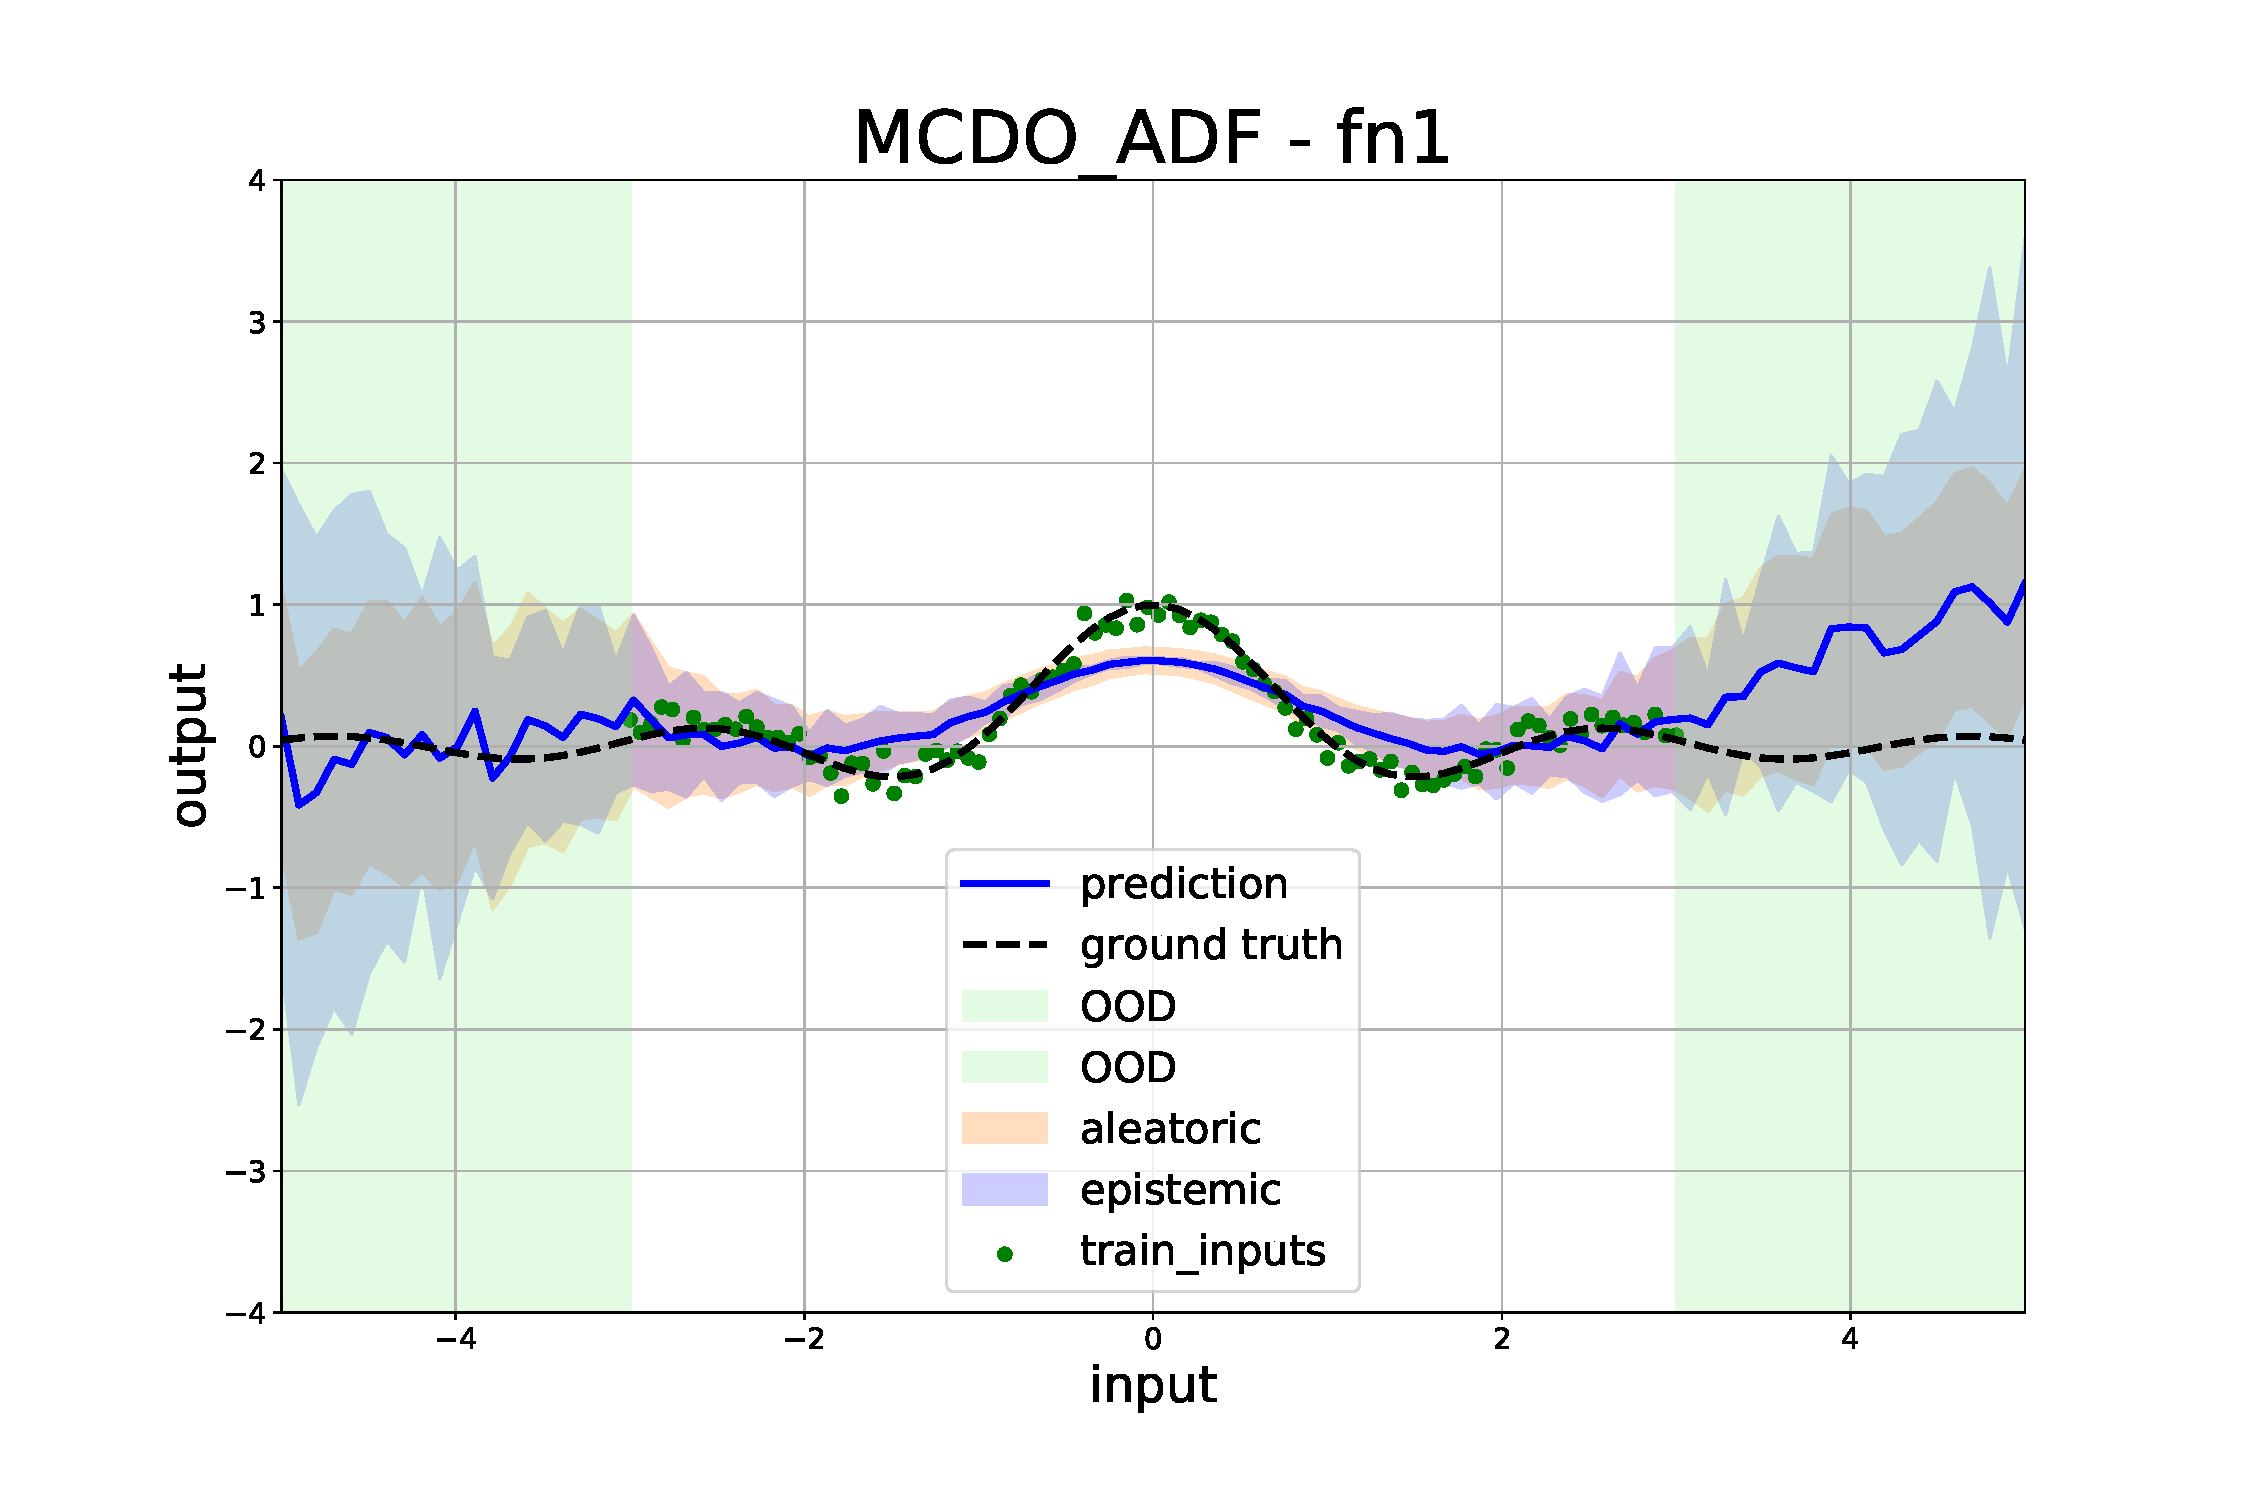
\includegraphics[width=\textwidth]{toy_dataset/mcdo_fn1}
		\caption{MCDO\_ADF on fn\_1: $y=\frac{sin(3x)}{3x}$}
		\label{mcdo_fn1}
	\end{subfigure}
	\hfill
	\begin{subfigure}[b]{0.4\textwidth}
		\centering
		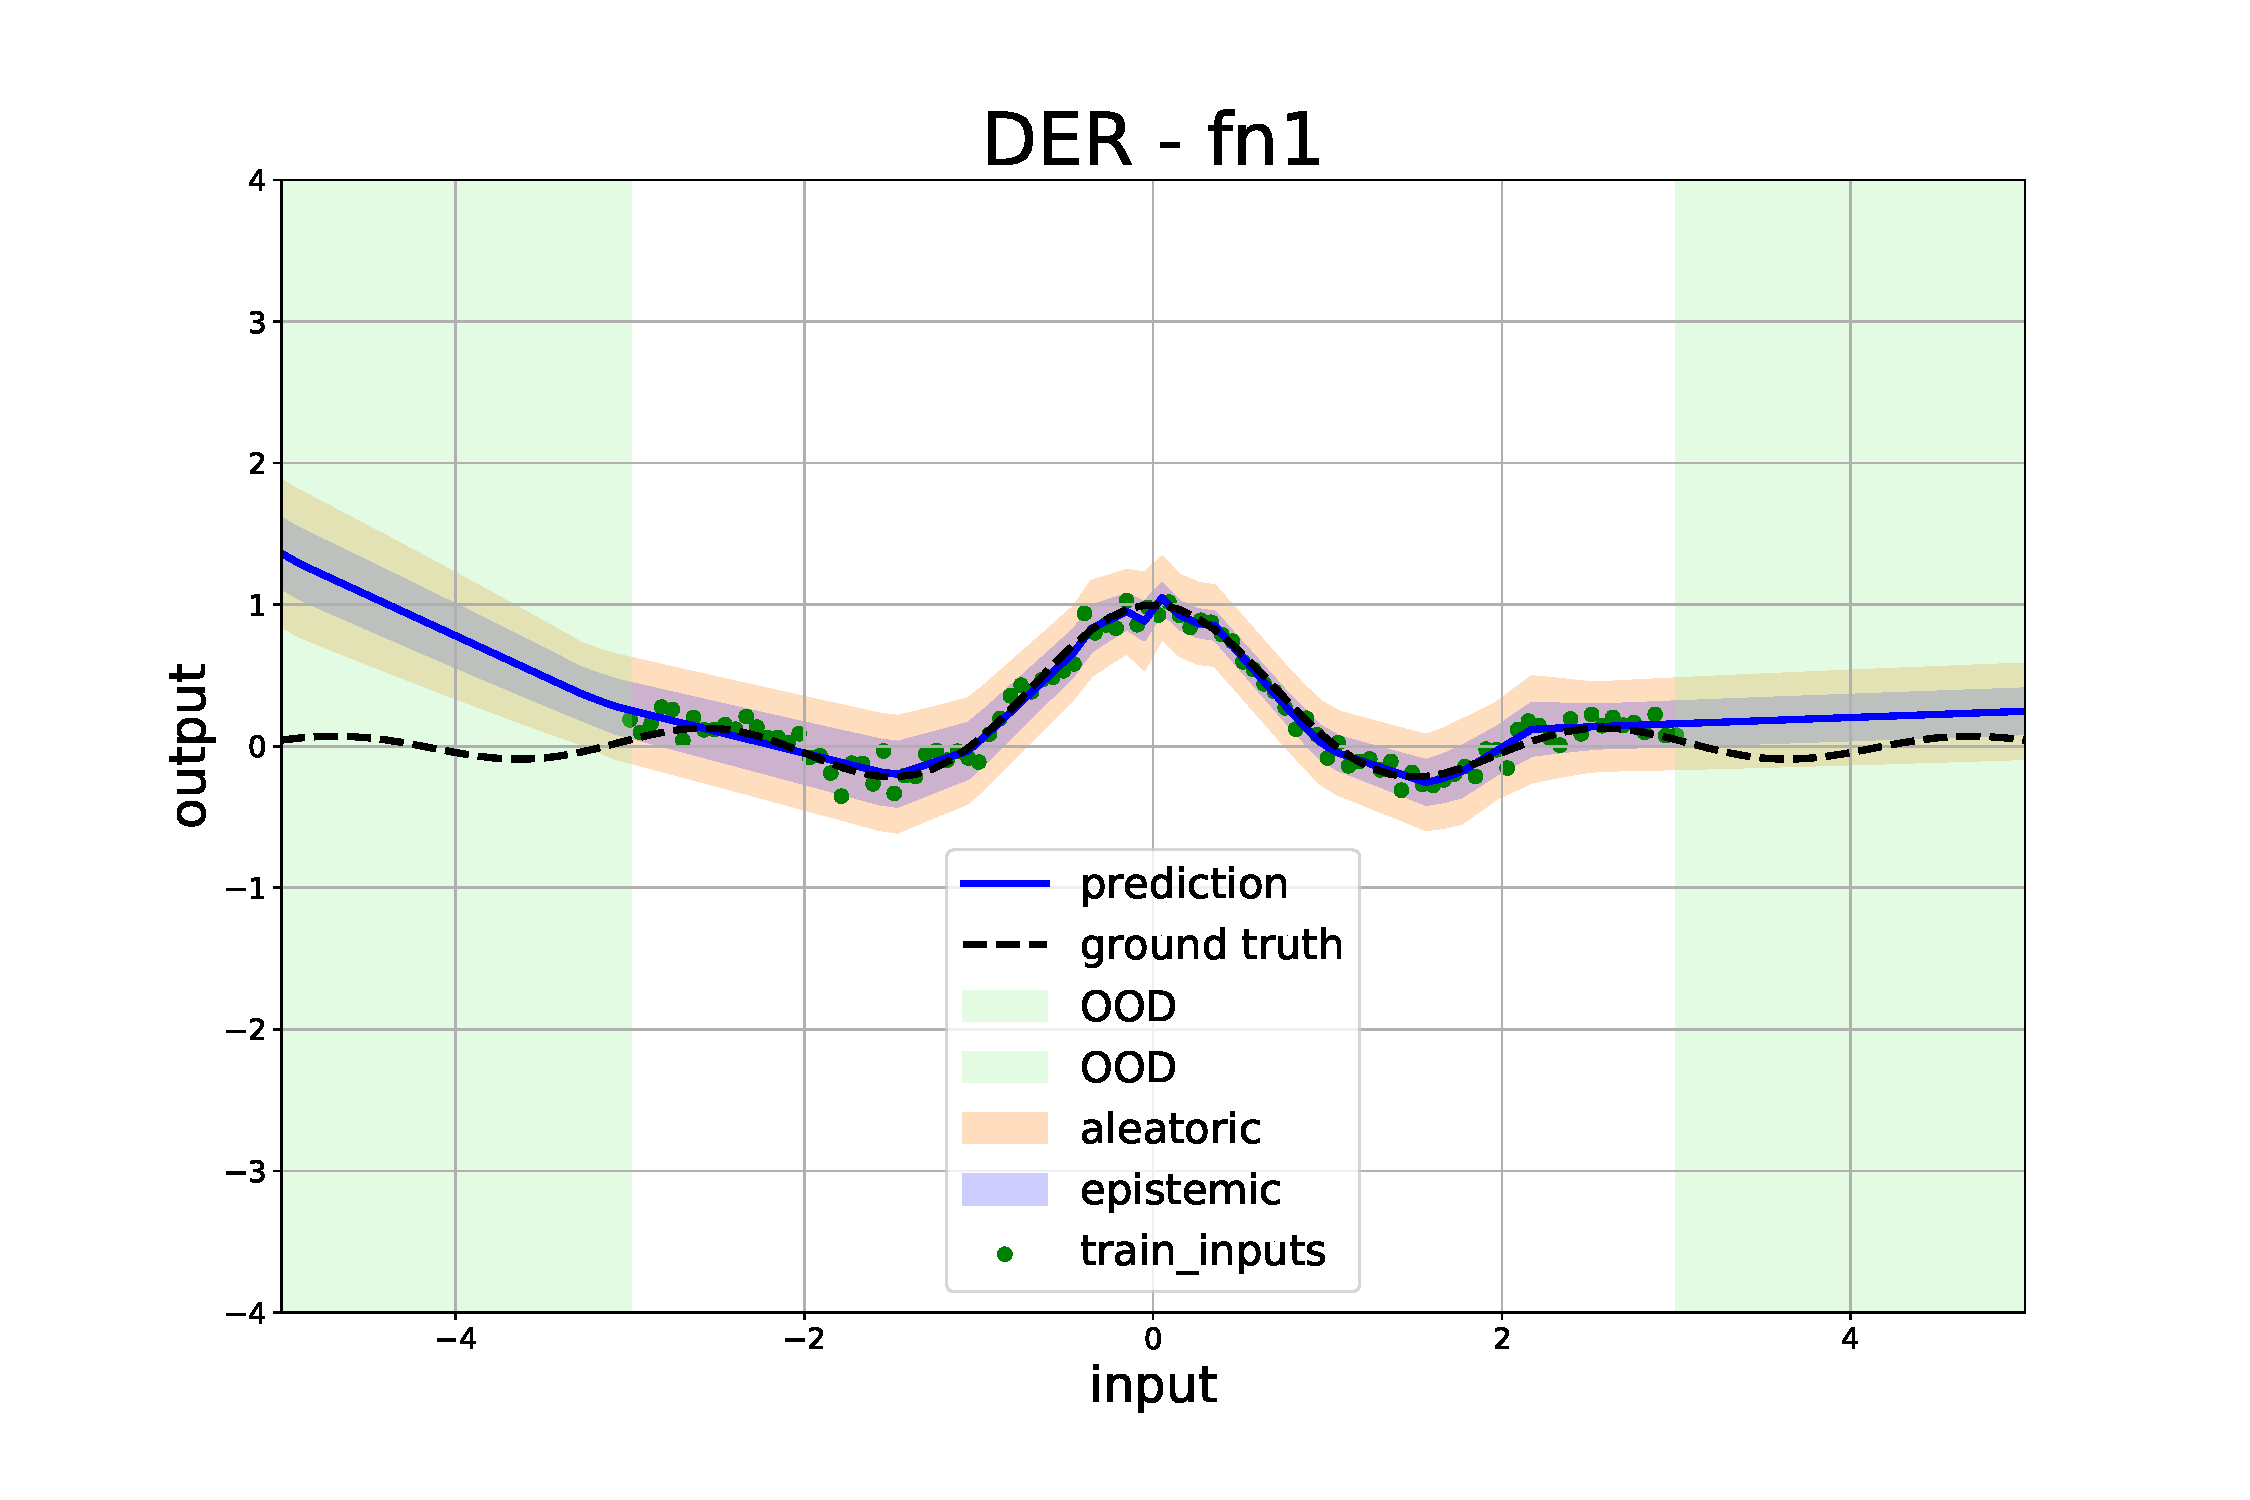
\includegraphics[width=\textwidth]{toy_dataset/der_fn1}
		\caption{DER on fn\_1: $y=\frac{sin(3x)}{3x}$}
		\label{der_fn1}
	\end{subfigure}
	\hfill
	\begin{subfigure}[b]{0.4\textwidth}
		\centering
		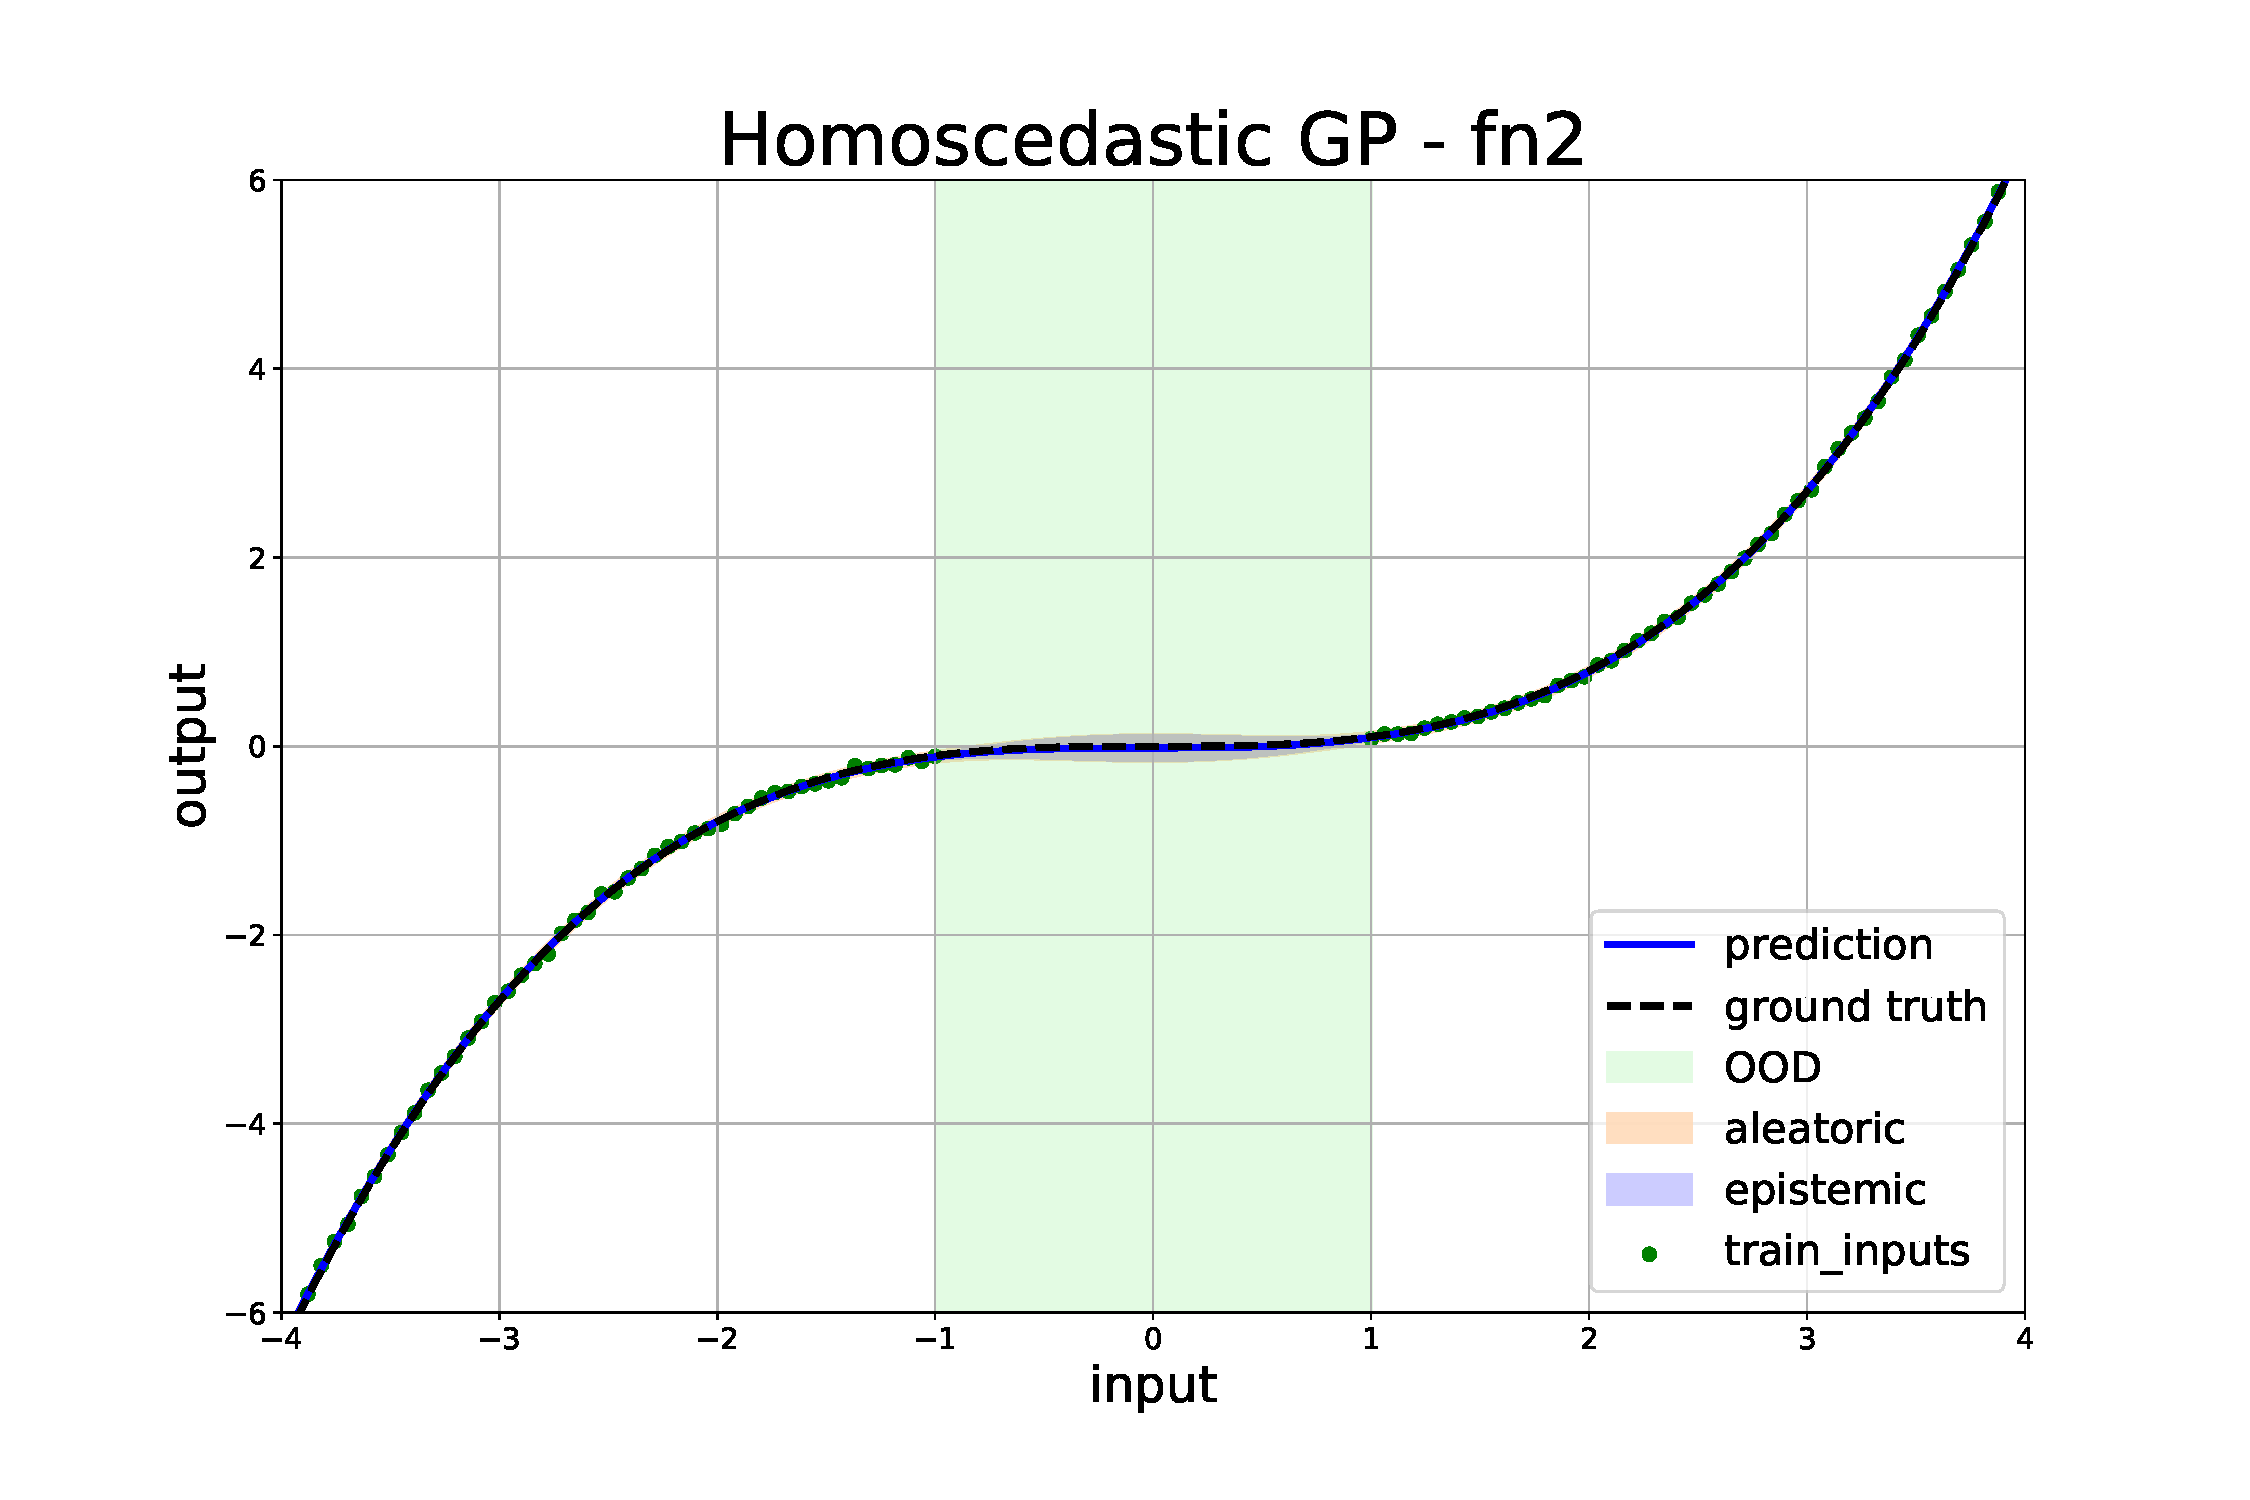
\includegraphics[width=\textwidth]{toy_dataset/homo_fn2}
		\caption{Homoscedastic GP on fn\_2: $y=0.1x^3$}
		\label{homo_fn2}
	\end{subfigure}
	\hfill
	\begin{subfigure}[b]{0.4\textwidth}
		\centering
		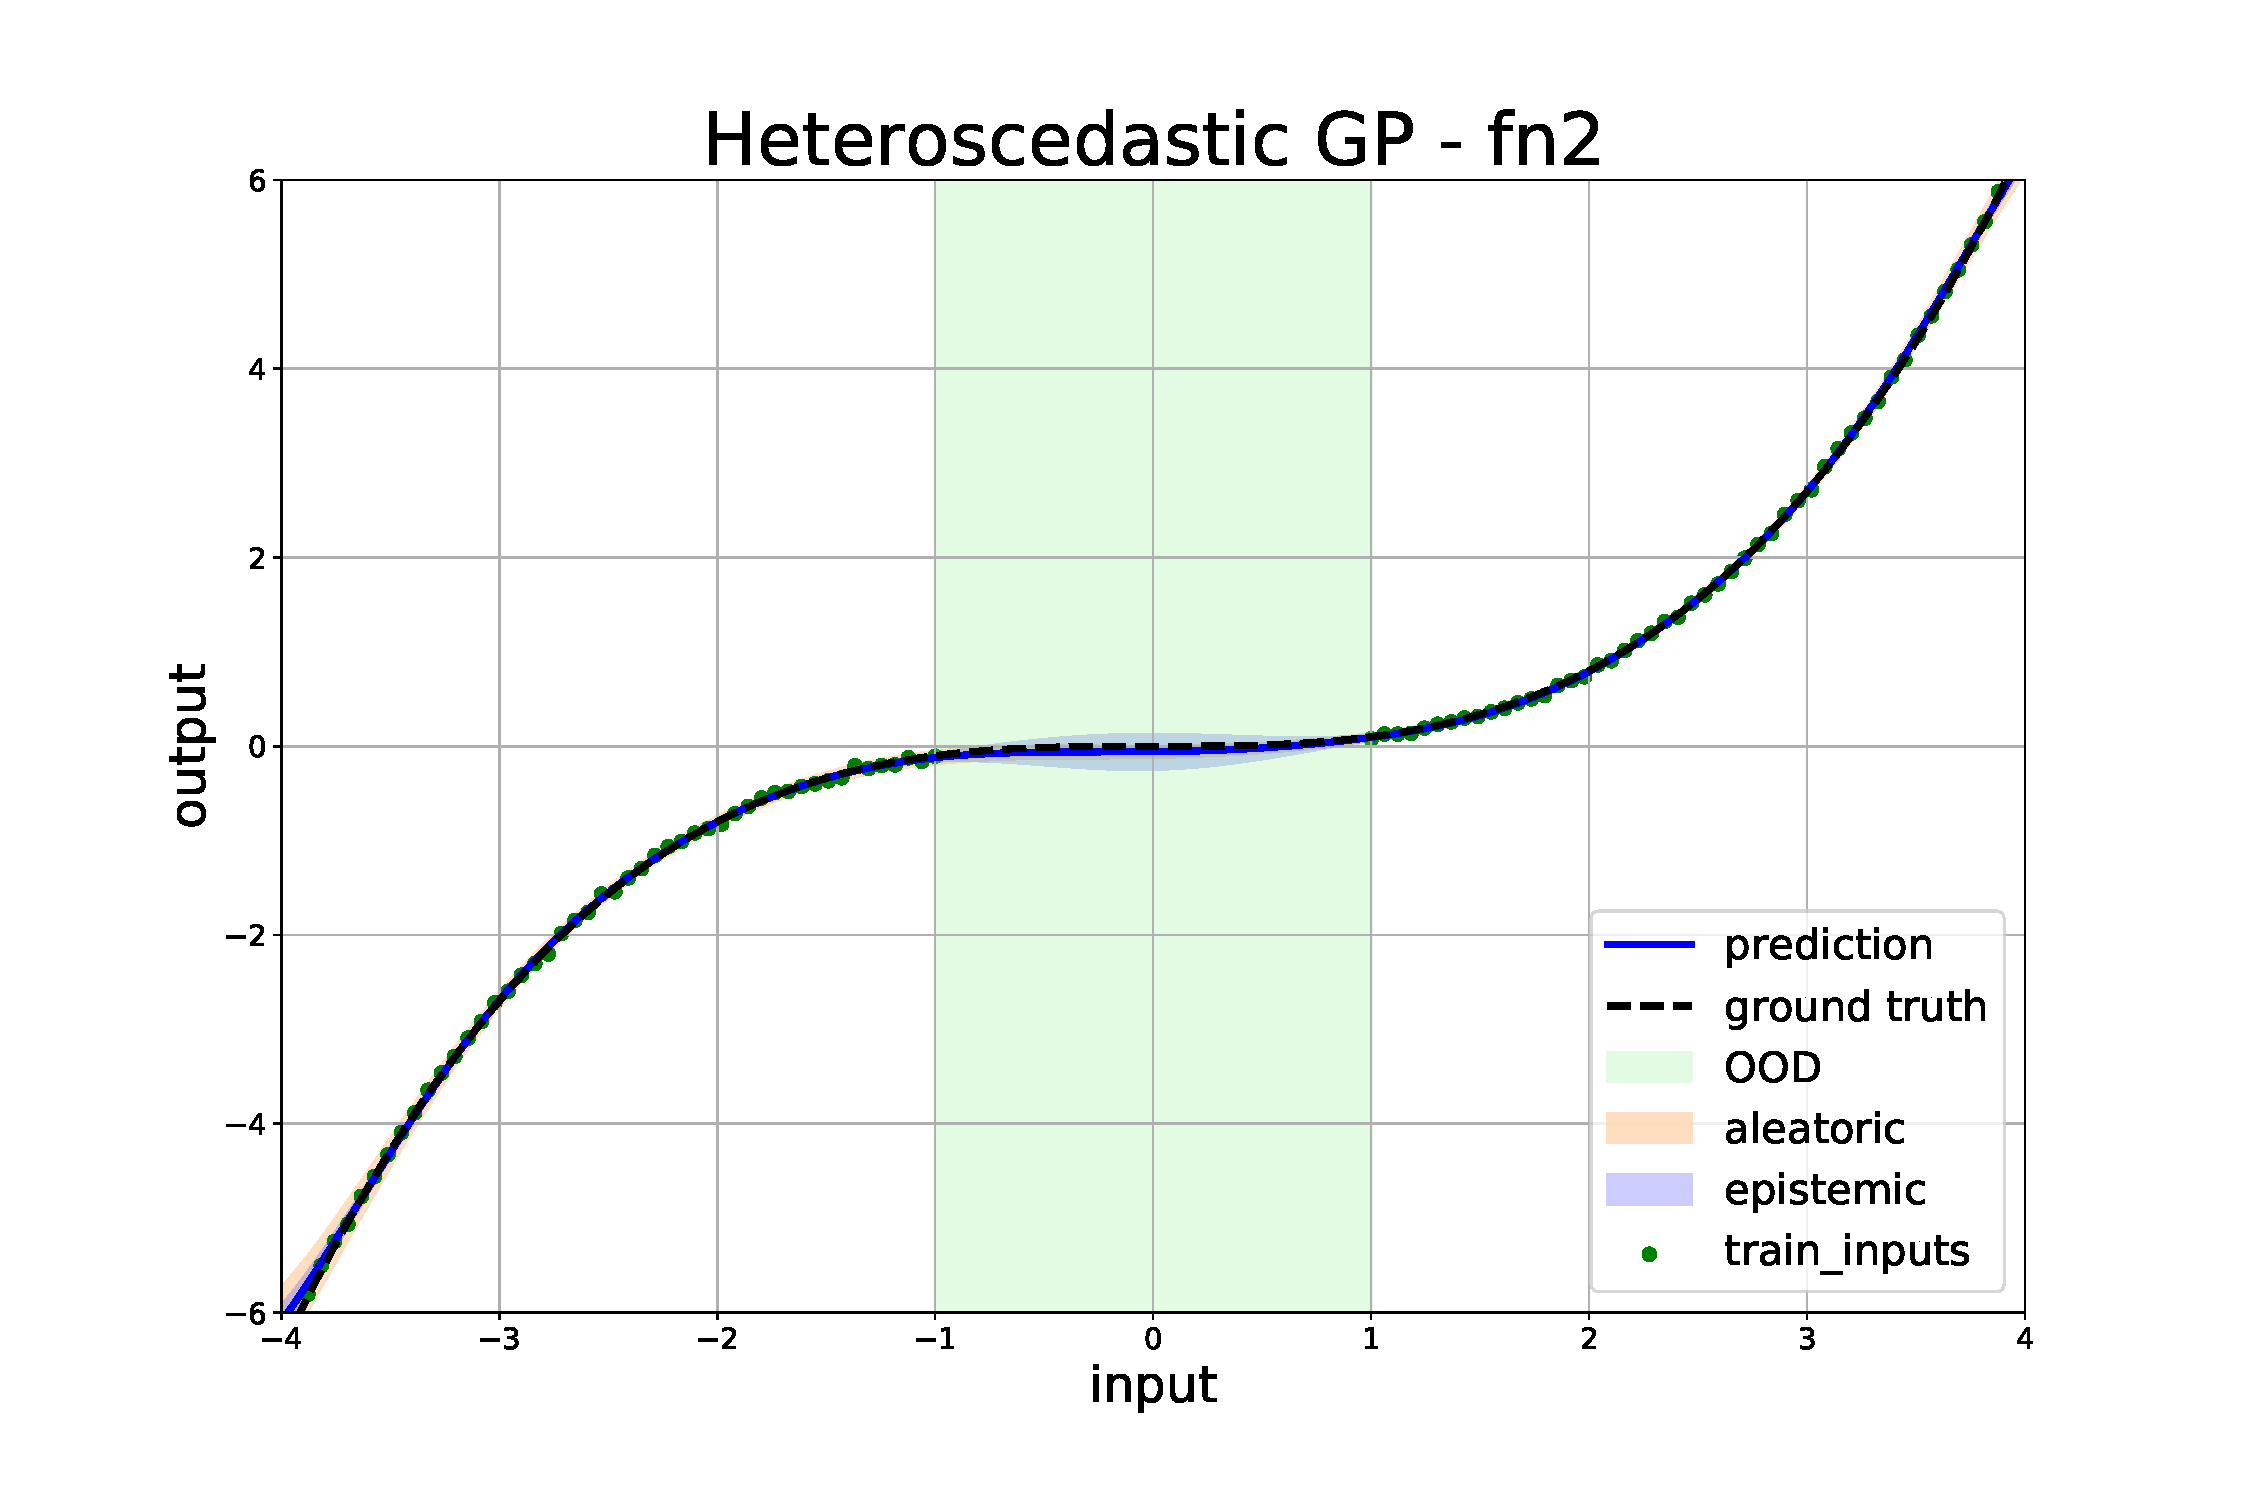
\includegraphics[width=\textwidth]{toy_dataset/hetero_fn2}
		\caption{Heteroscedastic GP on fn\_2: $y=0.1x^3$}
		\label{hetero_fn2}
	\end{subfigure}
\end{figure}

\begin{figure}[H]\ContinuedFloat
	\centering
	\begin{subfigure}[b]{0.4\textwidth}
		\centering
		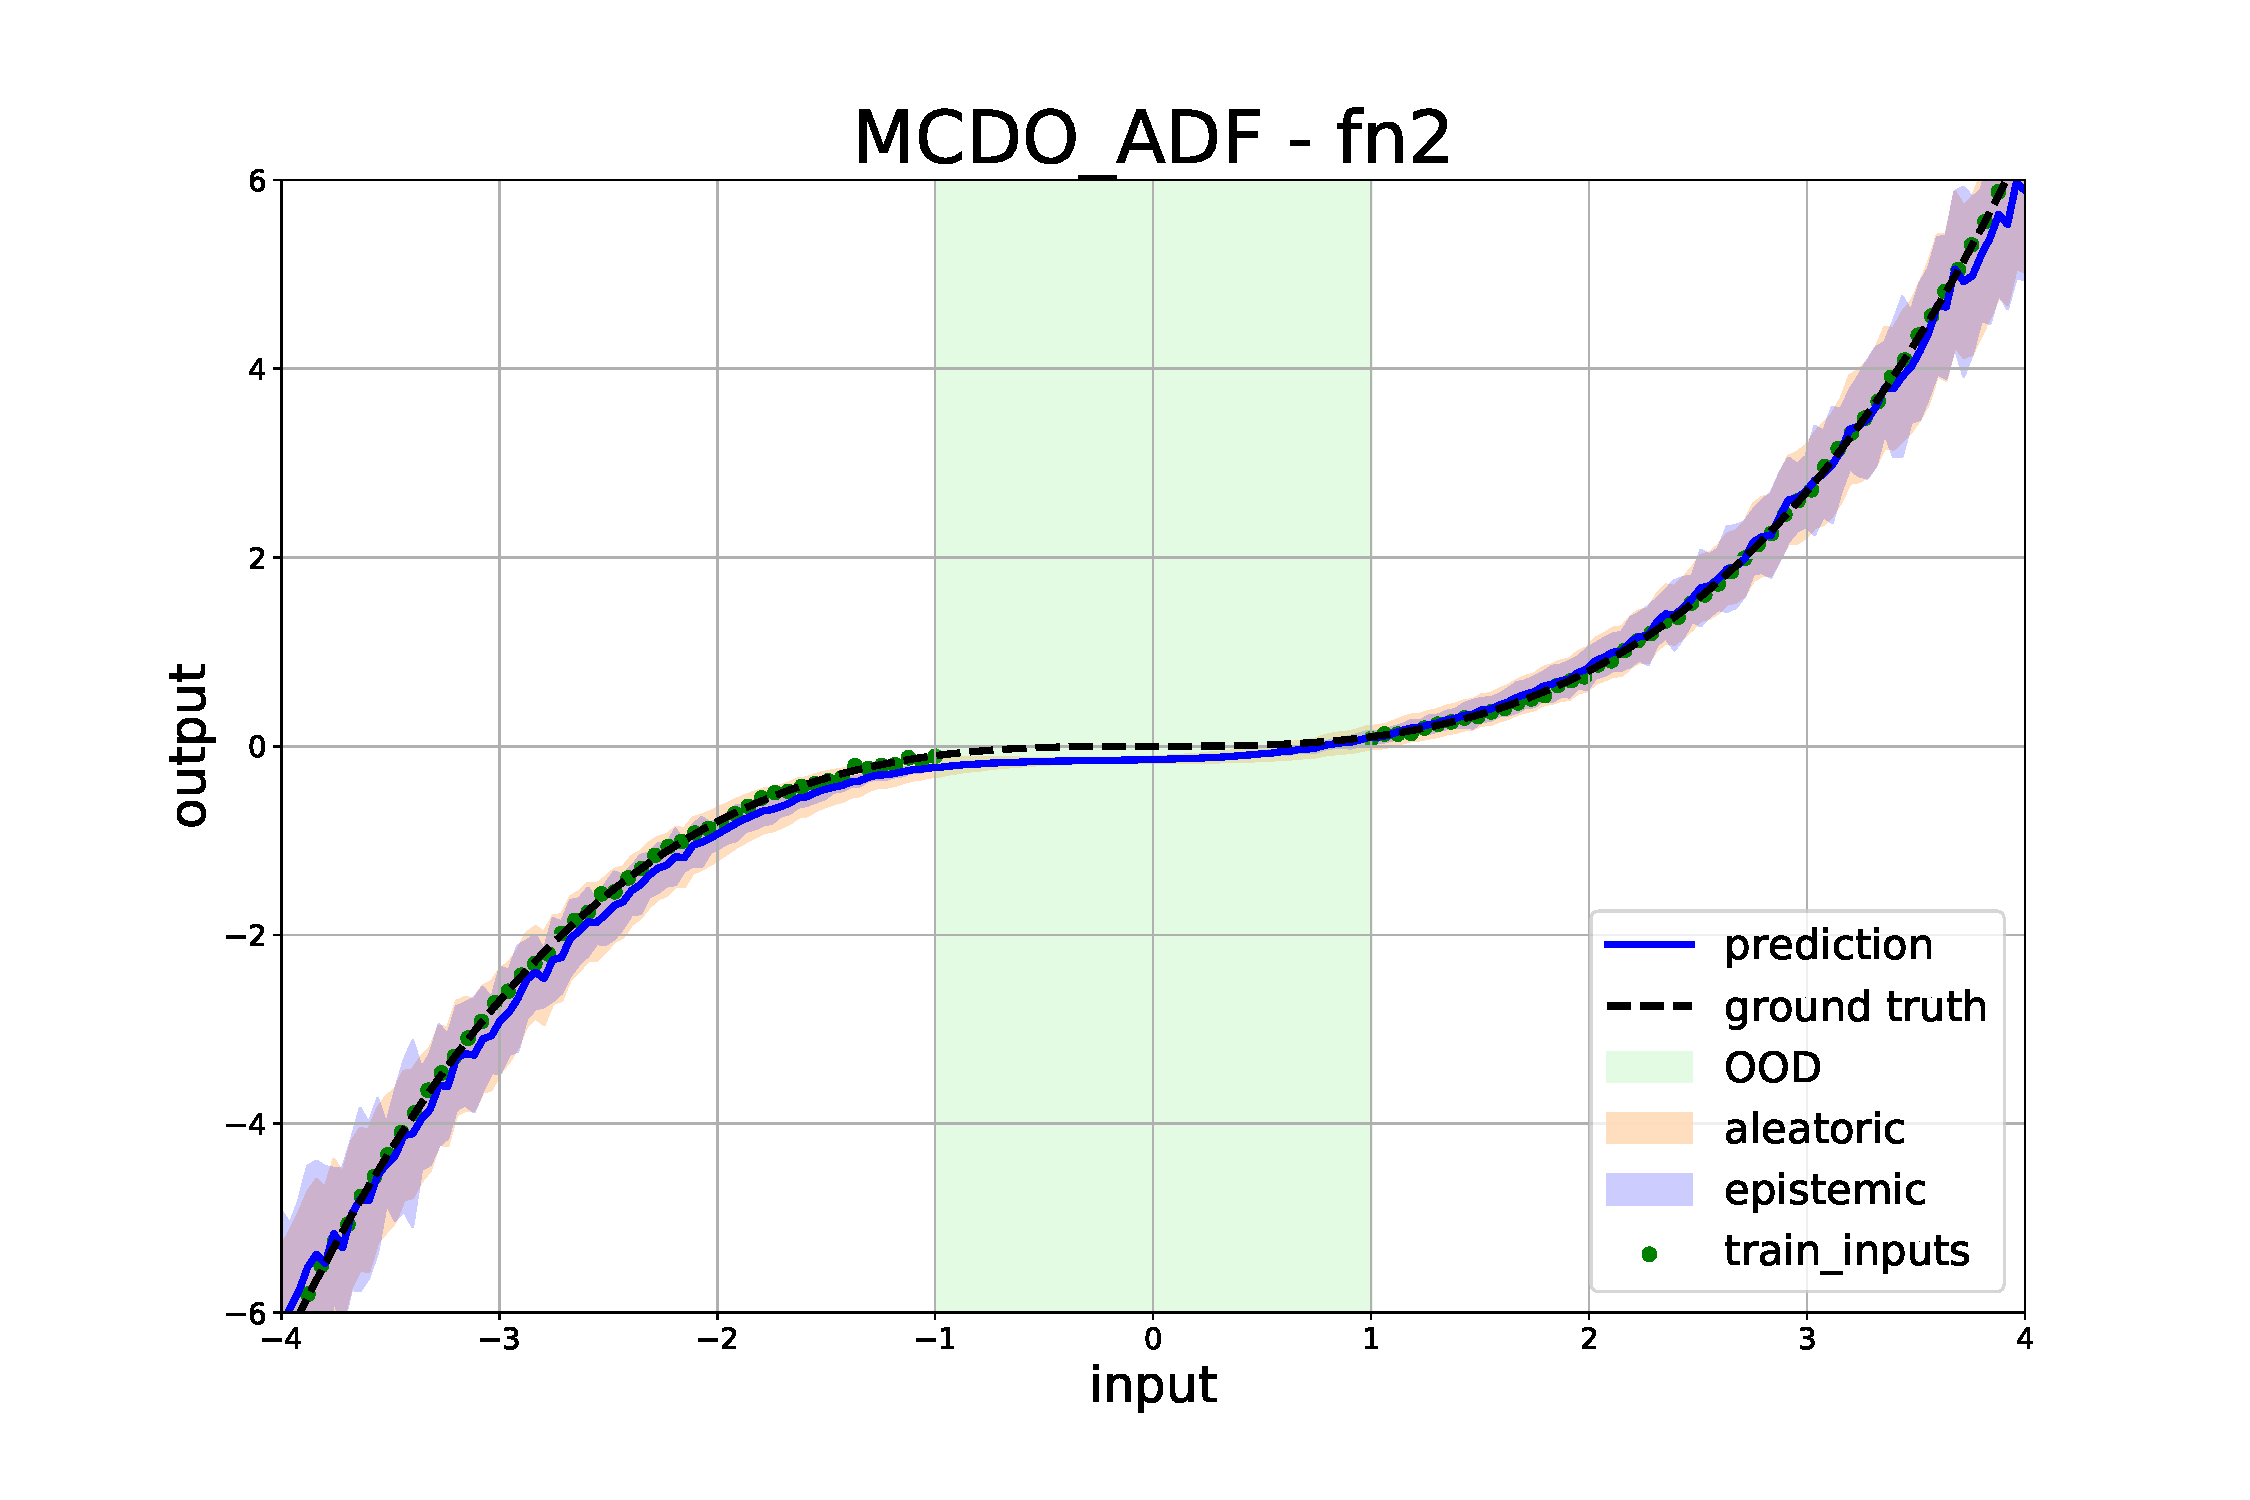
\includegraphics[width=\textwidth]{toy_dataset/mcdo_fn2}
		\caption{MCDO\_ADF on fn\_2: $y=0.1x^3$}
		\label{mcdo_fn2}
	\end{subfigure}
	\hfill
	\begin{subfigure}[b]{0.4\textwidth}
		\centering
		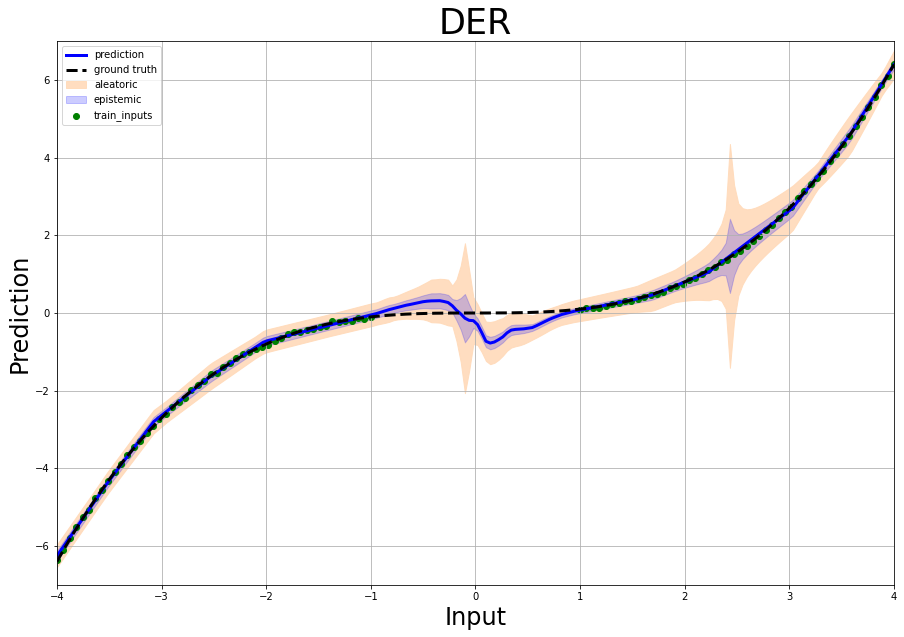
\includegraphics[width=\textwidth]{toy_dataset/der_fn2}
		\caption{DER on fn\_2: $y=0.1x^3$}
		\label{der_fn2}
	\end{subfigure}
	\hfill
	\begin{subfigure}[b]{0.4\textwidth}
		\centering
		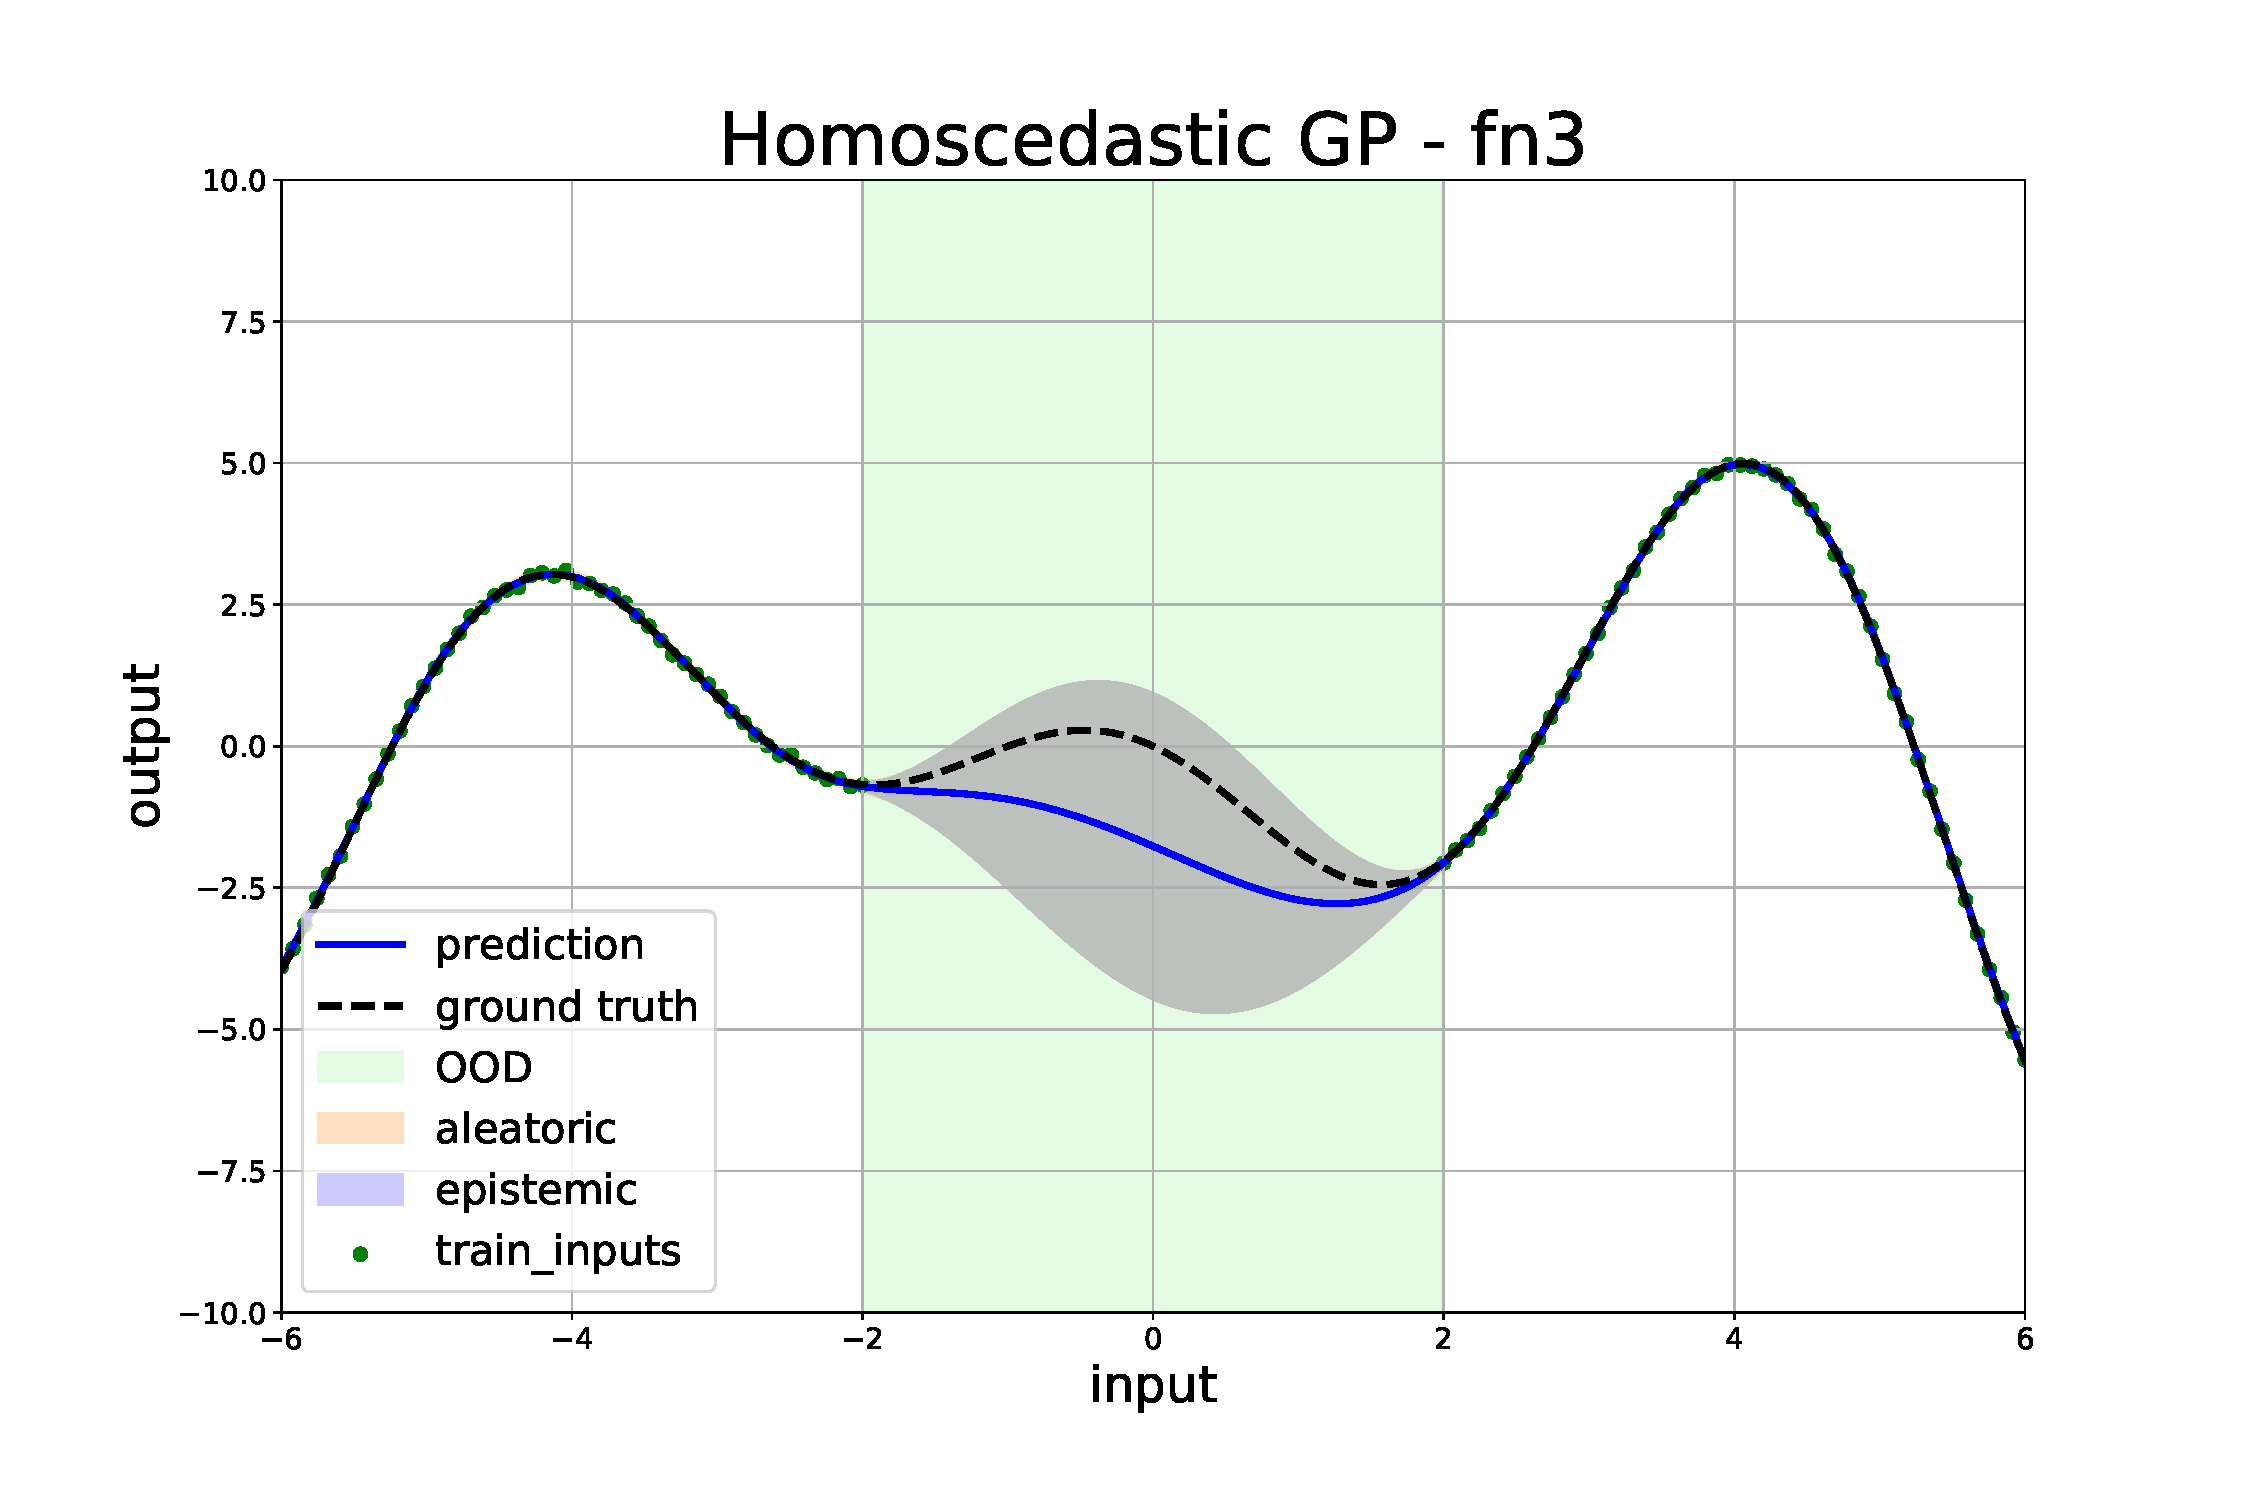
\includegraphics[width=\textwidth]{toy_dataset/homo_fn3}
		\caption{Homoscedastic GP on fn\_3: $y=-(1+x)sin(1.2x)$}
		\label{homo_fn3}
	\end{subfigure}
	\hfill
	\begin{subfigure}[b]{0.4\textwidth}
		\centering
		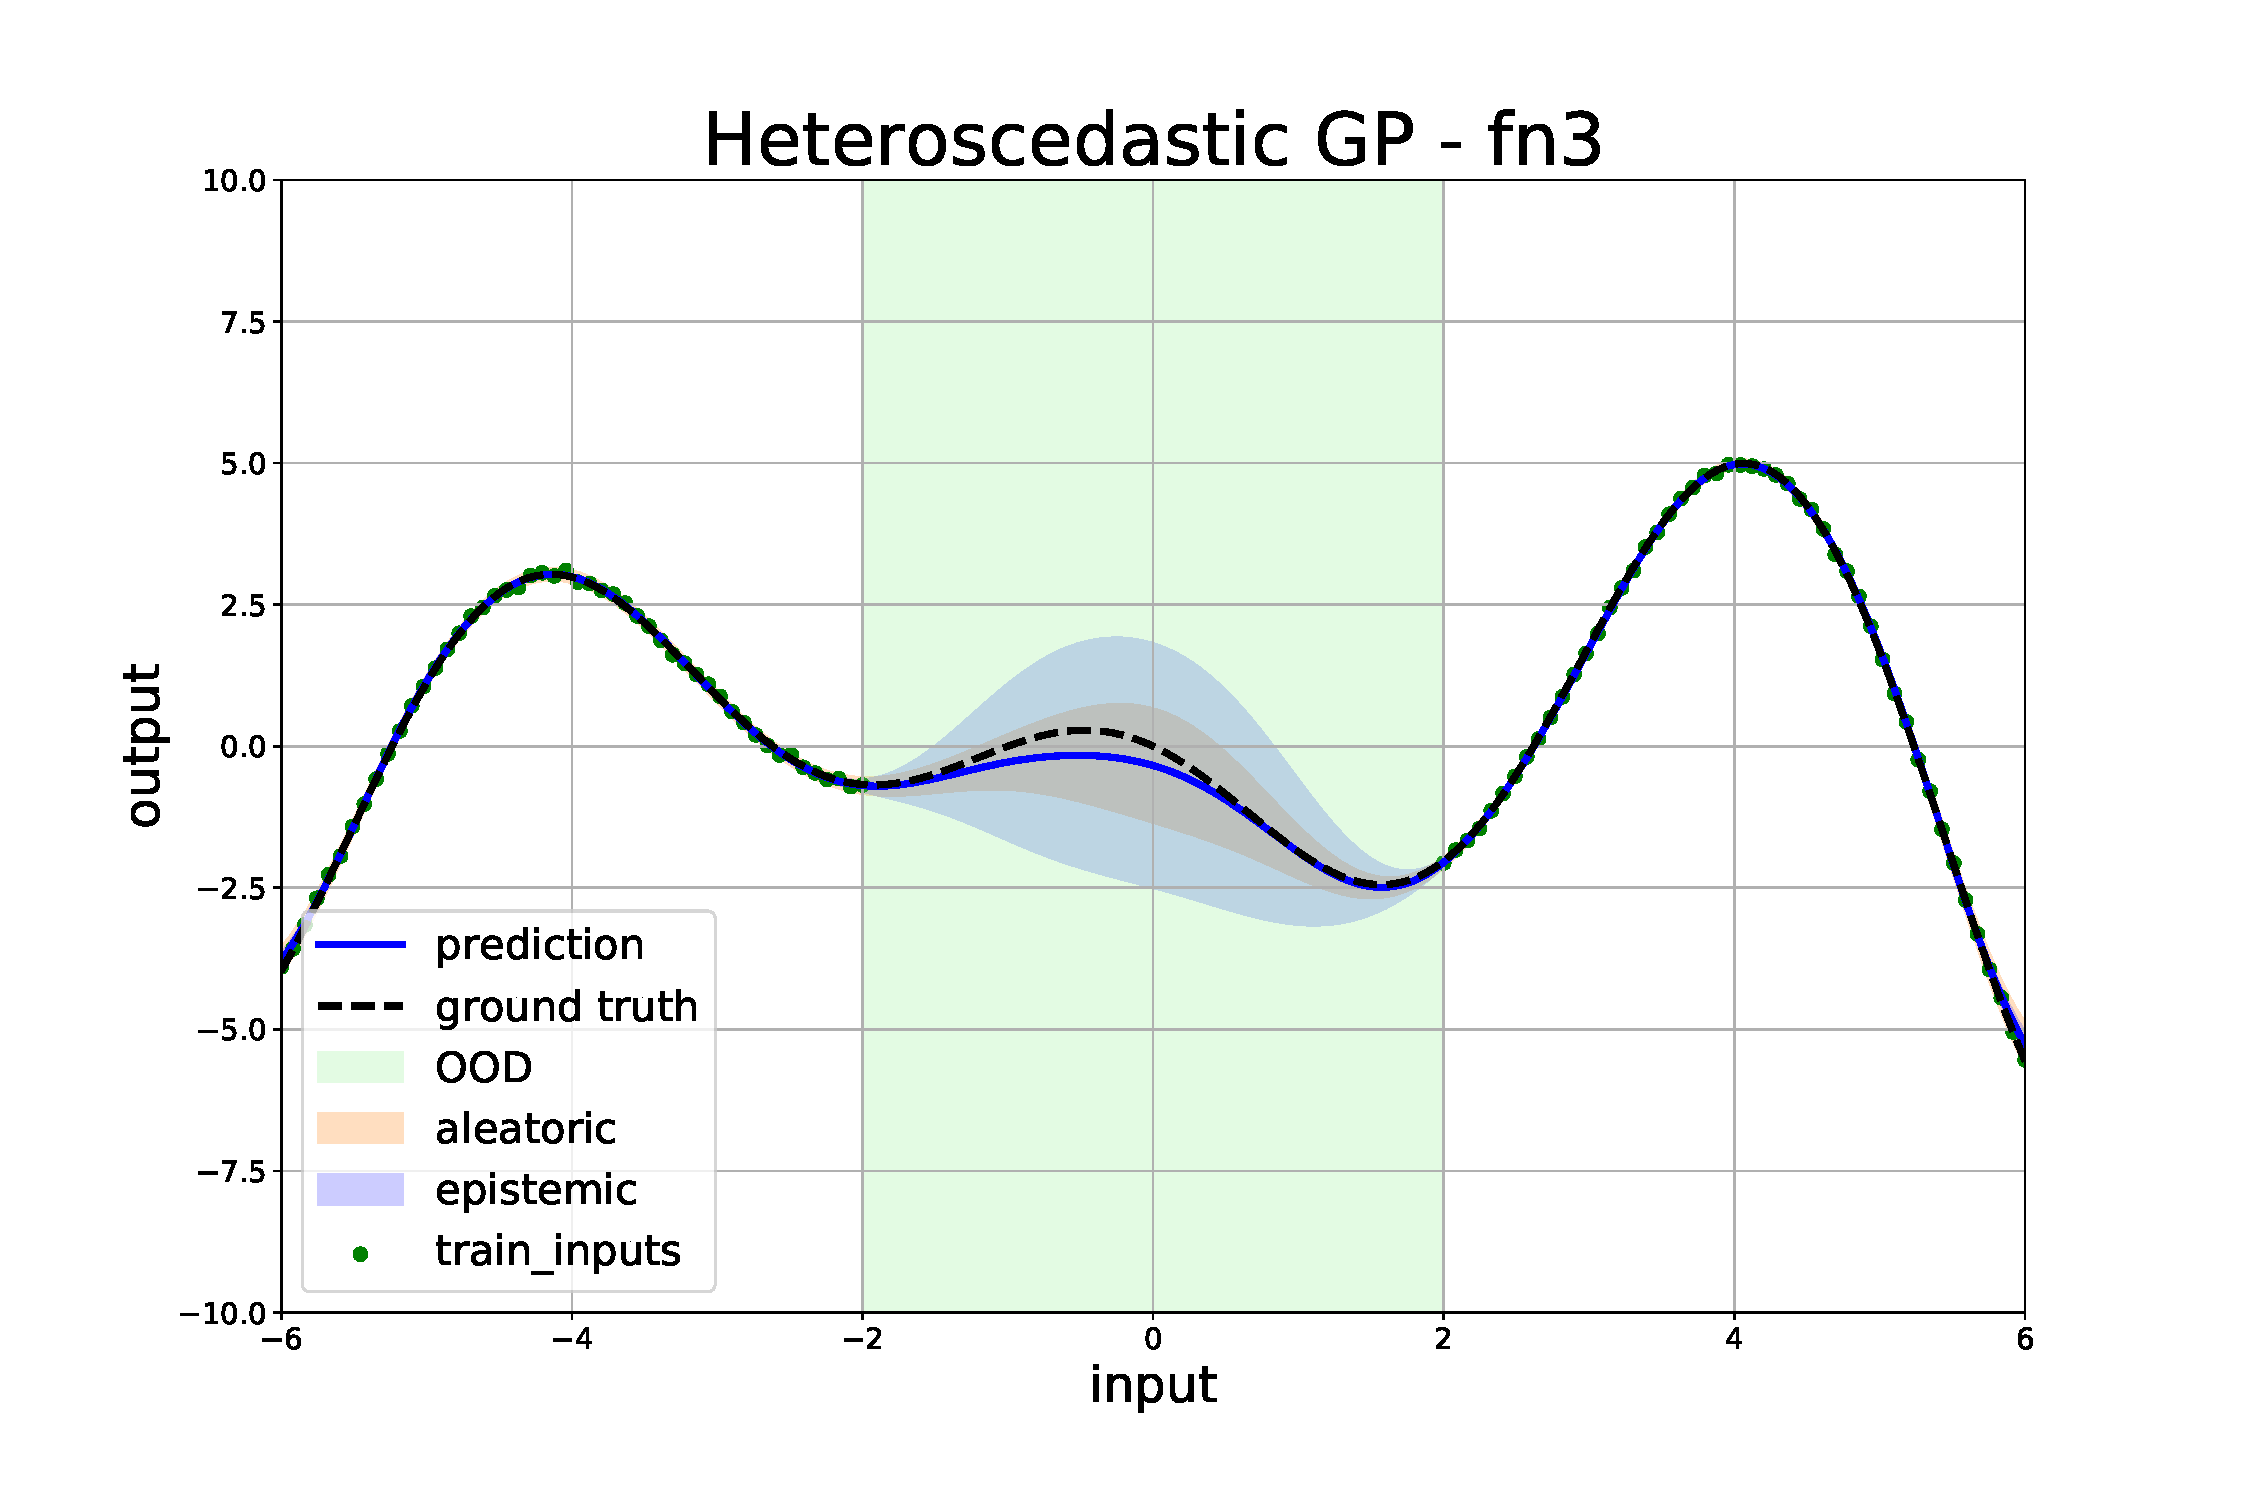
\includegraphics[width=\textwidth]{toy_dataset/hetero_fn3}
		\caption{Heteroscedastic GP on fn\_3: $y=-(1+x)sin(1.2x)$}
		\label{hetero_fn3}
	\end{subfigure}
	\hfill
	\begin{subfigure}[b]{0.4\textwidth}
		\centering
		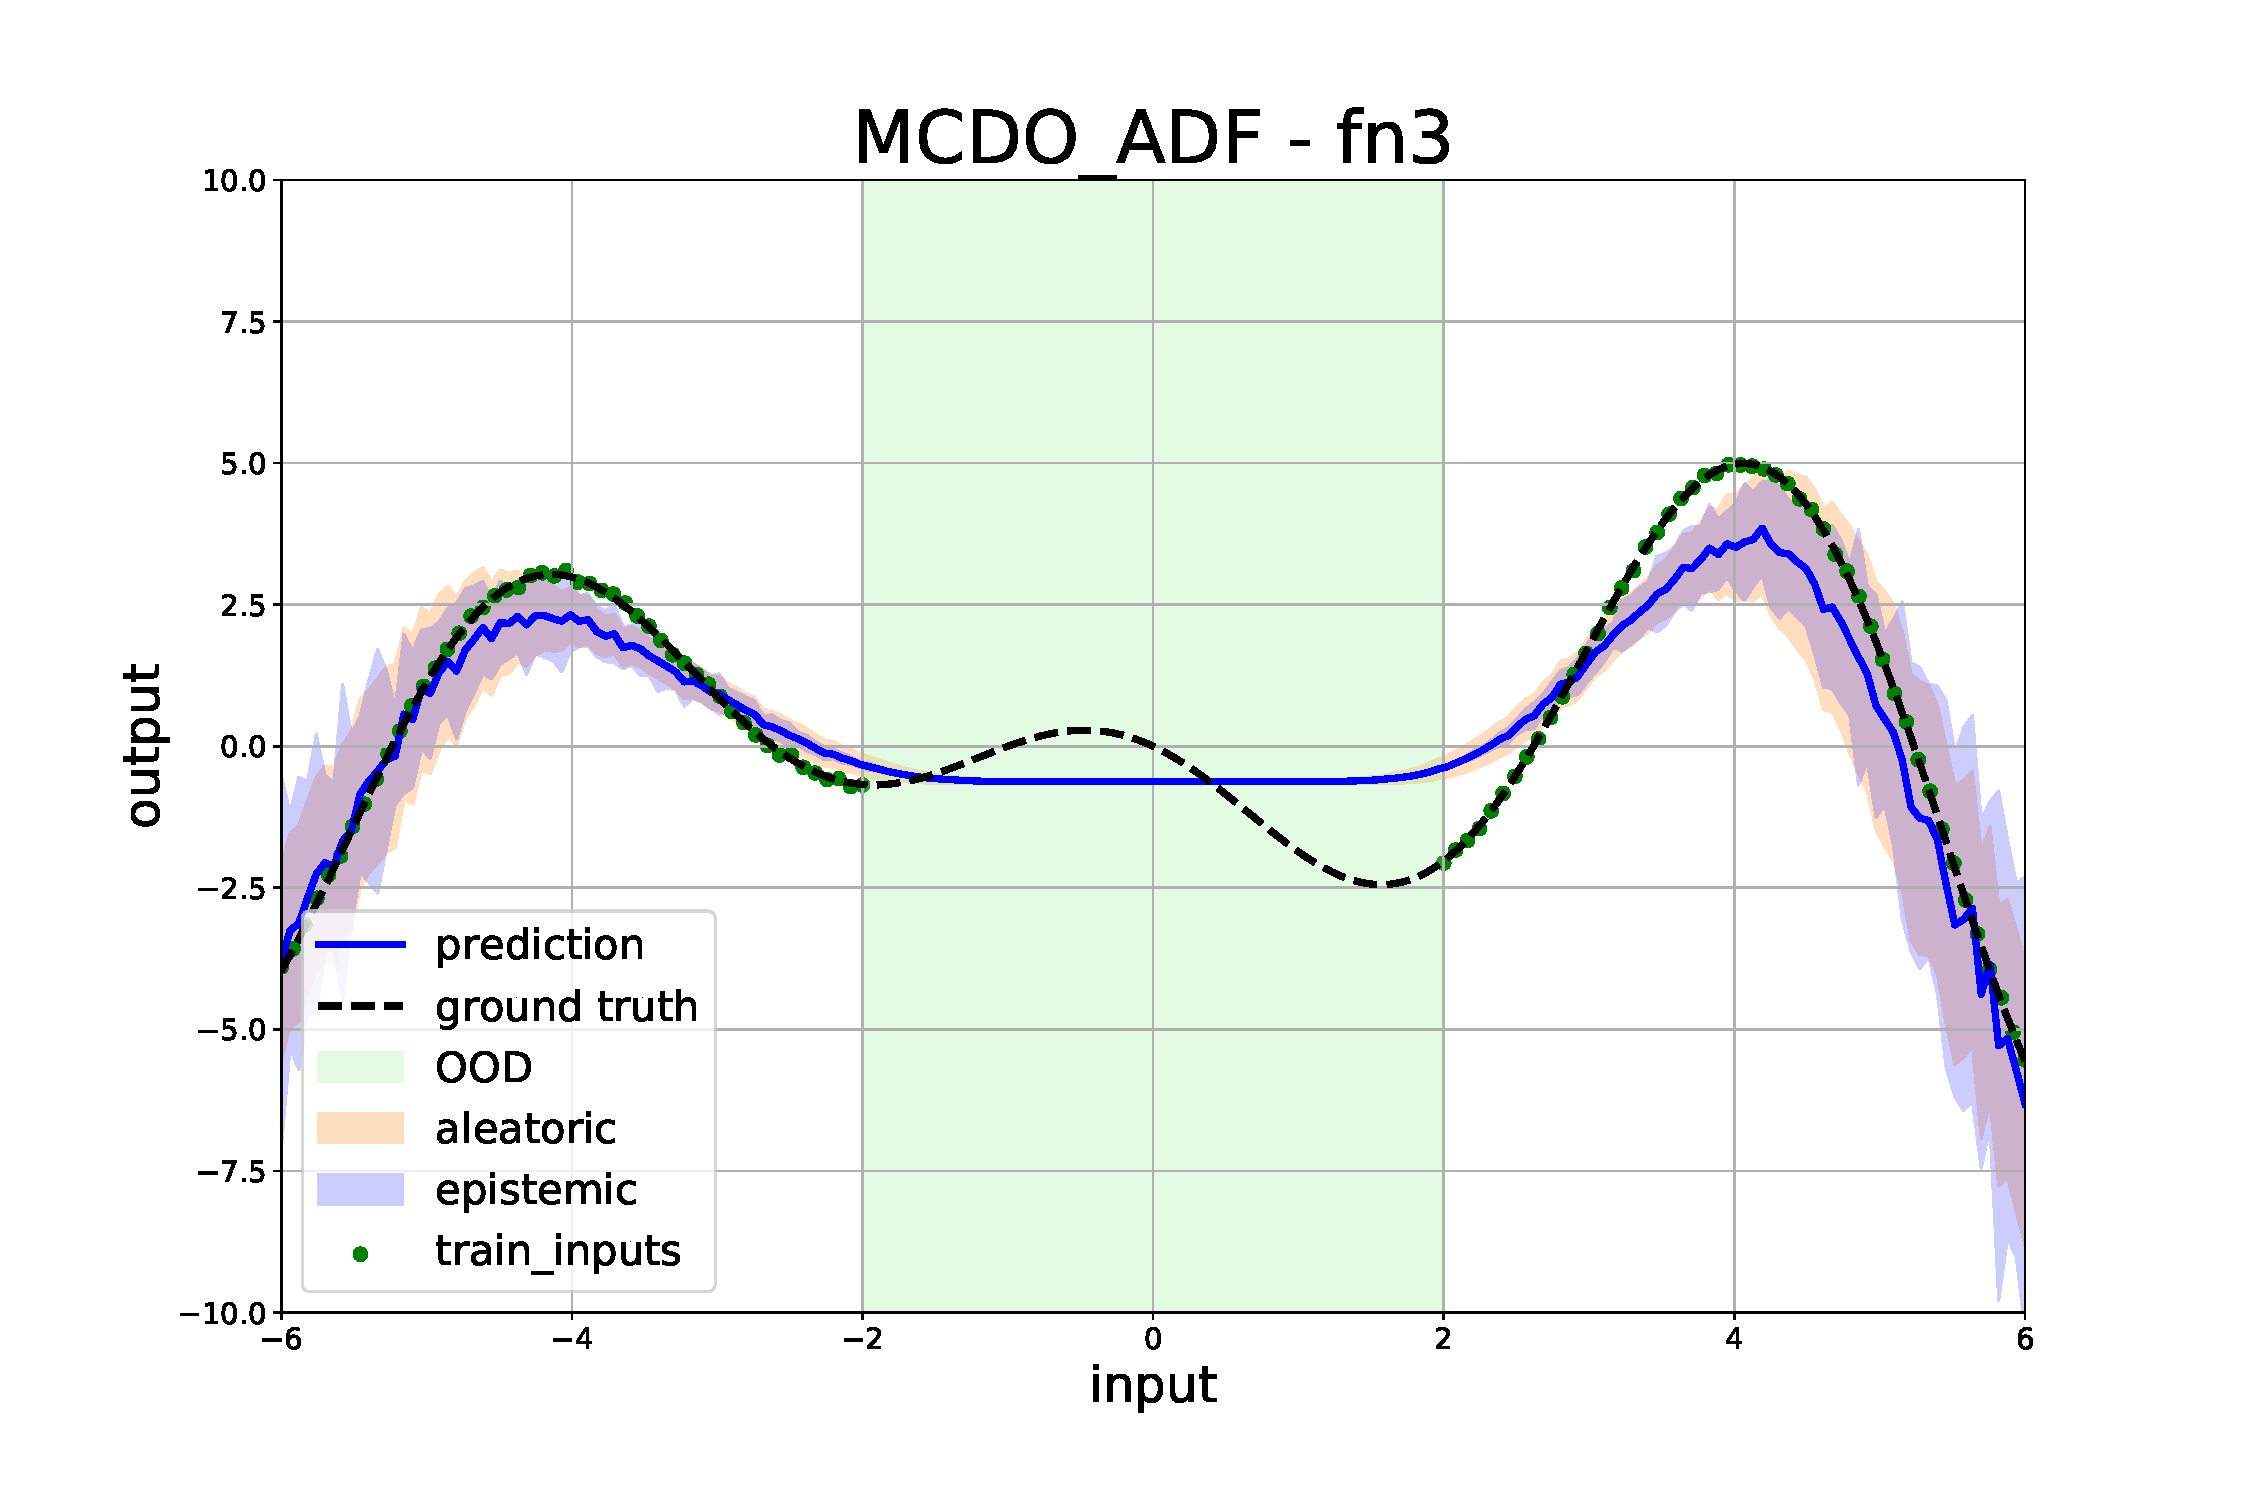
\includegraphics[width=\textwidth]{toy_dataset/mcdo_fn3}
		\caption{MCDO\_ADF on fn\_3: $y=-(1+x)sin(1.2x)$}
		\label{mcdo_fn3}
	\end{subfigure}
	\hfill
	\begin{subfigure}[b]{0.4\textwidth}
		\centering
		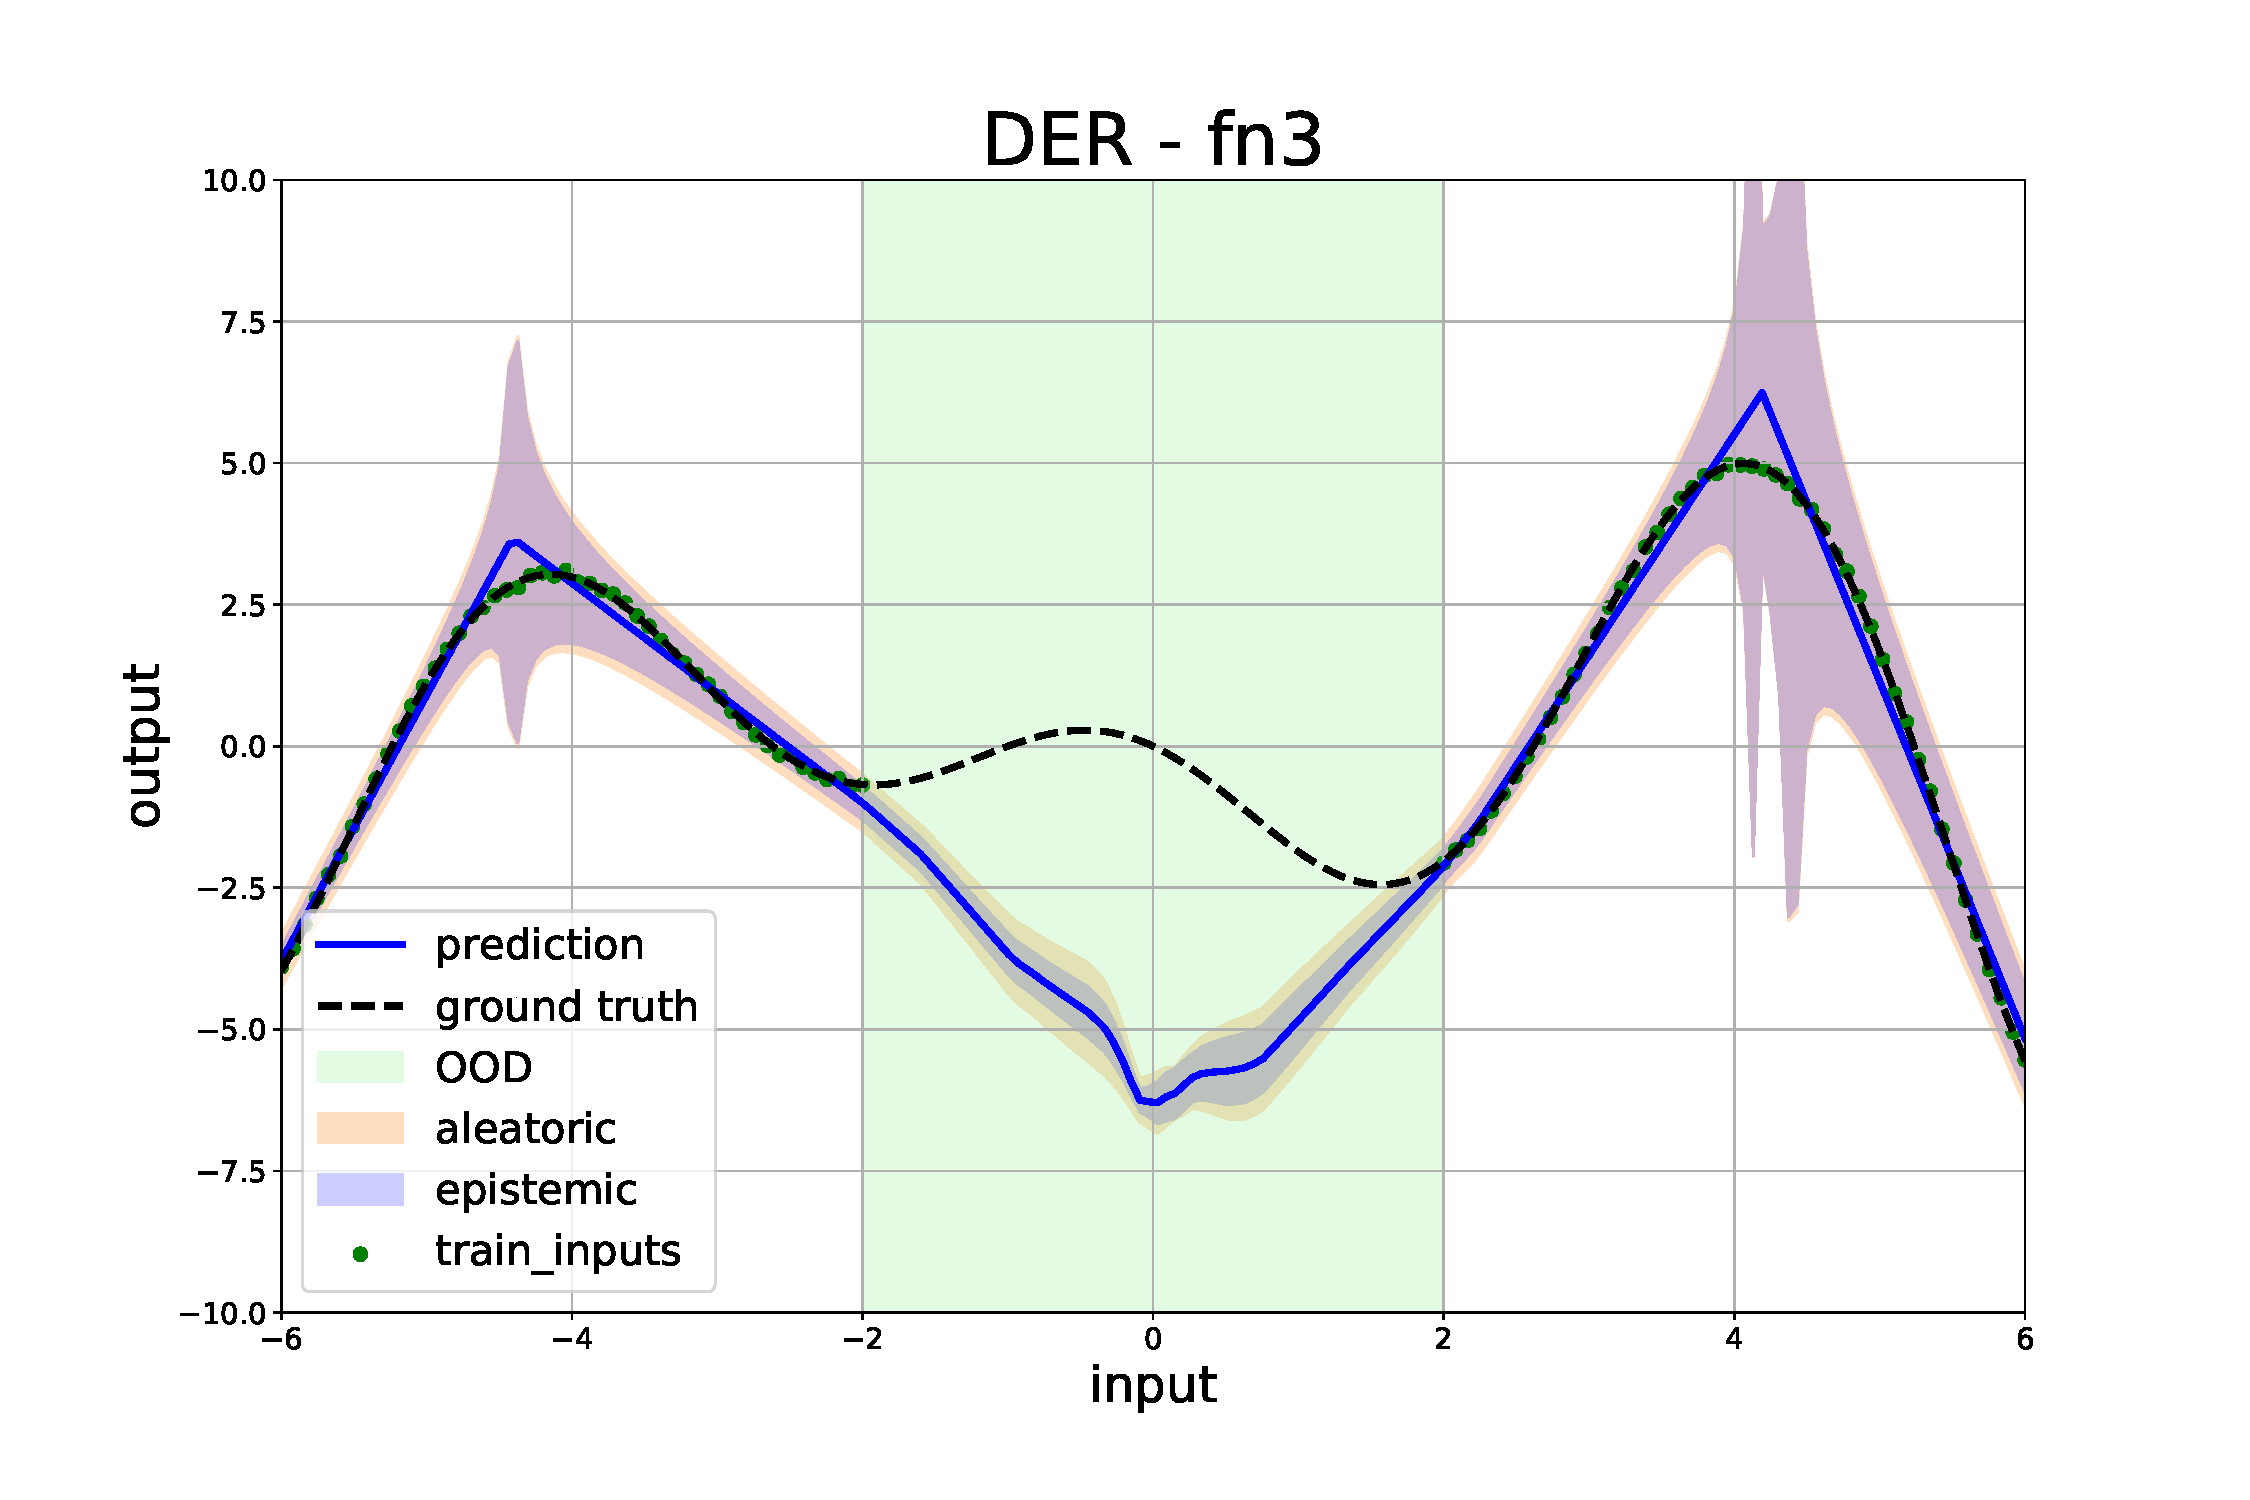
\includegraphics[width=\textwidth]{toy_dataset/der_fn3}
		\caption{DER on fn\_3: $y=-(1+x)sin(1.2x)$}
		\label{der_fn3}
	\end{subfigure}
	\hfill
	\caption{Plots depicting application of uncertainty estimation methods on 1D datasets}
	\label{fig_1d_functions}
\end{figure}


\vfill\section{Out-Of-Distribution(OOD) testing}
\subsubsection{\textbf{RQ3.} How do the identified uncertainty estimation methods compare with each other based on their response to Out-Of-Distribution(OOD) and adversarially perturbed inputs?}
One of the important uses for having an estimate of uncertainty associated with a Neural Net model's output is \enquote{selective prediction}. This means that the confidence estimate can be used to determine the correctness of an output and in turn decide whether to consider it for further processing/decision-making or not. It is crucial for the uncertainty estimation method to produce a higher value of uncertainty when the model faces test samples from an unknown data distribution. This section evaluates the considered uncertainty estimation methods on their response to out-of-distribution inputs.
\subsection {Response to Out-Of-Distribution data}\label{subsec_ood}
\subsubsection{Steering angle dataset}
In the qualitative comparison(\ref{sec_qual_comparison}) of methods on the steering angle data set, the relationship between uncertainty estimates and factors such as presence of blur, glare, sun-flare and illumination was discussed. In this section, the speculated relationship is validated. 
\begin{figure}[H]
	\centering
	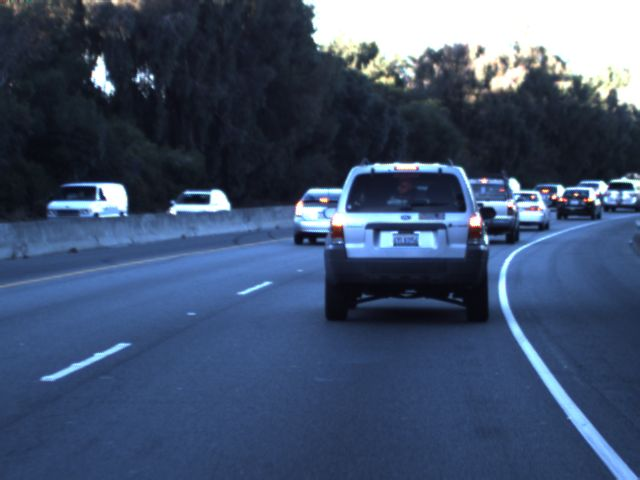
\includegraphics[width=0.4\textwidth]{noise/original}
	\caption{Image considered for OOD analysis}
	\label{fig_original_noise}
	\hfill
\end{figure}
\begin{figure}[H]
	\centering
	\begin{subfigure}[b]{0.18\textwidth}
		\centering
		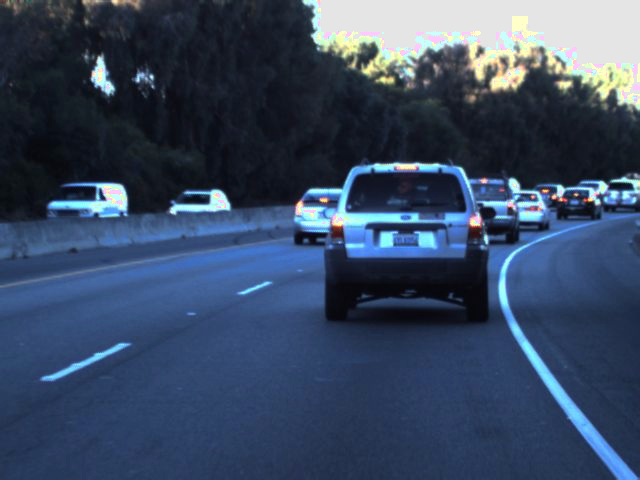
\includegraphics[width=\textwidth]{noise/dark_0}
		\caption{darkness\_coeff = 0.1}
		\label{mcdo_fn2}
	\end{subfigure}
	\hfill
	\begin{subfigure}[b]{0.18\textwidth}
		\centering
		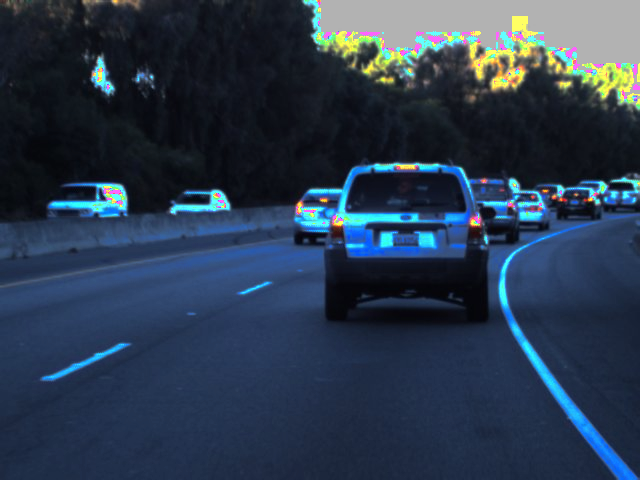
\includegraphics[width=\textwidth]{noise/dark_2}
		\caption{darkness\_coeff = 0.3}
		\label{der_fn2}
	\end{subfigure}
	\hfill
	\begin{subfigure}[b]{0.18\textwidth}
		\centering
		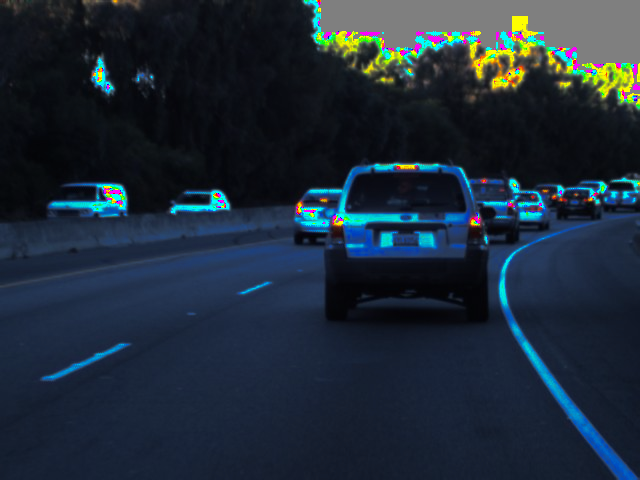
\includegraphics[width=\textwidth]{noise/dark_4}
		\caption{darkness\_coeff = 0.5}
		\label{homo_fn3}
	\end{subfigure}
	\hfill
	\begin{subfigure}[b]{0.18\textwidth}
		\centering
		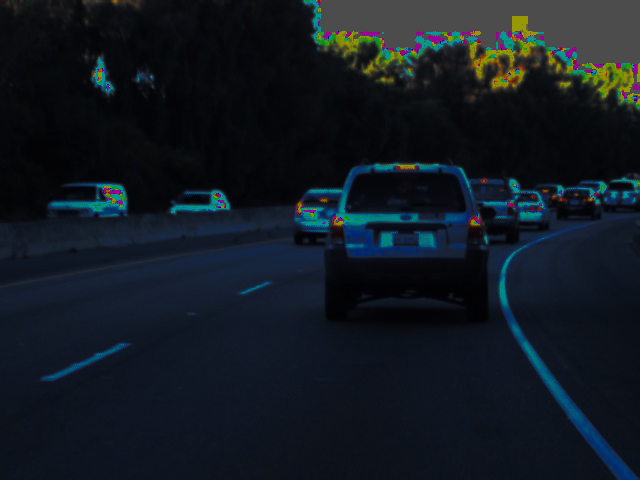
\includegraphics[width=\textwidth]{noise/dark_6}
		\caption{darkness\_coeff = 0.7}
		\label{hetero_fn3}
	\end{subfigure}
	\hfill
	\begin{subfigure}[b]{0.18\textwidth}
		\centering
		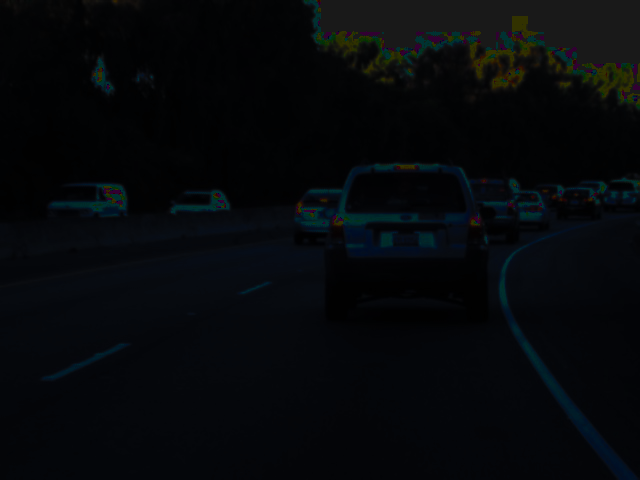
\includegraphics[width=\textwidth]{noise/dark_8}
		\caption{darkness\_coeff = 0.9}
		\label{mcdo_fn3}
	\end{subfigure}
	\hfill
	\label{fig_noise_dark}
\end{figure}
\begin{figure}[H]\ContinuedFloat
	\centering
	\begin{subfigure}[b]{0.18\textwidth}
		\centering
		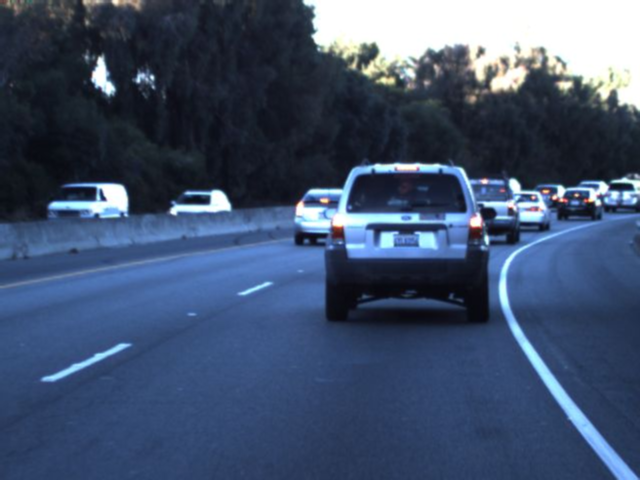
\includegraphics[width=\textwidth]{noise/fog_0}
		\caption{fog\_coeff = 0.1}
		\label{mcdo_fn2}
	\end{subfigure}
	\hfill
	\begin{subfigure}[b]{0.18\textwidth}
		\centering
		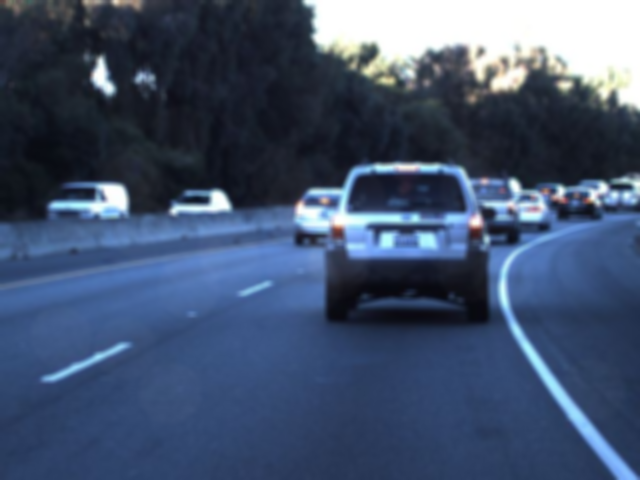
\includegraphics[width=\textwidth]{noise/fog_2}
		\caption{fog\_coeff = 0.3}
		\label{der_fn2}
	\end{subfigure}
	\hfill
	\begin{subfigure}[b]{0.18\textwidth}
		\centering
		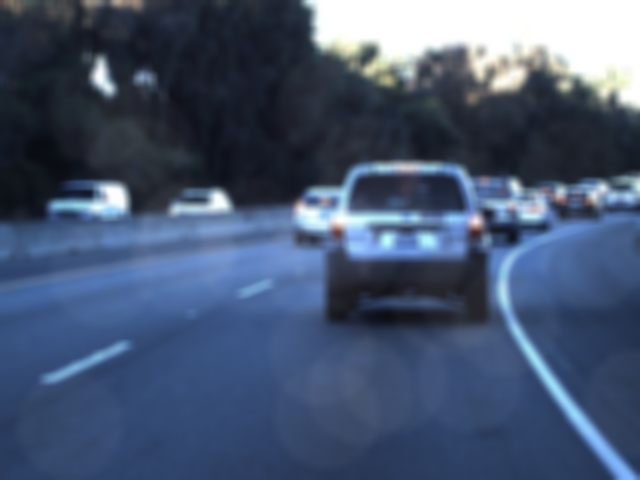
\includegraphics[width=\textwidth]{noise/fog_4}
		\caption{fog\_coeff = 0.5}
		\label{homo_fn3}
	\end{subfigure}
	\hfill
	\begin{subfigure}[b]{0.18\textwidth}
		\centering
		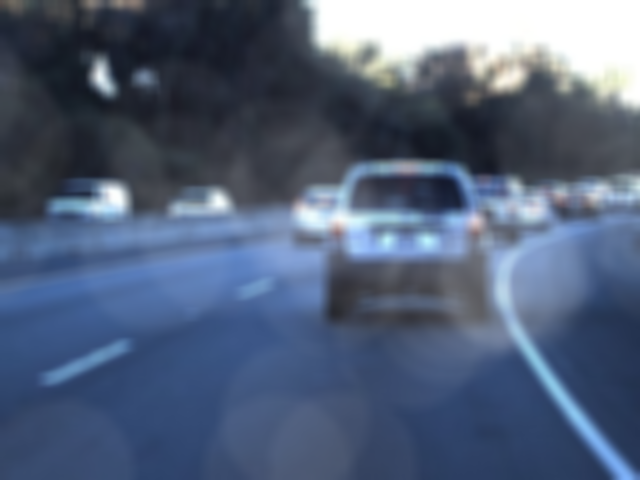
\includegraphics[width=\textwidth]{noise/fog_6}
		\caption{fog\_coeff = 0.7}
		\label{hetero_fn3}
	\end{subfigure}
	\hfill
	\begin{subfigure}[b]{0.18\textwidth}
		\centering
		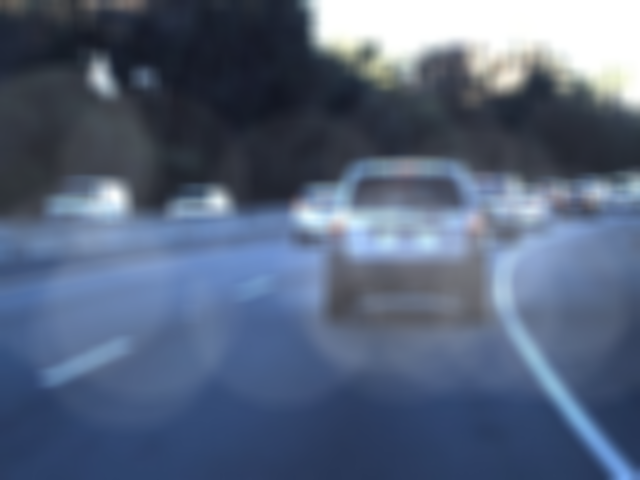
\includegraphics[width=\textwidth]{noise/fog_8}
		\caption{fog\_coeff = 0.9}
		\label{mcdo_fn3}
	\end{subfigure}
	\hfill
	%\caption{A subset of synthesized images introducing increasing levels of fog}
	\label{fig_noise_fog}
\end{figure}
\begin{figure}[H]\ContinuedFloat
	\centering
	\begin{subfigure}[b]{0.18\textwidth}
		\centering
		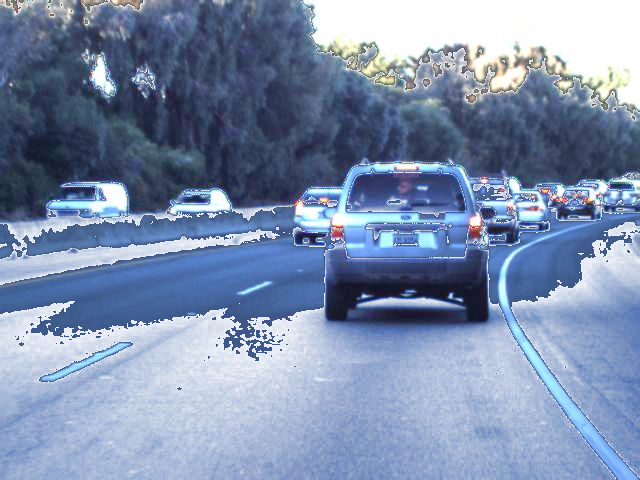
\includegraphics[width=\textwidth]{noise/snow_0}
		\caption{snow\_coeff = 0.1}
		\label{mcdo_fn2}
	\end{subfigure}
	\hfill
	\begin{subfigure}[b]{0.18\textwidth}
		\centering
		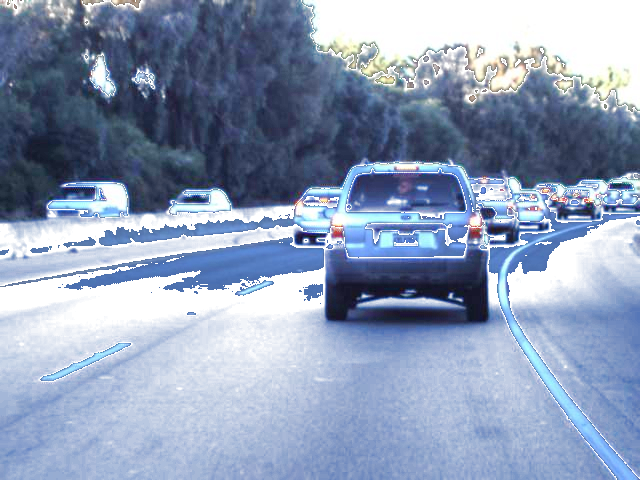
\includegraphics[width=\textwidth]{noise/snow_2}
		\caption{snow\_coeff = 0.3}
		\label{der_fn2}
	\end{subfigure}
	\hfill
	\begin{subfigure}[b]{0.17\textwidth}
		\centering
		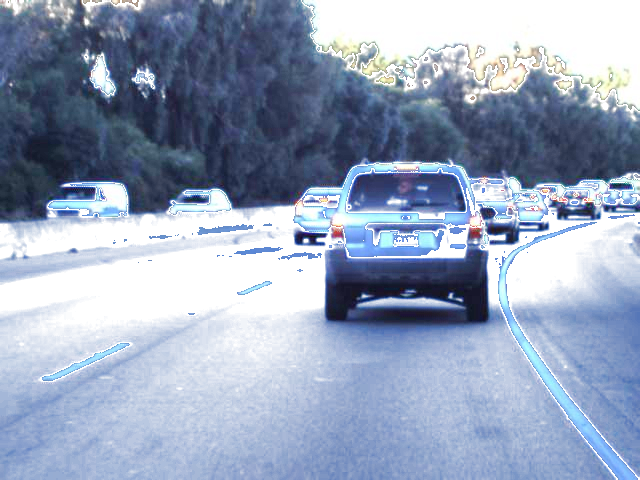
\includegraphics[width=\textwidth]{noise/snow_4}
		\caption{snow\_coeff = 0.5}
		\label{homo_fn3}
	\end{subfigure}
	\hfill
	\begin{subfigure}[b]{0.18\textwidth}
		\centering
		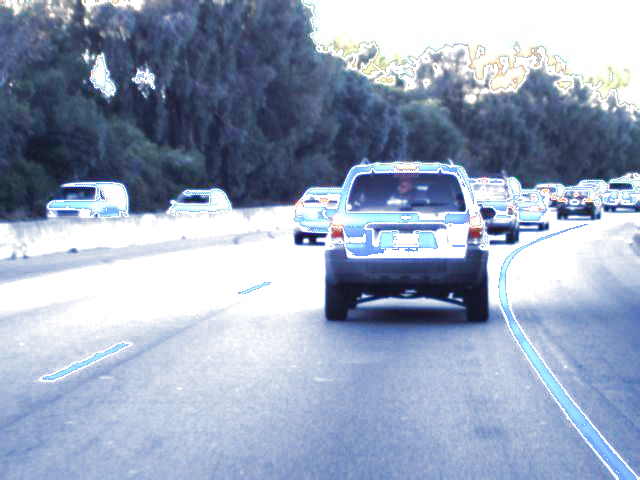
\includegraphics[width=\textwidth]{noise/snow_6}
		\caption{snow\_coeff = 0.7}
		\label{hetero_fn3}
	\end{subfigure}
	\hfill
	\begin{subfigure}[b]{0.18\textwidth}
		\centering
		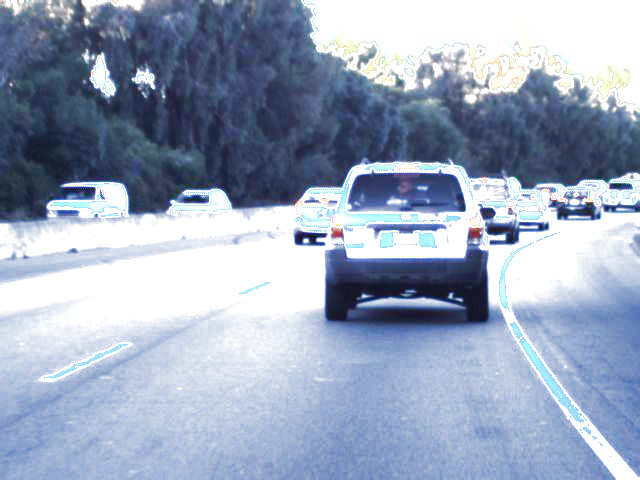
\includegraphics[width=\textwidth]{noise/snow_8}
		\caption{snow\_coeff = 0.9}
		\label{mcdo_fn3}
	\end{subfigure}
	\hfill
	\caption{A subset of synthesized images introducing increasing levels of darkness, fog and snow}
	\label{fig_noise_fog}
\end{figure}
Using image processing techniques, three sets of images are generated by introducing fog, snow-like patterns, and darkness to a noise-less image(\ref{fig_original_noise}) chosen from the steering angle dataset. These images are fed as inputs to both MCDO\_ADF and DER model variants and  responses of their respective uncertainty estimation methods are evaluated.
\subsubsection{Analysis}
\begin{itemize}
	\item Darkness: Increasing levels of darkness almost does not have any impact on total uncertainty estimated by DER. While an increase in uncertainty estimates of MCDO\_ADF can be observed for initial levels of darkness the trend do not remain for higher values which makes the method's response undesirable. When it comes to predictive error, absolute deviation values of the DER model variant is better aligned with increasing levels of darkness than its MCDO\_ADF counterpart. 
	\item Fog: Though exist few inconsistencies, MCDO\_ADF's estimates of total uncertainty are better aligned with increasing levels of fog than DER. The same holds true for the relationship between fog levels and predictive error as well.
	\item Snow: While DER's response in terms of uncertainty estimates remains almost constant to changes in levels of snow, a peculiar trend can be observed in MCDO\_ADF's output that the values of uncertainty decrease with increase in snow levels. There does not exist a strong correlation between the levels of snow and predictive error values corresponding to both the model variants. 
\end{itemize}
Except for the case of images with different levels of fog where MCDO\_ADF shows a desirable response, any significant relationship between the considered set of variables could not be established, in the other two cases. Observations such as unchanging values of uncertainty estimated by DER for increasing levels of fog and snow and existence alignment between uncertainty estimates and predictive error of the DER model variant in the case of dark images, show that factors such as model calibration and invariance of a model to a feature have a role to play. In order to better understand responses of the chosen pair of uncertainty estimation methods to OOD inputs, the analysis is extended to the test split of the steering angle dataset.
\begin{figure}[H]
	\centering
	\begin{subfigure}[b]{0.4\textwidth}
		\centering
		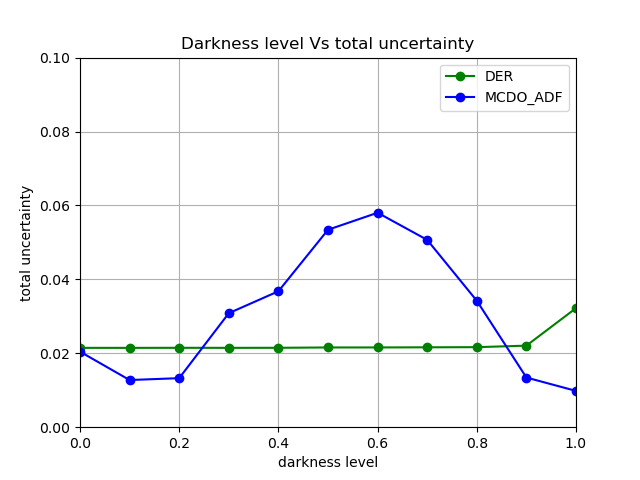
\includegraphics[width=\textwidth]{noise/dark-uncertainty}
		\caption{Levels of darkness Vs Total uncertainty}
		\label{mcdo_fn2}
	\end{subfigure}
	\hfill
	\begin{subfigure}[b]{0.4\textwidth}
		\centering
		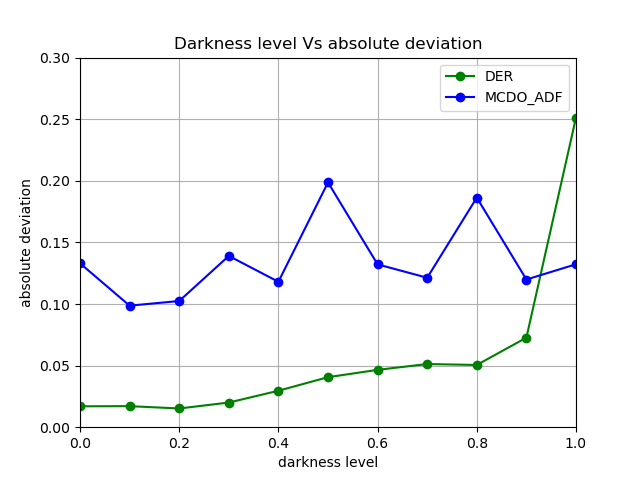
\includegraphics[width=\textwidth]{noise/dark-error}
		\caption{Levels of darkness Vs Absolute deviation}
		\label{der_fn2}
	\end{subfigure}
	\hfill
	\begin{subfigure}[b]{0.4\textwidth}
		\centering
		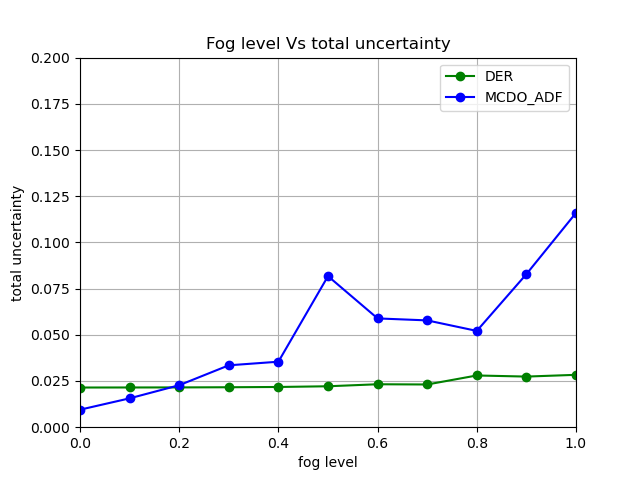
\includegraphics[width=\textwidth]{noise/fog-uncertainty}
		\caption{Levels of fog Vs Total uncertainty}
		\label{homo_fn3}
	\end{subfigure}
	\hfill
	\begin{subfigure}[b]{0.4\textwidth}
		\centering
		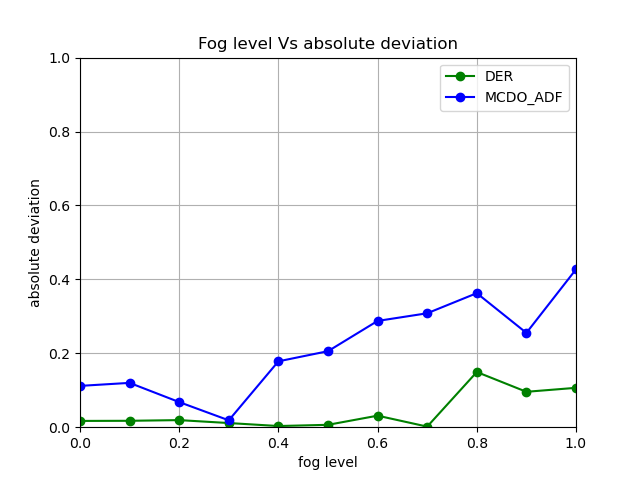
\includegraphics[width=\textwidth]{noise/fog-error}
		\caption{Levels of fog Vs Absolute deviation}
		\label{hetero_fn3}
	\end{subfigure}
	\hfill
	\begin{subfigure}[b]{0.4\textwidth}
		\centering
		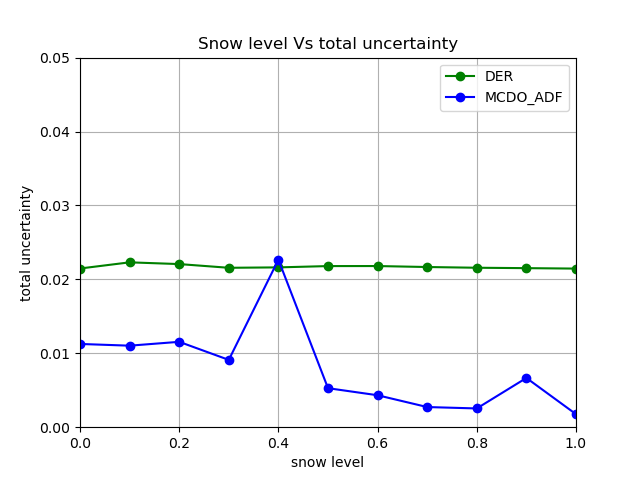
\includegraphics[width=\textwidth]{noise/snow-uncertainty}
		\caption{Levels of snow Vs Total uncertainty}
		\label{mcdo_fn3}
	\end{subfigure}
	\hfill
	\begin{subfigure}[b]{0.4\textwidth}
	\centering
	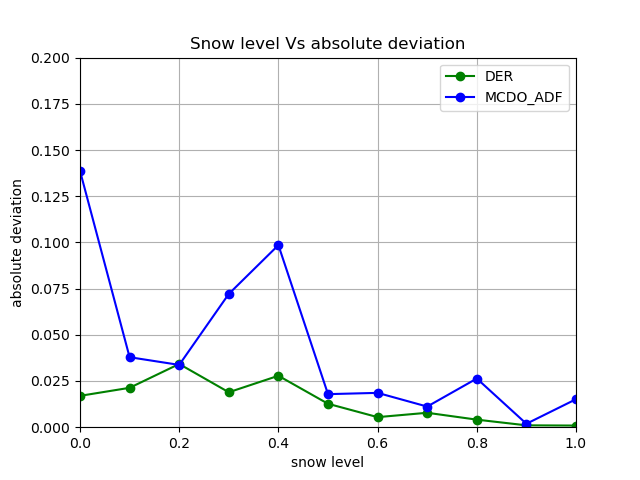
\includegraphics[width=\textwidth]{noise/snow-error}
	\caption{Levels of snow Vs Absolute deviation}
	\label{mcdo_fn3}
	\end{subfigure}
	\hfill
	\caption{Response to Out-Of-Distribution images (steering angle dataset)}
	\label{fig_noise_fog}
\end{figure}
\subsubsection{Extended analysis}\label{ood_extended}
Plots in the Figure \ref{fig_ood_extended} depict the change in values of uncertainties(averaged over all outputs) and RMSE with respect to increase in darkness level of input images. Existence of an almost linear relationship between increasing darkness level in images and prediction error (RMSE) values of both DER and MCDO\_ADF models is observed. This indicates that both the models are well-calibrated. The MCDO\_ADF method clearly outperforms DER in appropriateness of its response to increasing darkness levels in images, by producing high-valued uncertainty estimates. However its response is inconsistent as uncertainty values(epistemic, aleatoric and total) surge sharply as the darkness coefficient value exceeds 0.7. The reason for this sudden drop could not be determined. In the case of DER, uncertainty levels mostly remain constant and few fluctuations occur. Therefore, any significant relationship could not be established between darkness levels and corresponding uncertainty estimates produced by both the methods. 

\begin{figure}[H]
	\centering
	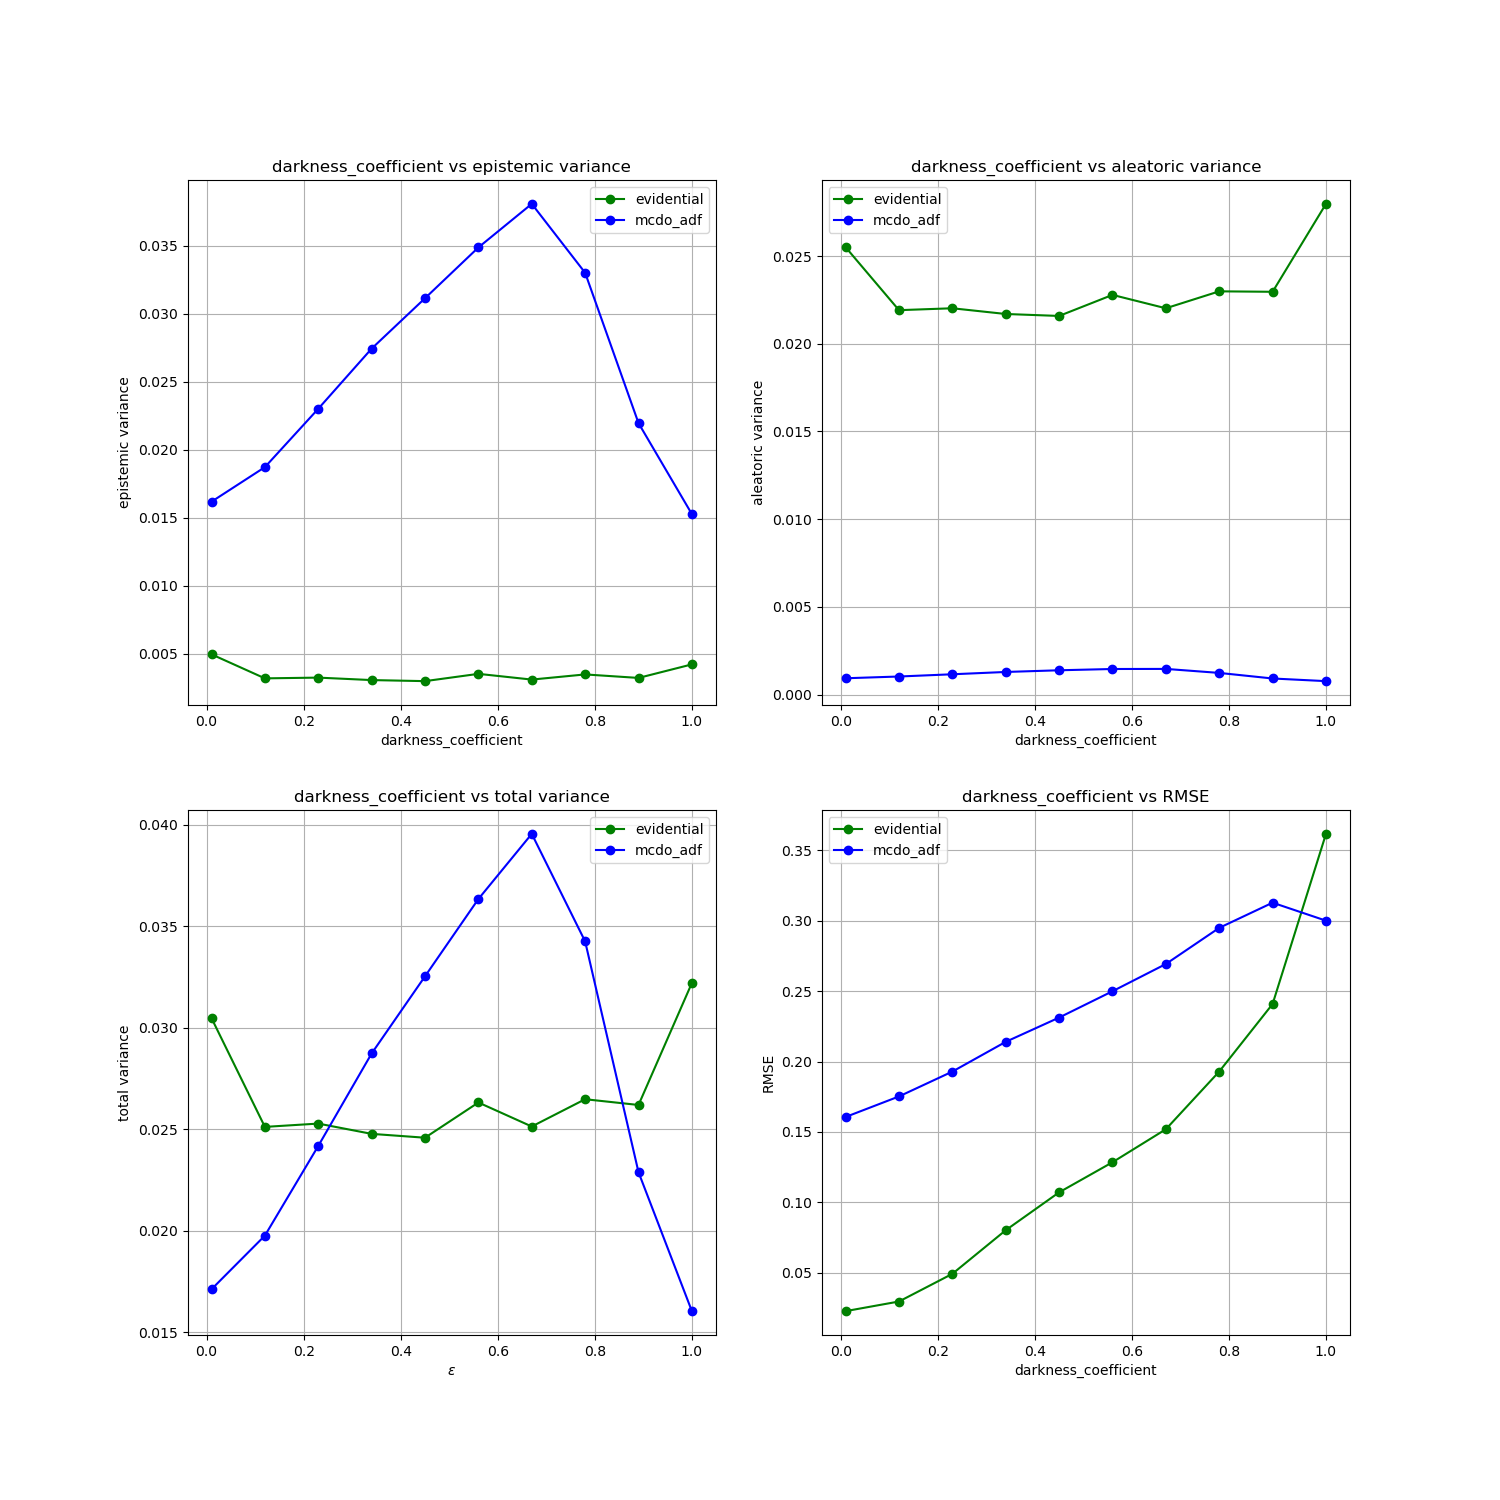
\includegraphics[scale=0.34]{ood/noise_plots}
	\caption{Response to Out-Of-Distribution images(extended analysis) }
	\label{fig_ood_extended}
	\hfill
\end{figure}
\subsubsection{1D datasets}
Train and test data ranges of the set of 1D functions are set in such a way that the Out-Of-Distribution (OOD) regions lie both in-between and on either sides of training data ranges. Owing to the smooth nature of target functions and use of squared exponential kernels GPs perform well both in terms of predictive accuracy and NLL(uncertainty estimation quality) in OOD areas. Both the considered uncertainty estimation methods do not perform well in predicting the mean and estimating uncertainties in OOD regions of fn\_3. Due to narrow confidence intervals proposed by MCDO\_ADF in this region, the method performs poorly in terms of NLL. In the case of fn\_2, predictions of both the methods remain close to the target. The MCDO\_ADF method outperforms DER by reporting a high value of epistemic uncertainty for OOD regions in fn\_1. 
\subsection{Response to adversarial attacks(for steering angle dataset only)}\label{subsec_adv}
\begin{figure}[H]
	\centering
	\begin{subfigure}[b]{0.19\textwidth}
		\centering
		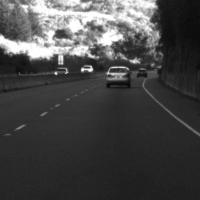
\includegraphics[width=\textwidth]{adv_0}
		\caption{$\epsilon=0$}
		\label{fig:y equals x}
	\end{subfigure}
	\hfill
	\begin{subfigure}[b]{0.19\textwidth}
		\centering
		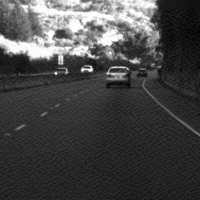
\includegraphics[width=\textwidth]{adv_1}
		\caption{$\epsilon=0.02$}
		\label{fig:three sin x}
	\end{subfigure}
	\hfill
	\begin{subfigure}[b]{0.19\textwidth}
		\centering
		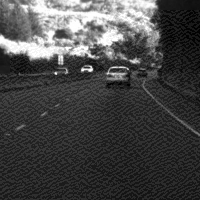
\includegraphics[width=\textwidth]{adv_2}
		\caption{$\epsilon=0.06$}
		\label{fig:five over x}
	\end{subfigure}
	\hfill
	\begin{subfigure}[b]{0.19\textwidth}
		\centering
		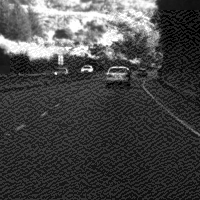
\includegraphics[width=\textwidth]{adv_3}
		\caption{$\epsilon=0.08$}
		\label{fig:five over x}
	\end{subfigure}
	\hfill
	\begin{subfigure}[b]{0.19\textwidth}
		\centering
		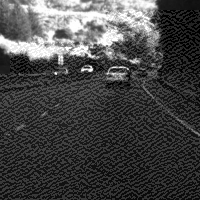
\includegraphics[width=\textwidth]{adv_4}
		\caption{$\epsilon=0.10$}
		\label{fig:five over x}
	\end{subfigure}
	\caption{Increasing levels of adversarial noise}
	\label{fig_adv_example}
\end{figure}

Adversarial examples are malicious inputs designed to fool machine learning models[\cite{kurakin2016adversarial}]. Such data samples can be considered as an extreme case of Out-Of-Distribution as they are synthesized by perturbing inputs in an adversarial fashion to cause maximum error on the model prediction. An uncertainty estimation method needs to be capable of identifying and reporting an adversarially perturbed input data sample by producing a high value of uncertainty. 
In order to evaluate responses of the considered uncertainty estimation methods, samples from training data distribution are perturbed using the FGSM(Fast Gradient Sign Method)\cite{goodfellow2015explaining} and fed to models. A set of images produced from a given image subject to different levels of adversarial perturbations is shown in the Figure\ref{fig_adv_example}. Adversarial images fed to a given Dronet model variant are synthesized using perturbations generated by its own.  
Plots in the Figure \ref{fig_adv_analysis} depict the impact of increasing perturbation levels(denoted by $\epsilon$) on average values of uncertainty estimates and RMSE values respectively, for both model variants. The following can be inferred from the set of plots in the Figure \ref{fig_adv_analysis}:
\begin{itemize}
	\item The existence of linear relationships between $\epsilon$ , RMSE and total variance respectively is desirable and indicates that the MCDO\_ADF model variant is better calibrated(alignment between error and uncertainty) than its DER counterpart.
	\item  Though aleatoric uncertainties estimated by DER are more sensitive to increasing levels of $\epsilon$ than MCDO\_ADF, the method's response is non-linear in nature.
	\item  Epistemic uncertainty forms the major component of total uncertainty estimated by MCDO\_ADF while the aleatoric component dominates in the case of DER.
\end{itemize}
\begin{figure}[H]
	\centering
	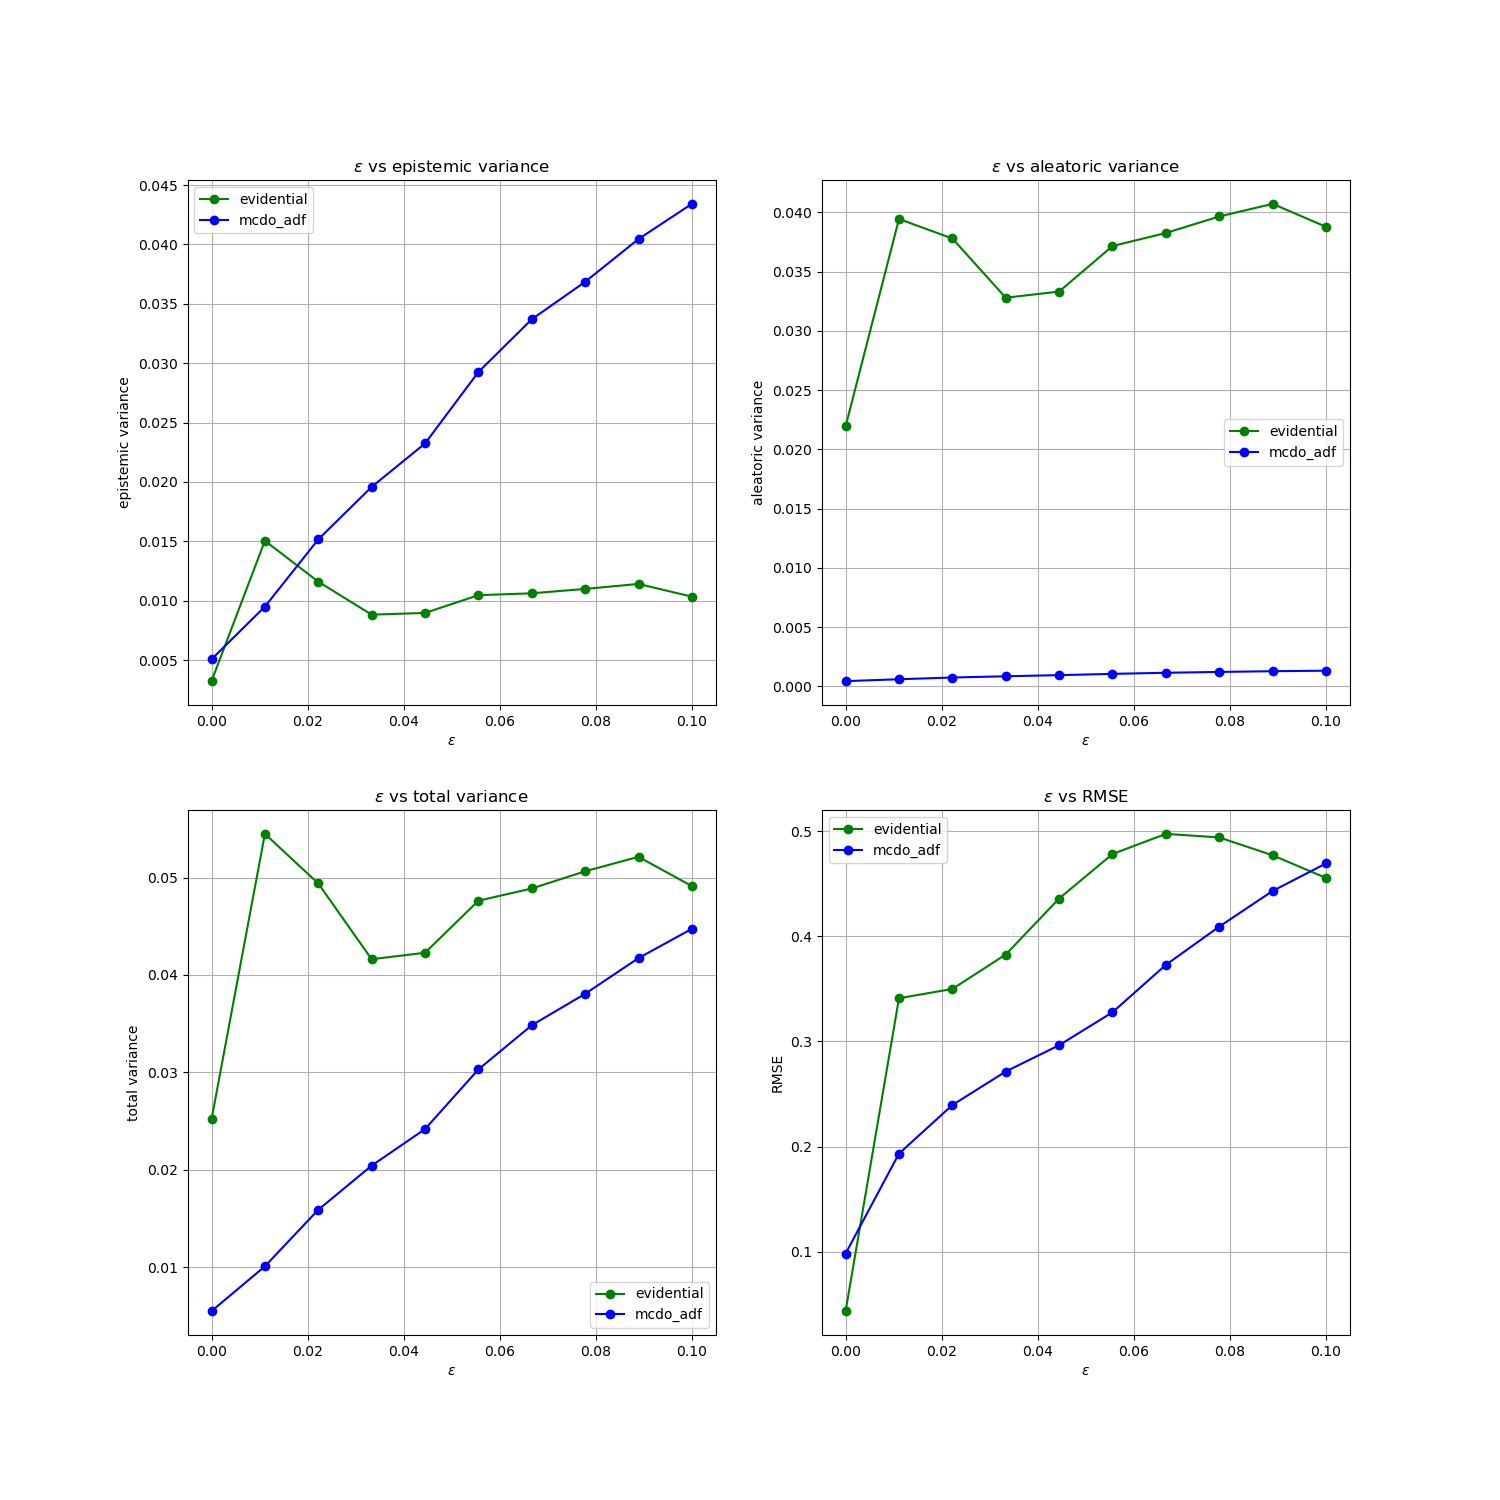
\includegraphics[scale=0.35]{adversarial/adv_plots}
	\caption{Plots of $\epsilon$(adversarial perturbations) against uncertainties and RMSE}
	\label{fig_adv_analysis}
\end{figure}
\subsubsection{Spearman's correlation analysis}

Spearman's rank correlation (often denoted by $\rho$) is a measure of statistical dependence between a pair of variables. Intuitively $\rho$ indicates the strength and direction of association between two ranked variables. $\rho$ varies between -1 and 1. The direction of association is indicated by sign of $\rho$ while its magnitude indicates the strength of correlation between the variable pair.

In the context of analyzing response of uncertainty estimation methods to adversarial attacks, Spearman's rank correlation coefficient is computed for pairs of following variables : $\epsilon$, absolute deviation of a prediction from its corresponding ground truth value, aleatoric, epistemic and total uncertainties. Though Pearson's correlation coefficient is a common choice for correlation analysis, there are two reasons to prefer Spearman's correlation for this analysis:
\begin{itemize}
	\item Pearson's correlation measure applies to normally distributed variables. As no assumptions are made on underlying distributions of the considered set of variables Spearman's correlation coefficient is preferred.
	\item Spearman's coefficient measures correlation between a pair of ranked variables. As this analysis focuses on effects of increasing levels of $\epsilon$ (a ranked variable) on other variables, the measure becomes an apt choice.
\end{itemize} 
Spearman's correlation coefficients are arranged in form of a symmetric matrix (indices denoting variables) separately for both MCDO\_ADF and DER model variants as shown in the figure below.
\begin{figure}[H]
	\begin{subfigure}[b]{0.55\textwidth}
		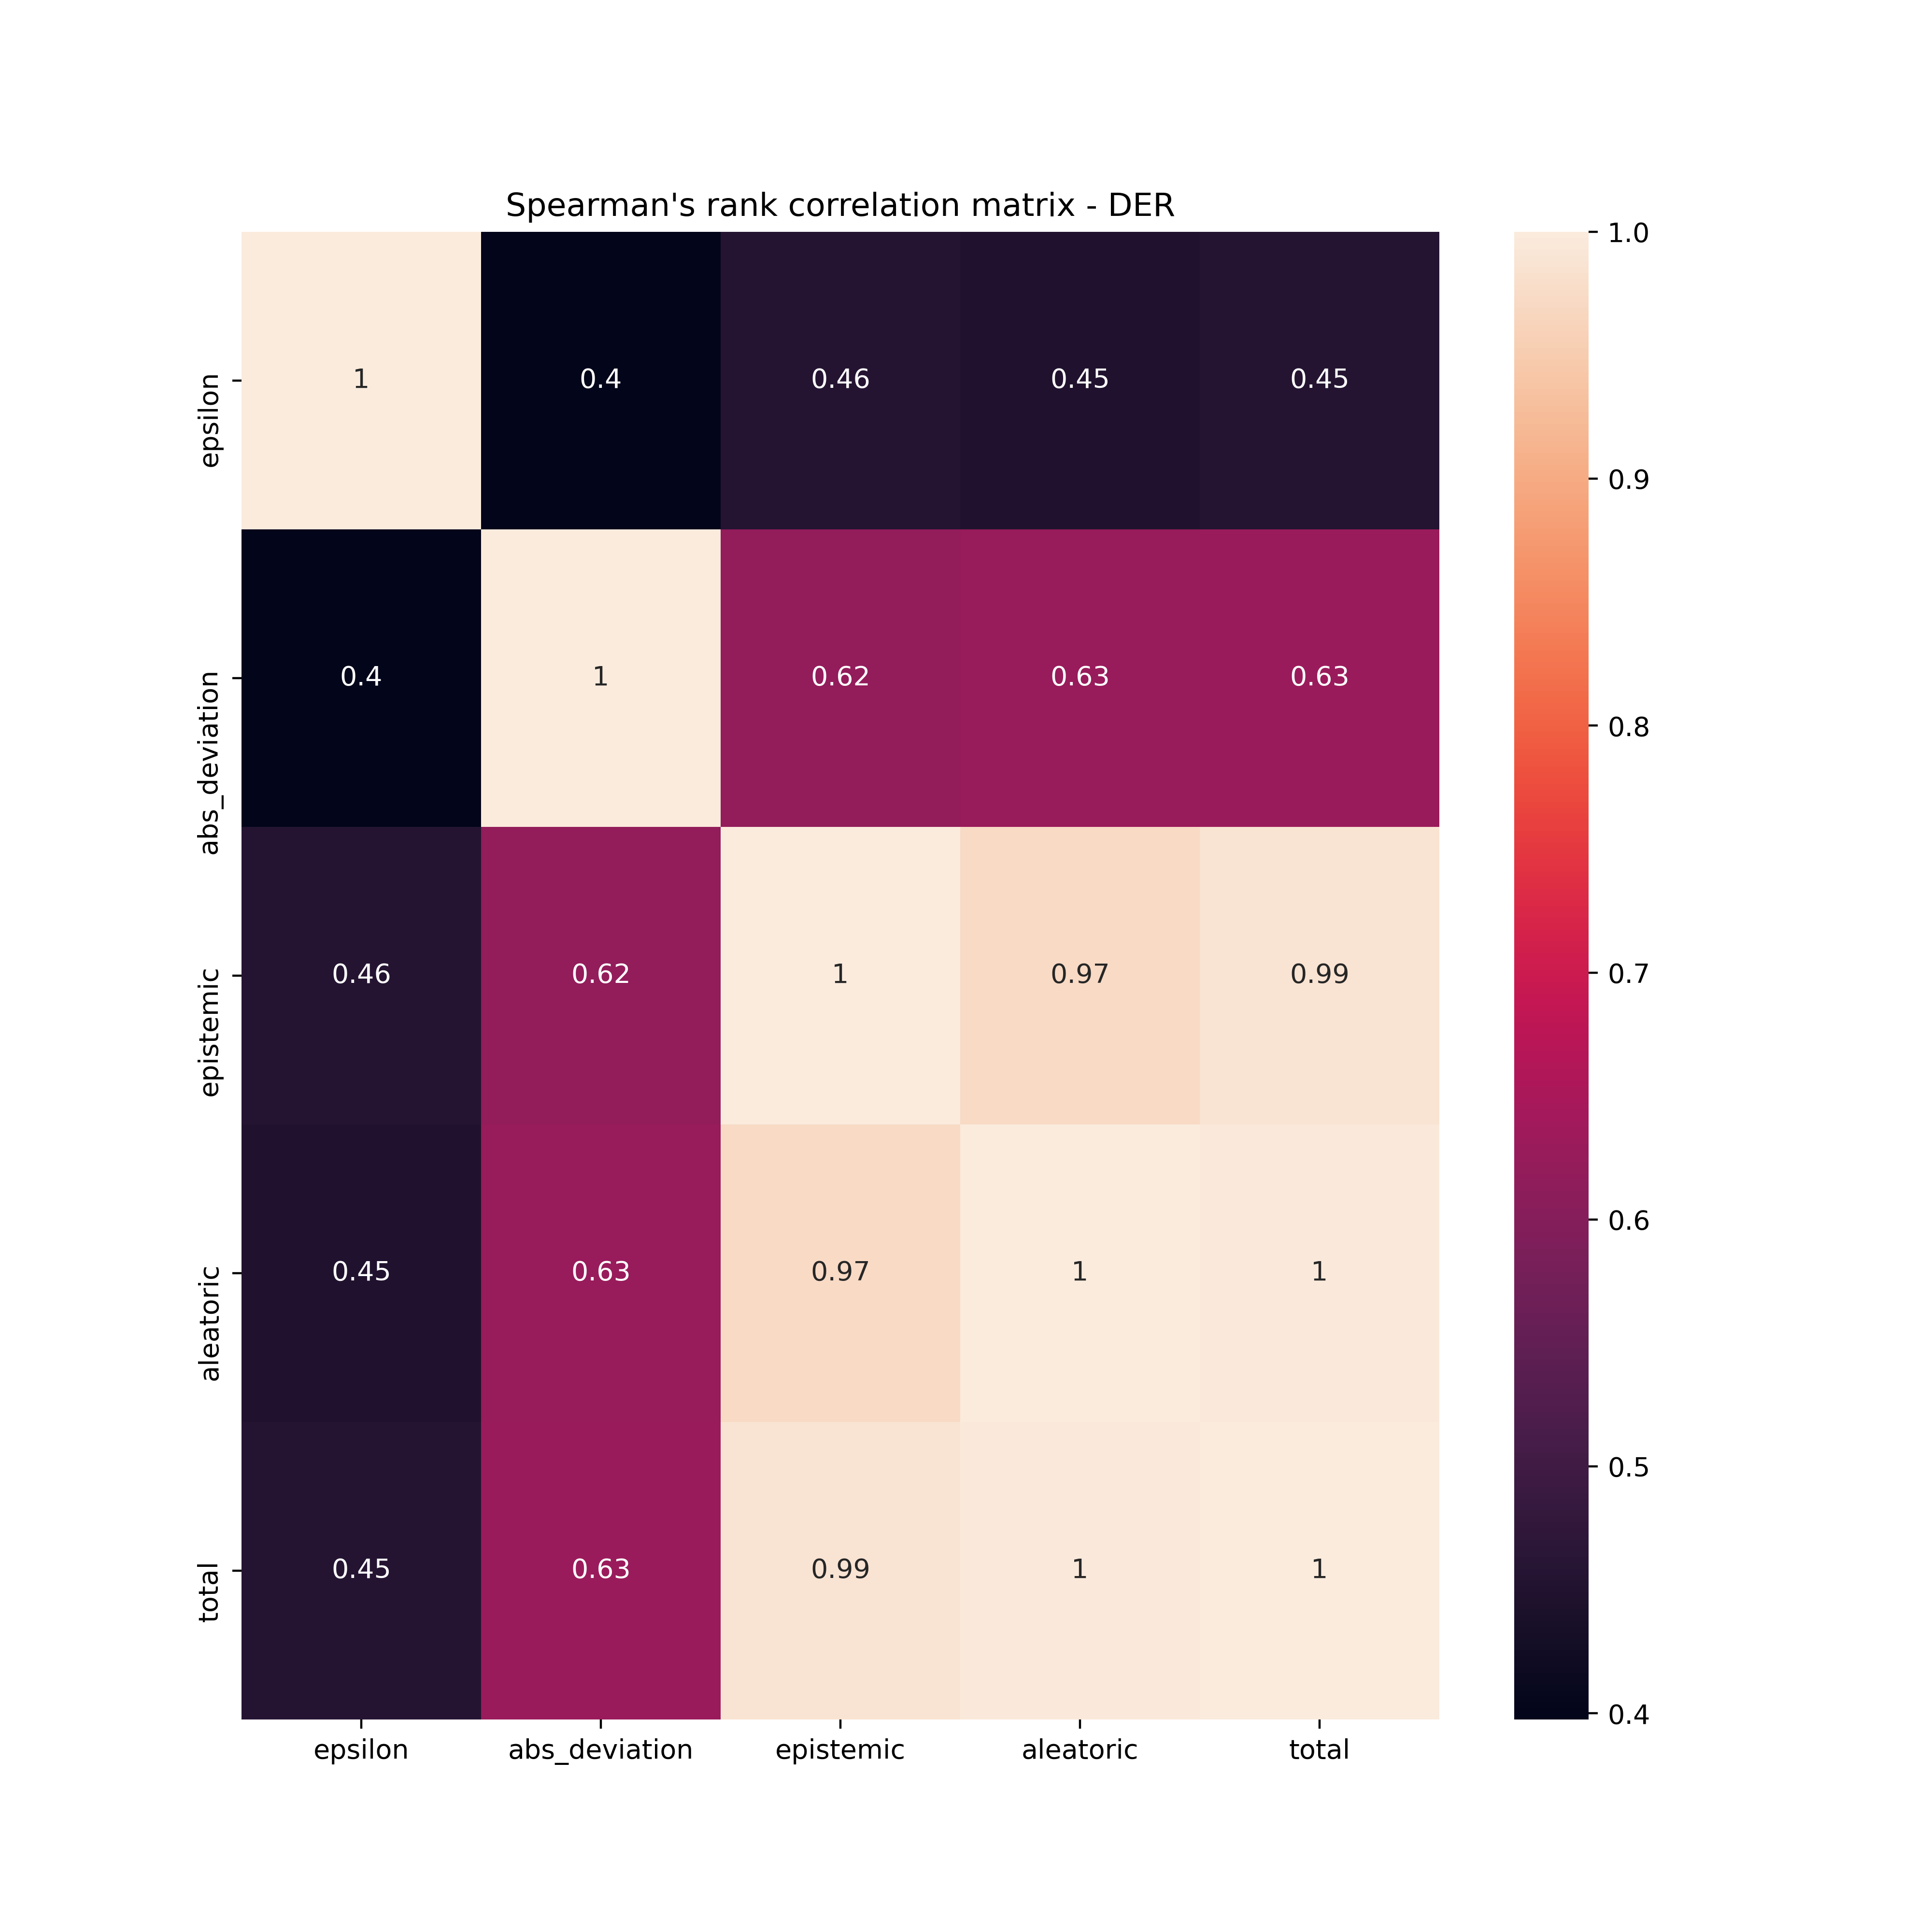
\includegraphics[width=\textwidth]{adversarial/evi_correlation_matrix}
		\caption{Spearman's correlation matrix for DER}
		\label{fig:five over x}
	\end{subfigure}
	\hfill
	\begin{subfigure}[b]{0.55\textwidth}
		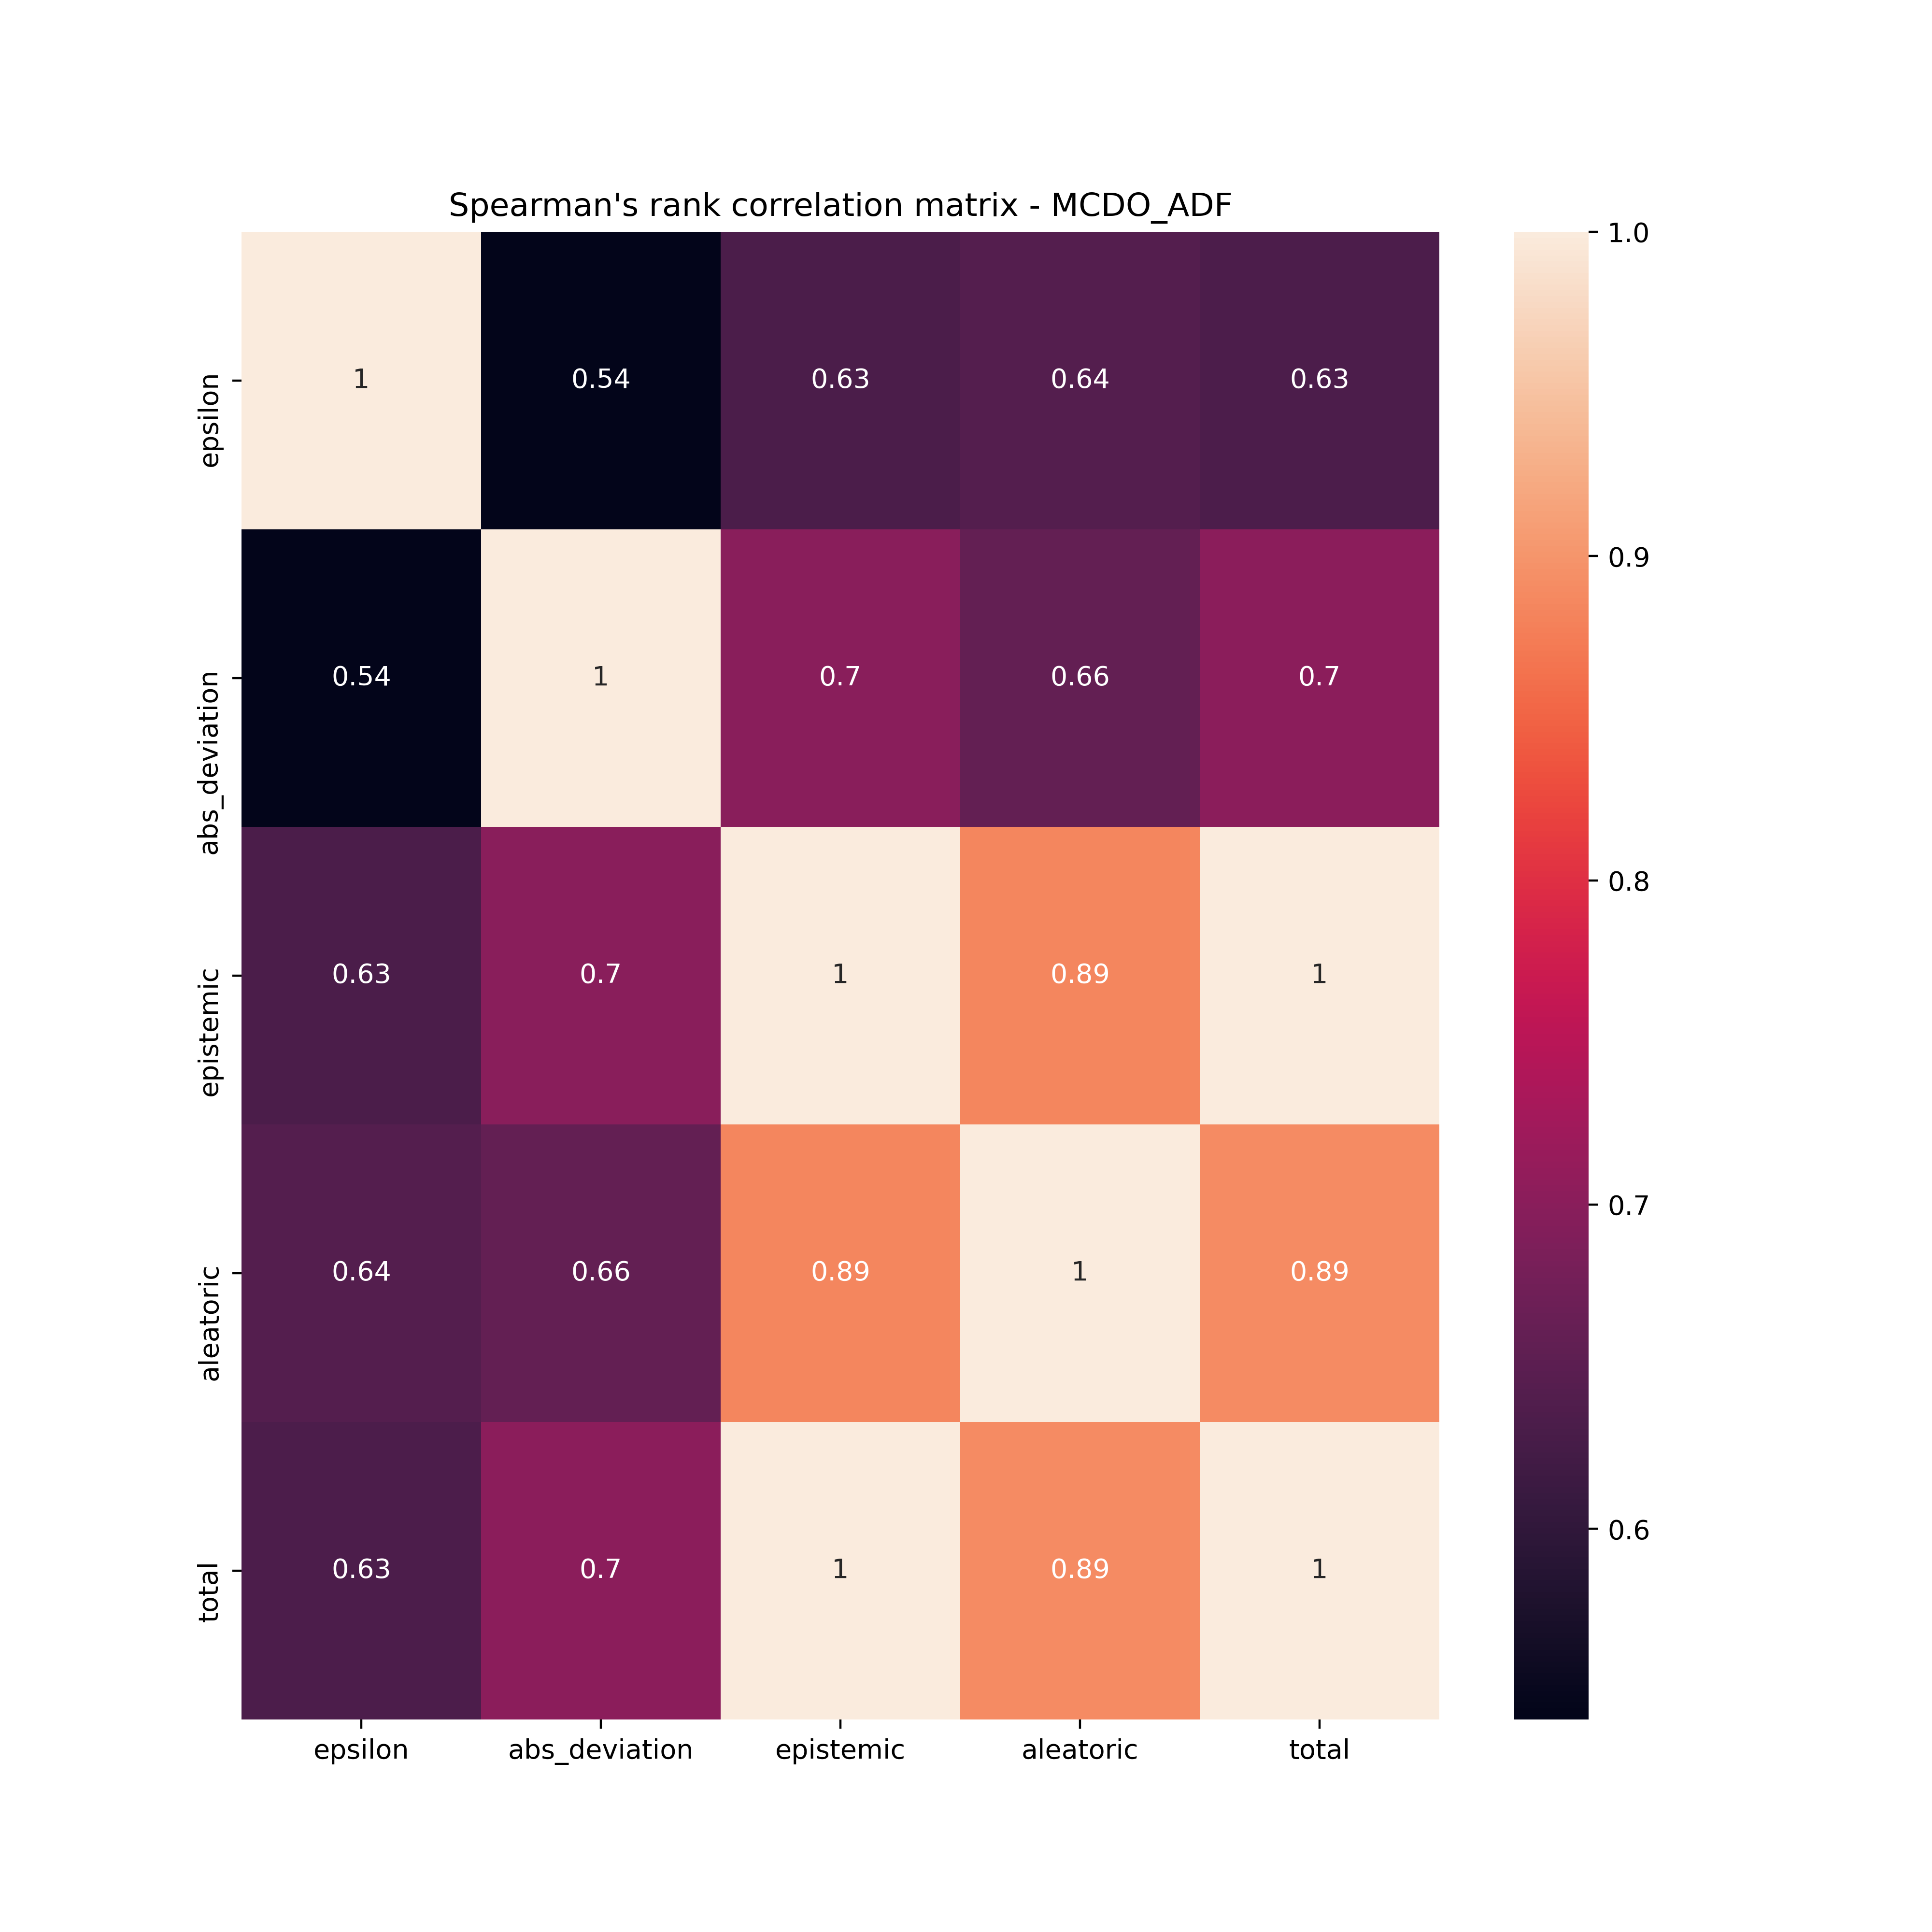
\includegraphics[width=\textwidth]{adversarial/mcdo_adf_correlation_matrix}
		\caption{Spearman's correlation matrix for MCDO\_ADF}
		\label{fig:five over x}
	\end{subfigure}
	\caption{Spearman's correlation heatmaps}
	\label{fig_correlation_analysis}
\end{figure}
The following can be inferred from the computed correlation coefficient matrices:
\begin{itemize}
	\item MCDO\_ADF shows relatively a stronger correlation between $\epsilon$ and other variables of interest than DER. This indicates a higher-level of alignment between $\epsilon$ and uncertainties estimated by MCDO\_ADF, which is desirable.
	\item A stronger association exists between epistemic and aleatoric components of uncertainty estimated by DER ($\rho = 0.97$) than MCDO\_ADF($\rho = 0.89$). This can be attributed to DER's ability to relate the pair of uncertainty components.
	\item The dominance of aleatoric and epistemic uncertainty components in total uncertainties estimated by DER and MCDO\_ADF respectively can observed in their corresponding correlation coefficients. This aligns with inferences obtained from \ref{fig_adv_analysis}. 
\end{itemize}

\section{Evaluation summary}

\begin{table}[H]
	\centering
	\begin{tabular}{|c|c|c|} 
		\hline
		\textbf{Experiment}                                                                                             & \textbf{Metric}                                                                                                            & \textbf{Better performer}   \\ 
		\hline
		\multirow{4}{*}{\begin{tabular}[c]{@{}c@{}}Udacity steering angle \\ test dataset evaluation \end{tabular}}     & NLL                                                                                                                        & DER                         \\ 
		\cline{2-3}
		& RMSE                                                                                                                       & DER                         \\ 
		\cline{2-3}
		& EVA                                                                                                                        & DER                         \\ 
		\cline{2-3}
		& Qualitative comparison                                                                                                     & MCDO\_ADF                   \\ 
		\hline
		\multirow{2}{*}{1D datasets}                                                                                    & NLL                                                                                                                        & DER                         \\ 
		\cline{2-3}
		& RMSE                                                                                                                       & MCDO\_ADF                   \\ 
		\hline
		\begin{tabular}[c]{@{}c@{}}Response to \\ adversarial attacks \end{tabular}                                     & \begin{tabular}[c]{@{}c@{}}Spearman's rank correlation\\ coefficient between \\perturbations and uncertainty \end{tabular} & MCDO\_ADF                   \\ 
		\hline
		\multirow{2}{*}{\begin{tabular}[c]{@{}c@{}}Response to Out-Of-Distribution inputs\\(1D datasets) \end{tabular}} & NLL                                                                                                                        & DER                         \\ 
		\cline{2-3}
		& RMSE                                                                                                                       & MCDO\_ADF                   \\
		\hline
	\end{tabular}
\caption{Table of conducted experiments and their results}
\label{tab_eval_summary}
\end{table}
The above table summarizes results from the set of experiments conducted in this research work. It can be inferred that there does not exist a single clear winner which outperforms the other in every conducted experiment. However, when it comes to evaluating the pair of methods based on uncertainty estimation quality, measured in terms of NLL, DER outperforms MCDO\_ADF in both the datasets considered. This signifies the higher likelihood of ground truth's presence in distributions outputted by DER integrated models, than its MCDO\_ADF counterparts. MCDO\_ADF performs better in terms of RMSE, a measure of predictive accuracy on both datasets. This can be attributed to the use of multiple MC samples by MCDO\_ADF models to output their predictions.When it comes to analyzing the pair of methods on Out-Of-Distribution inputs, MCDO\_ADF's response is desirable when inputs are adversarially perturbed, while DER's uncertainty estimates are more reliable when a model encounters inputs that lie outside the training data distribution. 

\end{document}
